\documentclass[twoside]{book}

% Packages required by doxygen
\usepackage{calc}
\usepackage{doxygen}
\usepackage{graphicx}
\usepackage[utf8]{inputenc}
\usepackage{makeidx}
\usepackage{multicol}
\usepackage{multirow}
\usepackage{textcomp}
\usepackage[table]{xcolor}

% Font selection
\usepackage[T1]{fontenc}
\usepackage{mathptmx}
\usepackage[scaled=.90]{helvet}
\usepackage{courier}
\usepackage{amssymb}
\usepackage{sectsty}
\renewcommand{\familydefault}{\sfdefault}
\allsectionsfont{%
  \fontseries{bc}\selectfont%
  \color{darkgray}%
}
\renewcommand{\DoxyLabelFont}{%
  \fontseries{bc}\selectfont%
  \color{darkgray}%
}

% Page & text layout
\usepackage{geometry}
\geometry{%
  a4paper,%
  top=2.5cm,%
  bottom=2.5cm,%
  left=2.5cm,%
  right=2.5cm%
}
\tolerance=750
\hfuzz=15pt
\hbadness=750
\setlength{\emergencystretch}{15pt}
\setlength{\parindent}{0cm}
\setlength{\parskip}{0.2cm}
\makeatletter
\renewcommand{\paragraph}{%
  \@startsection{paragraph}{4}{0ex}{-1.0ex}{1.0ex}{%
    \normalfont\normalsize\bfseries\SS@parafont%
  }%
}
\renewcommand{\subparagraph}{%
  \@startsection{subparagraph}{5}{0ex}{-1.0ex}{1.0ex}{%
    \normalfont\normalsize\bfseries\SS@subparafont%
  }%
}
\makeatother

% Headers & footers
\usepackage{fancyhdr}
\pagestyle{fancyplain}
\fancyhead[LE]{\fancyplain{}{\bfseries\thepage}}
\fancyhead[CE]{\fancyplain{}{}}
\fancyhead[RE]{\fancyplain{}{\bfseries\leftmark}}
\fancyhead[LO]{\fancyplain{}{\bfseries\rightmark}}
\fancyhead[CO]{\fancyplain{}{}}
\fancyhead[RO]{\fancyplain{}{\bfseries\thepage}}
\fancyfoot[LE]{\fancyplain{}{}}
\fancyfoot[CE]{\fancyplain{}{}}
\fancyfoot[RE]{\fancyplain{}{\bfseries\scriptsize Generated on Mon Sep 2 2013 22:28:57 for Crowbar by Doxygen }}
\fancyfoot[LO]{\fancyplain{}{\bfseries\scriptsize Generated on Mon Sep 2 2013 22:28:57 for Crowbar by Doxygen }}
\fancyfoot[CO]{\fancyplain{}{}}
\fancyfoot[RO]{\fancyplain{}{}}
\renewcommand{\footrulewidth}{0.4pt}
\renewcommand{\chaptermark}[1]{%
  \markboth{#1}{}%
}
\renewcommand{\sectionmark}[1]{%
  \markright{\thesection\ #1}%
}

% Indices & bibliography
\usepackage{natbib}
\usepackage[titles]{tocloft}
\setcounter{tocdepth}{3}
\setcounter{secnumdepth}{5}
\makeindex

% Hyperlinks (required, but should be loaded last)
\usepackage{ifpdf}
\ifpdf
  \usepackage[pdftex,pagebackref=true]{hyperref}
\else
  \usepackage[ps2pdf,pagebackref=true]{hyperref}
\fi
\hypersetup{%
  colorlinks=true,%
  linkcolor=blue,%
  citecolor=blue,%
  unicode%
}

% Custom commands
\newcommand{\clearemptydoublepage}{%
  \newpage{\pagestyle{empty}\cleardoublepage}%
}


%===== C O N T E N T S =====

\begin{document}

% Titlepage & ToC
\hypersetup{pageanchor=false}
\pagenumbering{roman}
\begin{titlepage}
\vspace*{7cm}
\begin{center}%
{\Large Crowbar \\[1ex]\large 1a9bd335b9 }\\
\vspace*{1cm}
{\large Generated by Doxygen 1.8.4}\\
\vspace*{0.5cm}
{\small Mon Sep 2 2013 22:28:57}\\
\end{center}
\end{titlepage}
\clearemptydoublepage
\tableofcontents
\clearemptydoublepage
\pagenumbering{arabic}
\hypersetup{pageanchor=true}

%--- Begin generated contents ---
\chapter{Crowbar}
\label{md_README}
\hypertarget{md_README}{}
An open-\/source level editor for Source games, built using Qt5.

Crowbar is built to improve on what Valve's Hammer, largely unchanged since the days of Quake, lacks in terms of functionality and ease of use. Built using the Qt5 framework, Crowbar is compatible with Windows, Mac and Linux and is created from the ground up to be modular and easily extensible. It supports scripting for basic tasks as well as the creation of custom C++ plugins for more advanced or performance-\/critical functions. 
\chapter{Module Index}
\section{Modules}
Here is a list of all modules\-:\begin{DoxyCompactList}
\item \contentsline{section}{Global variables}{\pageref{group___global_variables}}{}
\item \contentsline{section}{I\-Console library}{\pageref{group___i_console}}{}
\end{DoxyCompactList}

\chapter{Hierarchical Index}
\section{Class Hierarchy}
This inheritance list is sorted roughly, but not completely, alphabetically\-:\begin{DoxyCompactList}
\item \contentsline{section}{Geom\-Info}{\pageref{struct_geom_info}}{}
\item \contentsline{section}{Geom\-Meta\-Handle}{\pageref{class_geom_meta_handle}}{}
\begin{DoxyCompactList}
\item \contentsline{section}{Edge3\-D}{\pageref{class_edge3_d}}{}
\item \contentsline{section}{Face3\-D}{\pageref{class_face3_d}}{}
\item \contentsline{section}{Solid3\-D}{\pageref{class_solid3_d}}{}
\item \contentsline{section}{Vertex3\-D}{\pageref{class_vertex3_d}}{}
\end{DoxyCompactList}
\item \contentsline{section}{I\-Command\-Box}{\pageref{class_i_command_box}}{}
\item \contentsline{section}{I\-Command\-Manager}{\pageref{class_i_command_manager}}{}
\item \contentsline{section}{I\-Completion\-Widget}{\pageref{class_i_completion_widget}}{}
\item \contentsline{section}{I\-Console\-Window}{\pageref{class_i_console_window}}{}
\begin{DoxyCompactList}
\item \contentsline{section}{Console\-Window}{\pageref{class_console_window}}{}
\end{DoxyCompactList}
\item \contentsline{section}{I\-Plugin}{\pageref{class_i_plugin}}{}
\item \contentsline{section}{I\-Vertex3\-D\-Render\-Spec}{\pageref{class_i_vertex3_d_render_spec}}{}
\begin{DoxyCompactList}
\item \contentsline{section}{Vertex3\-D}{\pageref{class_vertex3_d}}{}
\end{DoxyCompactList}
\item \contentsline{section}{Plane}{\pageref{class_plane}}{}
\item Q\-List\-Widget\begin{DoxyCompactList}
\item \contentsline{section}{Completion\-List}{\pageref{class_completion_list}}{}
\end{DoxyCompactList}
\item Q\-Main\-Window\begin{DoxyCompactList}
\item \contentsline{section}{Main\-Win}{\pageref{class_main_win}}{}
\end{DoxyCompactList}
\item Q\-Object\begin{DoxyCompactList}
\item \contentsline{section}{Command\-Line\-Parser}{\pageref{class_command_line_parser}}{}
\item \contentsline{section}{Index\-Pool}{\pageref{class_index_pool}}{}
\item \contentsline{section}{Map\-Doc}{\pageref{class_map_doc}}{}
\item \contentsline{section}{Plugin\-Manager}{\pageref{class_plugin_manager}}{}
\end{DoxyCompactList}
\item Q\-Text\-Edit\begin{DoxyCompactList}
\item \contentsline{section}{Console\-Window}{\pageref{class_console_window}}{}
\end{DoxyCompactList}
\item Q\-Widget\begin{DoxyCompactList}
\item \contentsline{section}{Log\-Window}{\pageref{class_log_window}}{}
\end{DoxyCompactList}
\end{DoxyCompactList}

\chapter{Class Index}
\section{Class List}
Here are the classes, structs, unions and interfaces with brief descriptions\-:\begin{DoxyCompactList}
\item\contentsline{section}{\hyperlink{class_command_line_parser}{Command\-Line\-Parser} \\*Deals with arguments passed to the application on the command-\/line }{\pageref{class_command_line_parser}}{}
\item\contentsline{section}{\hyperlink{class_completion_list}{Completion\-List} }{\pageref{class_completion_list}}{}
\item\contentsline{section}{\hyperlink{class_console_window}{Console\-Window} }{\pageref{class_console_window}}{}
\item\contentsline{section}{\hyperlink{class_edge3_d}{Edge3\-D} \\*An edge links two vertices and two faces, referenced by their geometry handles.\par
 When considering travelling along the edge from the beginning to end vertex, the normals of the faces either side of the edge can be considered to point clockwise or anticlockwise around the edge. The face with an anticlockwise-\/pointing normal is denoted the \char`\"{}right\char`\"{} face (if the normal were pointing upwards the face would be positioned to the right of the edge) and the face with the clockwise-\/pointing normal is denoted the \char`\"{}left\char`\"{} face. If both normals are pointing in the same direction (either clockwise or anticlockwise) it is not defined which face is denoted left and which right }{\pageref{class_edge3_d}}{}
\item\contentsline{section}{\hyperlink{class_face3_d}{Face3\-D} \\*Class representing a 3\-D face }{\pageref{class_face3_d}}{}
\item\contentsline{section}{\hyperlink{struct_geom_info}{Geom\-Info} \\*Struct to hold and pass information about geometry objects }{\pageref{struct_geom_info}}{}
\item\contentsline{section}{\hyperlink{class_geom_meta_handle}{Geom\-Meta\-Handle} \\*Metaclass which all geometry components subclass from. Contains useful metadata relevant to geometry components }{\pageref{class_geom_meta_handle}}{}
\item\contentsline{section}{\hyperlink{class_i_command_box}{I\-Command\-Box} }{\pageref{class_i_command_box}}{}
\item\contentsline{section}{\hyperlink{class_i_command_manager}{I\-Command\-Manager} }{\pageref{class_i_command_manager}}{}
\item\contentsline{section}{\hyperlink{class_i_completion_widget}{I\-Completion\-Widget} }{\pageref{class_i_completion_widget}}{}
\item\contentsline{section}{\hyperlink{class_i_console_window}{I\-Console\-Window} }{\pageref{class_i_console_window}}{}
\item\contentsline{section}{\hyperlink{class_index_pool}{Index\-Pool} \\*Manages non-\/consecutive array indices }{\pageref{class_index_pool}}{}
\item\contentsline{section}{\hyperlink{class_i_plugin}{I\-Plugin} \\*Required core interface for a Crowbar plugin }{\pageref{class_i_plugin}}{}
\item\contentsline{section}{\hyperlink{class_i_vertex3_d_render_spec}{I\-Vertex3\-D\-Render\-Spec} \\*Defines the properties required to be exposed by renderable vertices }{\pageref{class_i_vertex3_d_render_spec}}{}
\item\contentsline{section}{\hyperlink{class_log_window}{Log\-Window} \\*Logging window }{\pageref{class_log_window}}{}
\item\contentsline{section}{\hyperlink{class_main_win}{Main\-Win} \\*Application window class }{\pageref{class_main_win}}{}
\item\contentsline{section}{\hyperlink{class_map_doc}{Map\-Doc} \\*The \hyperlink{class_map_doc}{Map\-Doc} class }{\pageref{class_map_doc}}{}
\item\contentsline{section}{\hyperlink{class_plane}{Plane} \\*Defines a plane in 3\-D space }{\pageref{class_plane}}{}
\item\contentsline{section}{\hyperlink{class_plugin_manager}{Plugin\-Manager} \\*Manages loading of plugins }{\pageref{class_plugin_manager}}{}
\item\contentsline{section}{\hyperlink{class_solid3_d}{Solid3\-D} \\*Class representing a 3\-D solid }{\pageref{class_solid3_d}}{}
\item\contentsline{section}{\hyperlink{class_vertex3_d}{Vertex3\-D} \\*Defines a vertex in 3\-D space }{\pageref{class_vertex3_d}}{}
\end{DoxyCompactList}

\chapter{File Index}
\section{File List}
Here is a list of all documented files with brief descriptions\-:\begin{DoxyCompactList}
\item\contentsline{section}{app/\hyperlink{commandlineparser_8h}{commandlineparser.\-h} \\*Defines the class responsible for parsing command-\/line arguments and setting the relevant settings in response }{\pageref{commandlineparser_8h}}{}
\item\contentsline{section}{app/{\bfseries consolewindow.\-h} }{\pageref{consolewindow_8h}}{}
\item\contentsline{section}{app/\hyperlink{edge_8h}{edge.\-h} \\*Defines an edge which links two vertices }{\pageref{edge_8h}}{}
\item\contentsline{section}{app/\hyperlink{face_8h}{face.\-h} \\*Defines a 3\-D face. Solids are built up of these faces. Faces reference edges, which in turn reference vertices }{\pageref{face_8h}}{}
\item\contentsline{section}{app/\hyperlink{globals_8h}{globals.\-h} \\*Defines global variables and classes }{\pageref{globals_8h}}{}
\item\contentsline{section}{app/\hyperlink{indexpool_8h}{indexpool.\-h} \\*Defines the \hyperlink{class_index_pool}{Index\-Pool} class which manages non-\/consecutive array indices }{\pageref{indexpool_8h}}{}
\item\contentsline{section}{app/\hyperlink{ivertex3drenderspec_8h}{ivertex3drenderspec.\-h} \\*Defines the interface between map vertices and the vertices used for rendering }{\pageref{ivertex3drenderspec_8h}}{}
\item\contentsline{section}{app/\hyperlink{mainwin_8h}{mainwin.\-h} \\*Defines a main application window corresponding to one currently open map document }{\pageref{mainwin_8h}}{}
\item\contentsline{section}{app/\hyperlink{mapdoc_8h}{mapdoc.\-h} \\*The main map document class }{\pageref{mapdoc_8h}}{}
\item\contentsline{section}{app/\hyperlink{matlib_8h}{matlib.\-h} \\*Contains convenient custom maths functions }{\pageref{matlib_8h}}{}
\item\contentsline{section}{app/{\bfseries openglwidget.\-h} }{\pageref{openglwidget_8h}}{}
\item\contentsline{section}{app/\hyperlink{plane_8h}{plane.\-h} \\*Defines a plane class to hold the co-\/ordinates of a plane in 3\-D space }{\pageref{plane_8h}}{}
\item\contentsline{section}{app/\hyperlink{solid_8h}{solid.\-h} \\*Defines a solid class }{\pageref{solid_8h}}{}
\item\contentsline{section}{app/\hyperlink{vertex_8h}{vertex.\-h} \\*T\-O\-D\-O }{\pageref{vertex_8h}}{}
\item\contentsline{section}{I\-Console/inc/\hyperlink{baseconsolecommand_8h}{baseconsolecommand.\-h} \\*Describes the base properties common to all console commands and variables }{\pageref{baseconsolecommand_8h}}{}
\item\contentsline{section}{I\-Console/inc/\hyperlink{commandentrybox_8h}{commandentrybox.\-h} \\*Defines the \hyperlink{class_command_entry_box}{Command\-Entry\-Box} class which manages the input of console commands by the user }{\pageref{commandentrybox_8h}}{}
\item\contentsline{section}{I\-Console/inc/\hyperlink{commandinterpreter_8h}{commandinterpreter.\-h} \\*Defines the \hyperlink{class_command_interpreter}{Command\-Interpreter} class to interpret raw user-\/input command strings }{\pageref{commandinterpreter_8h}}{}
\item\contentsline{section}{I\-Console/inc/\hyperlink{commandmanager_8h}{commandmanager.\-h} \\*Defines the \hyperlink{class_command_manager}{Command\-Manager} class which allows quick searching for a console command or variable by name }{\pageref{commandmanager_8h}}{}
\item\contentsline{section}{I\-Console/inc/\hyperlink{commandsenderinfo_8h}{commandsenderinfo.\-h} }{\pageref{commandsenderinfo_8h}}{}
\item\contentsline{section}{I\-Console/inc/{\bfseries commandsuggestionlist.\-h} }{\pageref{commandsuggestionlist_8h}}{}
\item\contentsline{section}{I\-Console/inc/{\bfseries concommand.\-h} }{\pageref{concommand_8h}}{}
\item\contentsline{section}{I\-Console/inc/{\bfseries consolewidget.\-h} }{\pageref{consolewidget_8h}}{}
\item\contentsline{section}{I\-Console/inc/{\bfseries convar.\-h} }{\pageref{convar_8h}}{}
\item\contentsline{section}{I\-Console/inc/\hyperlink{iconsole__global_8h}{iconsole\-\_\-global.\-h} \\*Defines some global properties for the library }{\pageref{iconsole__global_8h}}{}
\item\contentsline{section}{I\-Console/inc/{\bfseries listedcommandmanager.\-h} }{\pageref{listedcommandmanager_8h}}{}
\item\contentsline{section}{I\-Console/inc/{\bfseries listedconsolecommand.\-h} }{\pageref{listedconsolecommand_8h}}{}
\item\contentsline{section}{I\-Console/inc/\hyperlink{nglobalcmd_8h}{nglobalcmd.\-h} \\*Defines global properties for console commands }{\pageref{nglobalcmd_8h}}{}
\item\contentsline{section}{I\-Console/inc/{\bfseries wr\-\_\-commandentrybox.\-h} }{\pageref{wr__commandentrybox_8h}}{}
\item\contentsline{section}{I\-Console/inc/{\bfseries wr\-\_\-commandinterpreter.\-h} }{\pageref{wr__commandinterpreter_8h}}{}
\item\contentsline{section}{I\-Console/inc/{\bfseries wr\-\_\-commandmanager.\-h} }{\pageref{wr__commandmanager_8h}}{}
\item\contentsline{section}{I\-Console/inc/{\bfseries wr\-\_\-concommand.\-h} }{\pageref{wr__concommand_8h}}{}
\item\contentsline{section}{I\-Console/inc/{\bfseries wr\-\_\-convar.\-h} }{\pageref{wr__convar_8h}}{}
\item\contentsline{section}{I\-Console/inc/{\bfseries wr\-\_\-listedcommandmanager.\-h} }{\pageref{wr__listedcommandmanager_8h}}{}
\item\contentsline{section}{I\-Console/inc/{\bfseries wr\-\_\-listedconsolecommand.\-h} }{\pageref{wr__listedconsolecommand_8h}}{}
\end{DoxyCompactList}

\chapter{Module Documentation}
\hypertarget{group___global_variables}{\section{Global variables}
\label{group___global_variables}\index{Global variables@{Global variables}}
}
\subsection*{Macros}
\begin{DoxyCompactItemize}
\item 
\hypertarget{group___global_variables_gaf9c6d8de2e7b3d11f070bb500d62edce}{\#define {\bfseries D\-E\-F\-I\-N\-E\-\_\-\-C\-O\-N\-V\-A\-R}(sz\-Name\-\_\-\-No\-Quote, sz\-Def\-Val, p\-Callback, sz\-Desc, i\-Flags, b\-Min, fl\-Min, b\-Max, fl\-Max)~\hyperlink{class_con_var}{Con\-Var} sz\-Name\-\_\-\-No\-Quote(\#sz\-Name\-\_\-\-No\-Quote, sz\-Def\-Val, \hyperlink{group___global_variables_ga4d39defaa5d22f29bde4c75d590bd0fe}{g\-\_\-p\-Command\-Manager}, \&\hyperlink{group___global_variables_ga8389c826239a1bc627ae3b7f97a79fe4}{g\-\_\-p\-Command\-List}, p\-Callback, sz\-Desc, i\-Flags, b\-Min, fl\-Min, b\-Max, fl\-Max);}\label{group___global_variables_gaf9c6d8de2e7b3d11f070bb500d62edce}

\item 
\hypertarget{group___global_variables_ga5c65583f94cc62a481b1846c0e6e3344}{\#define {\bfseries D\-E\-F\-I\-N\-E\-\_\-\-C\-O\-N\-C\-O\-M\-M\-A\-N\-D}(sz\-Name\-\_\-\-No\-Quote, p\-Callback, sz\-Desc, i\-Flags)~\hyperlink{class_con_command}{Con\-Command} sz\-Name\-\_\-\-No\-Quote(\#sz\-Name\-\_\-\-No\-Quote, p\-Callback, \hyperlink{group___global_variables_ga4d39defaa5d22f29bde4c75d590bd0fe}{g\-\_\-p\-Command\-Manager}, \&\hyperlink{group___global_variables_ga8389c826239a1bc627ae3b7f97a79fe4}{g\-\_\-p\-Command\-List}, sz\-Desc, i\-Flags);}\label{group___global_variables_ga5c65583f94cc62a481b1846c0e6e3344}

\end{DoxyCompactItemize}
\subsection*{Functions}
\begin{DoxyCompactItemize}
\item 
void \hyperlink{group___global_variables_ga9551f73a6927861d0b6f5d7901c90888}{Show\-Message\-Box} (Q\-String message)
\begin{DoxyCompactList}\small\item\em Creates a basic one-\/time modal message box with simple message and an \char`\"{}\-O\-K\char`\"{} button. \end{DoxyCompactList}\item 
void \hyperlink{group___global_variables_gadf8a13f3d23660f424828d7f559addd3}{Show\-Error\-Box} (Q\-String message)
\begin{DoxyCompactList}\small\item\em Creates a basic one-\/time modal error box with simple message and an \char`\"{}\-O\-K\char`\"{} button. \end{DoxyCompactList}\item 
void \hyperlink{group___global_variables_ga1788dc69b89b298a038015cbb83f8183}{Log\-Message} (const Q\-String \&message, bool newline=true)
\begin{DoxyCompactList}\small\item\em Logs a message to the log window. \end{DoxyCompactList}\item 
void \hyperlink{group___global_variables_gacb9fa8876388ad9319c61d9ae4d21510}{Log\-Tagged\-Message} (const Q\-String \&tag, const Q\-String \&message, bool newline=true)
\begin{DoxyCompactList}\small\item\em Logs a tagged message. \end{DoxyCompactList}\item 
void \hyperlink{group___global_variables_ga4b2863ab23932e06f2b5f292c66e7ef6}{Log\-Warning} (const Q\-String \&message, bool newline=true)
\begin{DoxyCompactList}\small\item\em Logs a warning to the log window. Log text is printed red and in bold. \end{DoxyCompactList}\item 
void \hyperlink{group___global_variables_ga49e471be032d9340fe6b4c251d1aef21}{Log\-Tagged\-Warning} (const Q\-String \&tag, const Q\-String \&message, bool newline=true)
\begin{DoxyCompactList}\small\item\em Logs a tagged warning to the log window. Log text is printed red and in bold. \end{DoxyCompactList}\item 
\hypertarget{group___global_variables_gab9e5c16962c3cdcd7220de6dfa5a70b5}{void {\bfseries Log\-Output} (\hyperlink{class_command_sender_info_a3a5e6a2ef1772f6557f351652c2e3b60}{Command\-Sender\-Info\-::\-Output\-Type} type, const Q\-String \&message, bool newline=true)}\label{group___global_variables_gab9e5c16962c3cdcd7220de6dfa5a70b5}

\item 
\hypertarget{group___global_variables_ga63348a368c397865f05d9a17c94752c6}{void {\bfseries Log\-Tagged\-Output} (\hyperlink{class_command_sender_info_a3a5e6a2ef1772f6557f351652c2e3b60}{Command\-Sender\-Info\-::\-Output\-Type} type, const Q\-String \&tag, const Q\-String \&message, bool newline=true)}\label{group___global_variables_ga63348a368c397865f05d9a17c94752c6}

\end{DoxyCompactItemize}
\subsection*{Variables}
\begin{DoxyCompactItemize}
\item 
\hyperlink{class_command_line_parser}{Command\-Line\-Parser} $\ast$ \hyperlink{group___global_variables_ga270fc6d9322b018e011978d6376f43ba}{g\-\_\-p\-Cmd\-Line}
\begin{DoxyCompactList}\small\item\em Global command-\/line parser object. \end{DoxyCompactList}\item 
\hyperlink{class_console_window}{Console\-Window} $\ast$ \hyperlink{group___global_variables_gae2d76408535137add345d6e4258c5a07}{g\-\_\-p\-Log}
\begin{DoxyCompactList}\small\item\em Global console window object. \end{DoxyCompactList}\item 
Q\-List$<$ \hyperlink{class_main_win}{Main\-Win} $\ast$ $>$ $\ast$ \hyperlink{group___global_variables_gab5d481b5087f9956e533067ad8001d78}{g\-\_\-p\-Window\-Tracker}
\begin{DoxyCompactList}\small\item\em Global window tracker object. \end{DoxyCompactList}\item 
\hyperlink{class_listed_command_manager}{Listed\-Command\-Manager} $\ast$ \hyperlink{group___global_variables_ga4d39defaa5d22f29bde4c75d590bd0fe}{g\-\_\-p\-Command\-Manager}
\begin{DoxyCompactList}\small\item\em Global console command manager, created in main.\-cpp. \end{DoxyCompactList}\item 
\hypertarget{group___global_variables_ga347a4723fad5c3711958f787dfc93fa4}{\hyperlink{class_command_interpreter}{Command\-Interpreter} $\ast$ \hyperlink{group___global_variables_ga347a4723fad5c3711958f787dfc93fa4}{g\-\_\-p\-Command\-Interpreter}}\label{group___global_variables_ga347a4723fad5c3711958f787dfc93fa4}

\begin{DoxyCompactList}\small\item\em Global console command interpreter, created in main.\-cpp. \end{DoxyCompactList}\item 
\hyperlink{class_listed_console_command}{Listed\-Console\-Command} $\ast$ \hyperlink{group___global_variables_ga8389c826239a1bc627ae3b7f97a79fe4}{g\-\_\-p\-Command\-List}
\begin{DoxyCompactList}\small\item\em Global console command list pointer. \end{DoxyCompactList}\end{DoxyCompactItemize}


\subsection{Detailed Description}


\subsection{Function Documentation}
\hypertarget{group___global_variables_ga1788dc69b89b298a038015cbb83f8183}{\index{Global variables@{Global variables}!Log\-Message@{Log\-Message}}
\index{Log\-Message@{Log\-Message}!Global variables@{Global variables}}
\subsubsection[{Log\-Message}]{\setlength{\rightskip}{0pt plus 5cm}void Log\-Message (
\begin{DoxyParamCaption}
\item[{const Q\-String \&}]{message, }
\item[{bool}]{newline = {\ttfamily true}}
\end{DoxyParamCaption}
)}}\label{group___global_variables_ga1788dc69b89b298a038015cbb83f8183}


Logs a message to the log window. 

Messages can be formatted by passing Q\-String(\char`\"{}\%0 \%1 ...\char`\"{}).arg(arg0).arg(arg1)... as the message parameter. 
\begin{DoxyParams}{Parameters}
{\em message} & Message to write. \\
\hline
{\em newline} & Whether a newline should follow the message. Defaults to true. \\
\hline
\end{DoxyParams}
\hypertarget{group___global_variables_gacb9fa8876388ad9319c61d9ae4d21510}{\index{Global variables@{Global variables}!Log\-Tagged\-Message@{Log\-Tagged\-Message}}
\index{Log\-Tagged\-Message@{Log\-Tagged\-Message}!Global variables@{Global variables}}
\subsubsection[{Log\-Tagged\-Message}]{\setlength{\rightskip}{0pt plus 5cm}void Log\-Tagged\-Message (
\begin{DoxyParamCaption}
\item[{const Q\-String \&}]{tag, }
\item[{const Q\-String \&}]{message, }
\item[{bool}]{newline = {\ttfamily true}}
\end{DoxyParamCaption}
)}}\label{group___global_variables_gacb9fa8876388ad9319c61d9ae4d21510}


Logs a tagged message. 

Messages can be formatted by passing Q\-String(\char`\"{}\%0 \%1 ...\char`\"{}).arg(arg0).arg(arg1)... as the message parameter.\par
 A tagged message includes a short tag enclosed in square brackets, in order to help more clearly describe what the message relates to. 
\begin{DoxyParams}{Parameters}
{\em tag} & Message tag. \\
\hline
{\em message} & Message to display. \\
\hline
{\em newline} & Whether a newline should follow the message. Defaults to true. \\
\hline
\end{DoxyParams}
\hypertarget{group___global_variables_ga49e471be032d9340fe6b4c251d1aef21}{\index{Global variables@{Global variables}!Log\-Tagged\-Warning@{Log\-Tagged\-Warning}}
\index{Log\-Tagged\-Warning@{Log\-Tagged\-Warning}!Global variables@{Global variables}}
\subsubsection[{Log\-Tagged\-Warning}]{\setlength{\rightskip}{0pt plus 5cm}void Log\-Tagged\-Warning (
\begin{DoxyParamCaption}
\item[{const Q\-String \&}]{tag, }
\item[{const Q\-String \&}]{message, }
\item[{bool}]{newline = {\ttfamily true}}
\end{DoxyParamCaption}
)}}\label{group___global_variables_ga49e471be032d9340fe6b4c251d1aef21}


Logs a tagged warning to the log window. Log text is printed red and in bold. 

Messages can be formatted by passing Q\-String(\char`\"{}\%0 \%1 ...\char`\"{}).arg(arg0).arg(arg1)... as the message parameter.\par
 A tagged message includes a short tag enclosed in square brackets, in order to help more clearly describe what the message relates to. 
\begin{DoxyParams}{Parameters}
{\em tag} & Message tag. \\
\hline
{\em message} & Message to write. \\
\hline
{\em newline} & Whether a newline should follow the message. Defaults to true. \\
\hline
\end{DoxyParams}
\hypertarget{group___global_variables_ga4b2863ab23932e06f2b5f292c66e7ef6}{\index{Global variables@{Global variables}!Log\-Warning@{Log\-Warning}}
\index{Log\-Warning@{Log\-Warning}!Global variables@{Global variables}}
\subsubsection[{Log\-Warning}]{\setlength{\rightskip}{0pt plus 5cm}void Log\-Warning (
\begin{DoxyParamCaption}
\item[{const Q\-String \&}]{message, }
\item[{bool}]{newline = {\ttfamily true}}
\end{DoxyParamCaption}
)}}\label{group___global_variables_ga4b2863ab23932e06f2b5f292c66e7ef6}


Logs a warning to the log window. Log text is printed red and in bold. 

Messages can be formatted by passing Q\-String(\char`\"{}\%0 \%1 ...\char`\"{}).arg(arg0).arg(arg1)... as the message parameter. 
\begin{DoxyParams}{Parameters}
{\em message} & Message to write. \\
\hline
{\em newline} & Whether a newline should follow the message. Defaults to true. \\
\hline
\end{DoxyParams}
\hypertarget{group___global_variables_gadf8a13f3d23660f424828d7f559addd3}{\index{Global variables@{Global variables}!Show\-Error\-Box@{Show\-Error\-Box}}
\index{Show\-Error\-Box@{Show\-Error\-Box}!Global variables@{Global variables}}
\subsubsection[{Show\-Error\-Box}]{\setlength{\rightskip}{0pt plus 5cm}void Show\-Error\-Box (
\begin{DoxyParamCaption}
\item[{Q\-String}]{message}
\end{DoxyParamCaption}
)}}\label{group___global_variables_gadf8a13f3d23660f424828d7f559addd3}


Creates a basic one-\/time modal error box with simple message and an \char`\"{}\-O\-K\char`\"{} button. 


\begin{DoxyParams}{Parameters}
{\em message} & Message to display. \\
\hline
\end{DoxyParams}
\hypertarget{group___global_variables_ga9551f73a6927861d0b6f5d7901c90888}{\index{Global variables@{Global variables}!Show\-Message\-Box@{Show\-Message\-Box}}
\index{Show\-Message\-Box@{Show\-Message\-Box}!Global variables@{Global variables}}
\subsubsection[{Show\-Message\-Box}]{\setlength{\rightskip}{0pt plus 5cm}void Show\-Message\-Box (
\begin{DoxyParamCaption}
\item[{Q\-String}]{message}
\end{DoxyParamCaption}
)}}\label{group___global_variables_ga9551f73a6927861d0b6f5d7901c90888}


Creates a basic one-\/time modal message box with simple message and an \char`\"{}\-O\-K\char`\"{} button. 


\begin{DoxyParams}{Parameters}
{\em message} & Message to display. \\
\hline
\end{DoxyParams}


\subsection{Variable Documentation}
\hypertarget{group___global_variables_ga270fc6d9322b018e011978d6376f43ba}{\index{Global variables@{Global variables}!g\-\_\-p\-Cmd\-Line@{g\-\_\-p\-Cmd\-Line}}
\index{g\-\_\-p\-Cmd\-Line@{g\-\_\-p\-Cmd\-Line}!Global variables@{Global variables}}
\subsubsection[{g\-\_\-p\-Cmd\-Line}]{\setlength{\rightskip}{0pt plus 5cm}{\bf Command\-Line\-Parser}$\ast$ g\-\_\-p\-Cmd\-Line}}\label{group___global_variables_ga270fc6d9322b018e011978d6376f43ba}


Global command-\/line parser object. 

The command-\/line parser is created before the application windows are initialised and holds global application properties. \hypertarget{group___global_variables_ga8389c826239a1bc627ae3b7f97a79fe4}{\index{Global variables@{Global variables}!g\-\_\-p\-Command\-List@{g\-\_\-p\-Command\-List}}
\index{g\-\_\-p\-Command\-List@{g\-\_\-p\-Command\-List}!Global variables@{Global variables}}
\subsubsection[{g\-\_\-p\-Command\-List}]{\setlength{\rightskip}{0pt plus 5cm}{\bf Listed\-Console\-Command}$\ast$ g\-\_\-p\-Command\-List}}\label{group___global_variables_ga8389c826239a1bc627ae3b7f97a79fe4}


Global console command list pointer. 

Any console commands or variables should register to this pointer, to be picked up by the global manager on creation. \hypertarget{group___global_variables_ga4d39defaa5d22f29bde4c75d590bd0fe}{\index{Global variables@{Global variables}!g\-\_\-p\-Command\-Manager@{g\-\_\-p\-Command\-Manager}}
\index{g\-\_\-p\-Command\-Manager@{g\-\_\-p\-Command\-Manager}!Global variables@{Global variables}}
\subsubsection[{g\-\_\-p\-Command\-Manager}]{\setlength{\rightskip}{0pt plus 5cm}{\bf Listed\-Command\-Manager}$\ast$ g\-\_\-p\-Command\-Manager}}\label{group___global_variables_ga4d39defaa5d22f29bde4c75d590bd0fe}


Global console command manager, created in main.\-cpp. 

Console command and variables should register to this manager. \hypertarget{group___global_variables_gae2d76408535137add345d6e4258c5a07}{\index{Global variables@{Global variables}!g\-\_\-p\-Log@{g\-\_\-p\-Log}}
\index{g\-\_\-p\-Log@{g\-\_\-p\-Log}!Global variables@{Global variables}}
\subsubsection[{g\-\_\-p\-Log}]{\setlength{\rightskip}{0pt plus 5cm}{\bf Console\-Window}$\ast$ g\-\_\-p\-Log}}\label{group___global_variables_gae2d76408535137add345d6e4258c5a07}


Global console window object. 

Shows debug output from application components. \hypertarget{group___global_variables_gab5d481b5087f9956e533067ad8001d78}{\index{Global variables@{Global variables}!g\-\_\-p\-Window\-Tracker@{g\-\_\-p\-Window\-Tracker}}
\index{g\-\_\-p\-Window\-Tracker@{g\-\_\-p\-Window\-Tracker}!Global variables@{Global variables}}
\subsubsection[{g\-\_\-p\-Window\-Tracker}]{\setlength{\rightskip}{0pt plus 5cm}Q\-List$<${\bf Main\-Win}$\ast$$>$$\ast$ g\-\_\-p\-Window\-Tracker}}\label{group___global_variables_gab5d481b5087f9956e533067ad8001d78}


Global window tracker object. 

When the last application window closes, the log window should close as well. In order to facilitate this, an application window registers itself to the window tracker on creation and deregisters on close. If the closed window was the last in the list and the log window is still open, it is closed as well. 
\chapter{Class Documentation}
\hypertarget{class_command_line_parser}{\section{Command\-Line\-Parser Class Reference}
\label{class_command_line_parser}\index{Command\-Line\-Parser@{Command\-Line\-Parser}}
}


Deals with arguments passed to the application on the command-\/line.  




{\ttfamily \#include $<$commandlineparser.\-h$>$}



Inheritance diagram for Command\-Line\-Parser\-:
\nopagebreak
\begin{figure}[H]
\begin{center}
\leavevmode
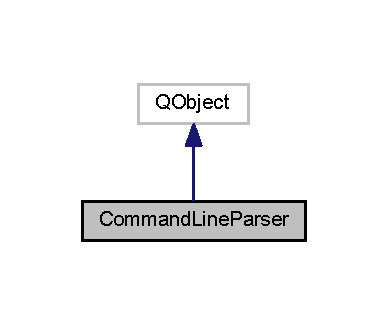
\includegraphics[width=186pt]{class_command_line_parser__inherit__graph}
\end{center}
\end{figure}


Collaboration diagram for Command\-Line\-Parser\-:
\nopagebreak
\begin{figure}[H]
\begin{center}
\leavevmode
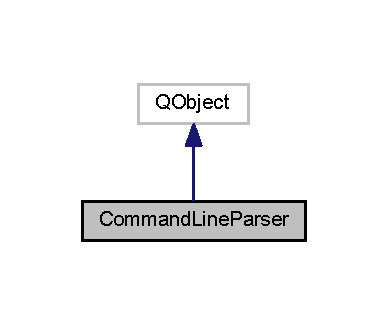
\includegraphics[width=186pt]{class_command_line_parser__coll__graph}
\end{center}
\end{figure}
\subsection*{Public Slots}
\begin{DoxyCompactItemize}
\item 
void \hyperlink{class_command_line_parser_a6a39c14ecf639b02bf8a71ac224b0a61}{Parse\-Arguments} (int argc, char $\ast$$\ast$argv)
\begin{DoxyCompactList}\small\item\em Parses the command-\/line arguments from the ignition function. \end{DoxyCompactList}\end{DoxyCompactItemize}
\subsection*{Public Member Functions}
\begin{DoxyCompactItemize}
\item 
\hyperlink{class_command_line_parser_af9c962bcd44ea242d11b88c9c28bd78d}{Command\-Line\-Parser} (Q\-Object $\ast$parent=0)
\begin{DoxyCompactList}\small\item\em Constructor. \end{DoxyCompactList}\item 
bool \hyperlink{class_command_line_parser_ac50e9de49d6e16174f6d5cf3f89c76d7}{Debugging} ()
\begin{DoxyCompactList}\small\item\em Is the application in debug mode? \end{DoxyCompactList}\item 
bool \hyperlink{class_command_line_parser_aaa2d8544c7841c33c560bb4410144154}{Logging} ()
\begin{DoxyCompactList}\small\item\em Is logging mode enabled? \end{DoxyCompactList}\end{DoxyCompactItemize}


\subsection{Detailed Description}
Deals with arguments passed to the application on the command-\/line. 

The command-\/line parser is created before the main application window is initialised and parses any options sent to the application on the command line. The global instance of the parser is made available through \hyperlink{globals_8h}{globals.\-h} under g\-\_\-p\-Cmd\-Line and several macros exist for facilitating the checking of common global application properties. See \hyperlink{globals_8h}{globals.\-h} for a full description. 

\subsection{Constructor \& Destructor Documentation}
\hypertarget{class_command_line_parser_af9c962bcd44ea242d11b88c9c28bd78d}{\index{Command\-Line\-Parser@{Command\-Line\-Parser}!Command\-Line\-Parser@{Command\-Line\-Parser}}
\index{Command\-Line\-Parser@{Command\-Line\-Parser}!CommandLineParser@{Command\-Line\-Parser}}
\subsubsection[{Command\-Line\-Parser}]{\setlength{\rightskip}{0pt plus 5cm}Command\-Line\-Parser\-::\-Command\-Line\-Parser (
\begin{DoxyParamCaption}
\item[{Q\-Object $\ast$}]{parent = {\ttfamily 0}}
\end{DoxyParamCaption}
)\hspace{0.3cm}{\ttfamily [explicit]}}}\label{class_command_line_parser_af9c962bcd44ea242d11b88c9c28bd78d}


Constructor. 


\begin{DoxyParams}{Parameters}
{\em parent} & Parent object (usually N\-U\-L\-L). \\
\hline
\end{DoxyParams}


\subsection{Member Function Documentation}
\hypertarget{class_command_line_parser_ac50e9de49d6e16174f6d5cf3f89c76d7}{\index{Command\-Line\-Parser@{Command\-Line\-Parser}!Debugging@{Debugging}}
\index{Debugging@{Debugging}!CommandLineParser@{Command\-Line\-Parser}}
\subsubsection[{Debugging}]{\setlength{\rightskip}{0pt plus 5cm}bool Command\-Line\-Parser\-::\-Debugging (
\begin{DoxyParamCaption}
{}
\end{DoxyParamCaption}
)}}\label{class_command_line_parser_ac50e9de49d6e16174f6d5cf3f89c76d7}


Is the application in debug mode? 

\begin{DoxyNote}{Note}
If enabled, the log window is available from the main application Debug menu.

If not specified, debugging mode defaults to false. 
\end{DoxyNote}
\begin{DoxyReturn}{Returns}
True if in debug mode, false otherwise. 
\end{DoxyReturn}
\hypertarget{class_command_line_parser_aaa2d8544c7841c33c560bb4410144154}{\index{Command\-Line\-Parser@{Command\-Line\-Parser}!Logging@{Logging}}
\index{Logging@{Logging}!CommandLineParser@{Command\-Line\-Parser}}
\subsubsection[{Logging}]{\setlength{\rightskip}{0pt plus 5cm}bool Command\-Line\-Parser\-::\-Logging (
\begin{DoxyParamCaption}
{}
\end{DoxyParamCaption}
)}}\label{class_command_line_parser_aaa2d8544c7841c33c560bb4410144154}


Is logging mode enabled? 

\begin{DoxyNote}{Note}
If enabled, logging messsages are written to a log file. If in debug mode, logging mode is also enabled.

If not specified, logging mode defaults to false. 
\end{DoxyNote}
\begin{DoxyReturn}{Returns}
True if enabled, false otherwise. 
\end{DoxyReturn}
\hypertarget{class_command_line_parser_a6a39c14ecf639b02bf8a71ac224b0a61}{\index{Command\-Line\-Parser@{Command\-Line\-Parser}!Parse\-Arguments@{Parse\-Arguments}}
\index{Parse\-Arguments@{Parse\-Arguments}!CommandLineParser@{Command\-Line\-Parser}}
\subsubsection[{Parse\-Arguments}]{\setlength{\rightskip}{0pt plus 5cm}void Command\-Line\-Parser\-::\-Parse\-Arguments (
\begin{DoxyParamCaption}
\item[{int}]{argc, }
\item[{char $\ast$$\ast$}]{argv}
\end{DoxyParamCaption}
)\hspace{0.3cm}{\ttfamily [slot]}}}\label{class_command_line_parser_a6a39c14ecf639b02bf8a71ac224b0a61}


Parses the command-\/line arguments from the ignition function. 


\begin{DoxyParams}{Parameters}
{\em argc} & Number of arguments. \\
\hline
{\em argv} & Char array of arguments. \\
\hline
\end{DoxyParams}


The documentation for this class was generated from the following files\-:\begin{DoxyCompactItemize}
\item 
app/\hyperlink{commandlineparser_8h}{commandlineparser.\-h}\item 
app/commandlineparser.\-cpp\end{DoxyCompactItemize}

\hypertarget{class_completion_list}{\section{Completion\-List Class Reference}
\label{class_completion_list}\index{Completion\-List@{Completion\-List}}
}


Inheritance diagram for Completion\-List\-:
\nopagebreak
\begin{figure}[H]
\begin{center}
\leavevmode
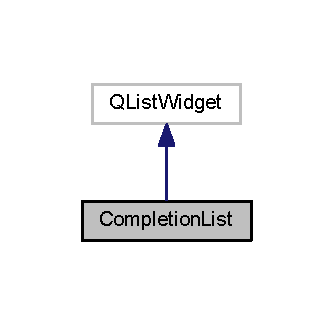
\includegraphics[width=160pt]{class_completion_list__inherit__graph}
\end{center}
\end{figure}


Collaboration diagram for Completion\-List\-:
\nopagebreak
\begin{figure}[H]
\begin{center}
\leavevmode
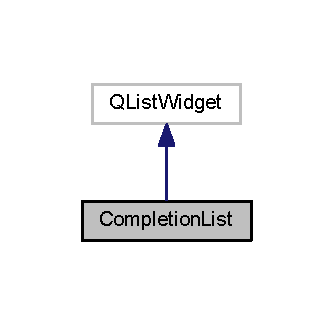
\includegraphics[width=160pt]{class_completion_list__coll__graph}
\end{center}
\end{figure}
\subsection*{Public Member Functions}
\begin{DoxyCompactItemize}
\item 
\hypertarget{class_completion_list_a034646a1bed739474eddd96ad6e2c739}{{\bfseries Completion\-List} (Q\-Widget $\ast$parent=0)}\label{class_completion_list_a034646a1bed739474eddd96ad6e2c739}

\end{DoxyCompactItemize}
\subsection*{Protected Member Functions}
\begin{DoxyCompactItemize}
\item 
\hypertarget{class_completion_list_a7be43babeb7eb4a7689aab2d03a558b9}{virtual Q\-Size {\bfseries size\-Hint} () const }\label{class_completion_list_a7be43babeb7eb4a7689aab2d03a558b9}

\item 
\hypertarget{class_completion_list_aae230c3650456c122f0740f2a2c93771}{virtual void {\bfseries key\-Press\-Event} (Q\-Key\-Event $\ast$e)}\label{class_completion_list_aae230c3650456c122f0740f2a2c93771}

\end{DoxyCompactItemize}


The documentation for this class was generated from the following files\-:\begin{DoxyCompactItemize}
\item 
I\-Console/completionlist.\-h\item 
I\-Console/completionlist.\-cpp\end{DoxyCompactItemize}

\hypertarget{class_console_window}{\section{Console\-Window Class Reference}
\label{class_console_window}\index{Console\-Window@{Console\-Window}}
}


Inheritance diagram for Console\-Window\-:
\nopagebreak
\begin{figure}[H]
\begin{center}
\leavevmode
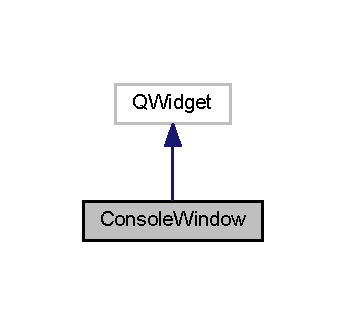
\includegraphics[width=247pt]{class_console_window__inherit__graph}
\end{center}
\end{figure}


Collaboration diagram for Console\-Window\-:
\nopagebreak
\begin{figure}[H]
\begin{center}
\leavevmode
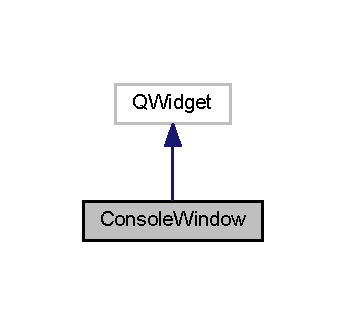
\includegraphics[width=247pt]{class_console_window__coll__graph}
\end{center}
\end{figure}
\subsection*{Public Slots}
\begin{DoxyCompactItemize}
\item 
\hypertarget{class_console_window_ae9c69bfdddc7e06686ce1aef07228a5f}{void {\bfseries slot\-Print\-Message} (const Q\-String \&message)}\label{class_console_window_ae9c69bfdddc7e06686ce1aef07228a5f}

\item 
\hypertarget{class_console_window_a2a2390460eb7eae4ba129f3e649fa03e}{void {\bfseries slot\-Print\-Warning} (const Q\-String \&message)}\label{class_console_window_a2a2390460eb7eae4ba129f3e649fa03e}

\end{DoxyCompactItemize}
\subsection*{Public Member Functions}
\begin{DoxyCompactItemize}
\item 
\hypertarget{class_console_window_a18a5ddfb71f2bcec3a4ce8abee0863eb}{{\bfseries Console\-Window} (Q\-Widget $\ast$parent=0)}\label{class_console_window_a18a5ddfb71f2bcec3a4ce8abee0863eb}

\item 
\hypertarget{class_console_window_a92eb7fb004686e2659530d959080846e}{virtual void {\bfseries print\-Message} (const Q\-String \&message)}\label{class_console_window_a92eb7fb004686e2659530d959080846e}

\item 
\hypertarget{class_console_window_ab06d210a320e402b371dfa56d73f0d54}{virtual void {\bfseries print\-Warning} (const Q\-String \&message)}\label{class_console_window_ab06d210a320e402b371dfa56d73f0d54}

\item 
\hypertarget{class_console_window_a18dbd0234d103461b57da2b724ab5b2b}{void {\bfseries set\-Warning\-Colour} (const Q\-Color col)}\label{class_console_window_a18dbd0234d103461b57da2b724ab5b2b}

\item 
\hypertarget{class_console_window_afb123596c8c2e460301721dfe28b2642}{Q\-Color {\bfseries get\-Warning\-Colour} () const }\label{class_console_window_afb123596c8c2e460301721dfe28b2642}

\item 
\hypertarget{class_console_window_a92a66819f11ee2cb7ad6079bb0542562}{void {\bfseries set\-Message\-Colour} (const Q\-Color col)}\label{class_console_window_a92a66819f11ee2cb7ad6079bb0542562}

\item 
\hypertarget{class_console_window_a4deda073bdf749e5198ba48a41fef340}{Q\-Color {\bfseries get\-Message\-Colour} () const }\label{class_console_window_a4deda073bdf749e5198ba48a41fef340}

\end{DoxyCompactItemize}


The documentation for this class was generated from the following files\-:\begin{DoxyCompactItemize}
\item 
I\-Console/consolewindow.\-h\item 
I\-Console/consolewindow.\-cpp\end{DoxyCompactItemize}

\hypertarget{class_edge3_d}{\section{Edge3\-D Class Reference}
\label{class_edge3_d}\index{Edge3\-D@{Edge3\-D}}
}


An edge links two vertices and two faces, referenced by their geometry handles.\par
 When considering travelling along the edge from the beginning to end vertex, the normals of the faces either side of the edge can be considered to point clockwise or anticlockwise around the edge. The face with an anticlockwise-\/pointing normal is denoted the \char`\"{}right\char`\"{} face (if the normal were pointing upwards the face would be positioned to the right of the edge) and the face with the clockwise-\/pointing normal is denoted the \char`\"{}left\char`\"{} face. If both normals are pointing in the same direction (either clockwise or anticlockwise) it is not defined which face is denoted left and which right.  




{\ttfamily \#include $<$edge.\-h$>$}



Inheritance diagram for Edge3\-D\-:\nopagebreak
\begin{figure}[H]
\begin{center}
\leavevmode
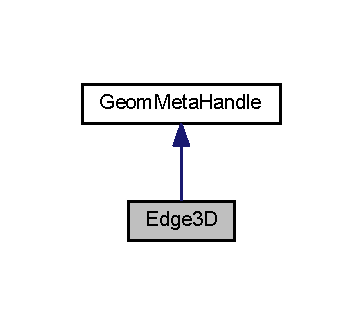
\includegraphics[width=174pt]{class_edge3_d__inherit__graph}
\end{center}
\end{figure}


Collaboration diagram for Edge3\-D\-:\nopagebreak
\begin{figure}[H]
\begin{center}
\leavevmode
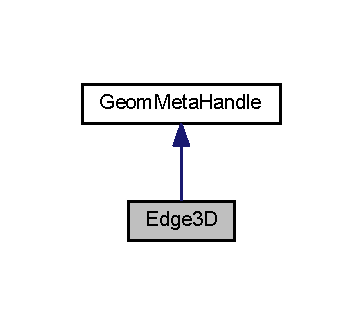
\includegraphics[width=174pt]{class_edge3_d__coll__graph}
\end{center}
\end{figure}
\subsection*{Public Member Functions}
\begin{DoxyCompactItemize}
\item 
\hypertarget{class_edge3_d_a6f25535dfee47bf06832243b11207ba6}{\hyperlink{class_edge3_d_a6f25535dfee47bf06832243b11207ba6}{Edge3\-D} ()}\label{class_edge3_d_a6f25535dfee47bf06832243b11207ba6}

\begin{DoxyCompactList}\small\item\em Constructor. Member variables are set to zero values. \end{DoxyCompactList}\item 
\hyperlink{class_edge3_d_a2c4d543fd8a4ffe272539547800c712c}{Edge3\-D} (const \hyperlink{vertex_8h_a72202e57358ed73cd212e9a2eaf39aeb}{G\-E\-O\-M\-H\-A\-N\-D\-L\-E} start, const \hyperlink{vertex_8h_a72202e57358ed73cd212e9a2eaf39aeb}{G\-E\-O\-M\-H\-A\-N\-D\-L\-E} end, const Q\-Vector3\-D midpoint)
\begin{DoxyCompactList}\small\item\em Constructor specifying start and end vertices and the midpoint of the edge. \end{DoxyCompactList}\item 
\hyperlink{class_edge3_d_af04a433a585de58702f3586d8a52219d}{Edge3\-D} (const \hyperlink{vertex_8h_a72202e57358ed73cd212e9a2eaf39aeb}{G\-E\-O\-M\-H\-A\-N\-D\-L\-E} start, const \hyperlink{vertex_8h_a72202e57358ed73cd212e9a2eaf39aeb}{G\-E\-O\-M\-H\-A\-N\-D\-L\-E} end, const \hyperlink{vertex_8h_a72202e57358ed73cd212e9a2eaf39aeb}{G\-E\-O\-M\-H\-A\-N\-D\-L\-E} rightface, const \hyperlink{vertex_8h_a72202e57358ed73cd212e9a2eaf39aeb}{G\-E\-O\-M\-H\-A\-N\-D\-L\-E} leftface, const Q\-Vector3\-D midpoint)
\begin{DoxyCompactList}\small\item\em Constructor specifying faces as well as vertices. \end{DoxyCompactList}\item 
\hyperlink{vertex_8h_a72202e57358ed73cd212e9a2eaf39aeb}{G\-E\-O\-M\-H\-A\-N\-D\-L\-E} \hyperlink{class_edge3_d_a061cf7a8c3324e564d42283702454e69}{get\-Start\-Vertex} () const 
\begin{DoxyCompactList}\small\item\em Returns the start vertex for this edge. \end{DoxyCompactList}\item 
\hyperlink{vertex_8h_a72202e57358ed73cd212e9a2eaf39aeb}{G\-E\-O\-M\-H\-A\-N\-D\-L\-E} \hyperlink{class_edge3_d_aa845b1590748b1606697afafb9b33c73}{get\-End\-Vertex} () const 
\begin{DoxyCompactList}\small\item\em Returns the end vertex of this edge. \end{DoxyCompactList}\item 
\hyperlink{vertex_8h_a72202e57358ed73cd212e9a2eaf39aeb}{G\-E\-O\-M\-H\-A\-N\-D\-L\-E} \hyperlink{class_edge3_d_a7dd9278b01fed4abf702c17eeb5c7d8b}{get\-Right\-Face} () const 
\begin{DoxyCompactList}\small\item\em Returns the edge's right face. \end{DoxyCompactList}\item 
\hyperlink{vertex_8h_a72202e57358ed73cd212e9a2eaf39aeb}{G\-E\-O\-M\-H\-A\-N\-D\-L\-E} \hyperlink{class_edge3_d_aaa398af751fda9e8b2192efef0810dc0}{get\-Left\-Face} () const 
\begin{DoxyCompactList}\small\item\em Returns the edge's left face. \end{DoxyCompactList}\item 
Q\-Vector3\-D \hyperlink{class_edge3_d_a2b97448e7bb66cf25e4bcdcff315ab5e}{get\-Midpoint} () const 
\begin{DoxyCompactList}\small\item\em Returns the edge's midpoint. \end{DoxyCompactList}\item 
\hyperlink{vertex_8h_a72202e57358ed73cd212e9a2eaf39aeb}{G\-E\-O\-M\-H\-A\-N\-D\-L\-E} \hyperlink{class_edge3_d_a34d681aaa672935753f2619ebace572b}{get\-Parent\-Solid} () const 
\begin{DoxyCompactList}\small\item\em Returns the handle of the parent solid of this edge. \end{DoxyCompactList}\item 
\hyperlink{vertex_8h_a72202e57358ed73cd212e9a2eaf39aeb}{G\-E\-O\-M\-H\-A\-N\-D\-L\-E} \hyperlink{class_edge3_d_a890650509dd10950ebaa358a349df4c7}{get\-Handle} () const 
\begin{DoxyCompactList}\small\item\em Returns this edge's geometry handle. \end{DoxyCompactList}\item 
void \hyperlink{class_edge3_d_a0533442646913ae69832e3178fa72f9a}{set\-Start\-Vertex} (const \hyperlink{vertex_8h_a72202e57358ed73cd212e9a2eaf39aeb}{G\-E\-O\-M\-H\-A\-N\-D\-L\-E} v)
\begin{DoxyCompactList}\small\item\em Sets the edge's start vertex. \end{DoxyCompactList}\item 
void \hyperlink{class_edge3_d_a32ff76ad3559822c44c8faa8519fdf74}{set\-End\-Vertex} (const \hyperlink{vertex_8h_a72202e57358ed73cd212e9a2eaf39aeb}{G\-E\-O\-M\-H\-A\-N\-D\-L\-E} v)
\begin{DoxyCompactList}\small\item\em Sets the edge's end vertex. \end{DoxyCompactList}\item 
void \hyperlink{class_edge3_d_a9960f64e5fceb5a6dc828893fe704cb6}{set\-Right\-Face} (const \hyperlink{vertex_8h_a72202e57358ed73cd212e9a2eaf39aeb}{G\-E\-O\-M\-H\-A\-N\-D\-L\-E} f)
\begin{DoxyCompactList}\small\item\em Sets the edge's right face. \end{DoxyCompactList}\item 
void \hyperlink{class_edge3_d_a1d87d3eed968ddce326ac07cc7c98e34}{set\-Left\-Face} (const \hyperlink{vertex_8h_a72202e57358ed73cd212e9a2eaf39aeb}{G\-E\-O\-M\-H\-A\-N\-D\-L\-E} f)
\begin{DoxyCompactList}\small\item\em Sets the edge's left face. \end{DoxyCompactList}\item 
void \hyperlink{class_edge3_d_a5b5e77a0d19f391cf987510111bc32f6}{set\-Midpoint} (const Q\-Vector3\-D mid)
\begin{DoxyCompactList}\small\item\em Sets the edge's midpoint. \end{DoxyCompactList}\item 
void \hyperlink{class_edge3_d_ad905287b0350a41fcf82c638e247255c}{set\-Parent\-Solid} (const \hyperlink{vertex_8h_a72202e57358ed73cd212e9a2eaf39aeb}{G\-E\-O\-M\-H\-A\-N\-D\-L\-E} handle)
\begin{DoxyCompactList}\small\item\em Sets the parent solid handle for this edge. \end{DoxyCompactList}\item 
void \hyperlink{class_edge3_d_a7ad6b919f69ee151ce78a3d5d2b41096}{set\-Handle} (const \hyperlink{vertex_8h_a72202e57358ed73cd212e9a2eaf39aeb}{G\-E\-O\-M\-H\-A\-N\-D\-L\-E} handle)
\begin{DoxyCompactList}\small\item\em Sets this edge's handle. \end{DoxyCompactList}\item 
bool \hyperlink{class_edge3_d_a9cd240bf4c0f68b3085777935e11fb85}{calc\-Midpoint} (\hyperlink{class_solid3_d}{Solid3\-D} \&parent)
\begin{DoxyCompactList}\small\item\em Given a parent solid, calculates the mid-\/point of the edge by looking up the vertices it references. \end{DoxyCompactList}\end{DoxyCompactItemize}
\subsection*{Additional Inherited Members}


\subsection{Detailed Description}
An edge links two vertices and two faces, referenced by their geometry handles.\par
 When considering travelling along the edge from the beginning to end vertex, the normals of the faces either side of the edge can be considered to point clockwise or anticlockwise around the edge. The face with an anticlockwise-\/pointing normal is denoted the \char`\"{}right\char`\"{} face (if the normal were pointing upwards the face would be positioned to the right of the edge) and the face with the clockwise-\/pointing normal is denoted the \char`\"{}left\char`\"{} face. If both normals are pointing in the same direction (either clockwise or anticlockwise) it is not defined which face is denoted left and which right. 

\subsection{Constructor \& Destructor Documentation}
\hypertarget{class_edge3_d_a2c4d543fd8a4ffe272539547800c712c}{\index{Edge3\-D@{Edge3\-D}!Edge3\-D@{Edge3\-D}}
\index{Edge3\-D@{Edge3\-D}!Edge3D@{Edge3\-D}}
\subsubsection[{Edge3\-D}]{\setlength{\rightskip}{0pt plus 5cm}Edge3\-D\-::\-Edge3\-D (
\begin{DoxyParamCaption}
\item[{const {\bf G\-E\-O\-M\-H\-A\-N\-D\-L\-E}}]{start, }
\item[{const {\bf G\-E\-O\-M\-H\-A\-N\-D\-L\-E}}]{end, }
\item[{const Q\-Vector3\-D}]{midpoint}
\end{DoxyParamCaption}
)\hspace{0.3cm}{\ttfamily [inline]}}}\label{class_edge3_d_a2c4d543fd8a4ffe272539547800c712c}


Constructor specifying start and end vertices and the midpoint of the edge. 


\begin{DoxyParams}{Parameters}
{\em start} & I\-D of vertex this edge starts at. \\
\hline
{\em end} & I\-D of vertex this edge ends at. \\
\hline
{\em midpoint} & Co-\/ordinates of the edge's midpoint. \\
\hline
\end{DoxyParams}
\hypertarget{class_edge3_d_af04a433a585de58702f3586d8a52219d}{\index{Edge3\-D@{Edge3\-D}!Edge3\-D@{Edge3\-D}}
\index{Edge3\-D@{Edge3\-D}!Edge3D@{Edge3\-D}}
\subsubsection[{Edge3\-D}]{\setlength{\rightskip}{0pt plus 5cm}Edge3\-D\-::\-Edge3\-D (
\begin{DoxyParamCaption}
\item[{const {\bf G\-E\-O\-M\-H\-A\-N\-D\-L\-E}}]{start, }
\item[{const {\bf G\-E\-O\-M\-H\-A\-N\-D\-L\-E}}]{end, }
\item[{const {\bf G\-E\-O\-M\-H\-A\-N\-D\-L\-E}}]{rightface, }
\item[{const {\bf G\-E\-O\-M\-H\-A\-N\-D\-L\-E}}]{leftface, }
\item[{const Q\-Vector3\-D}]{midpoint}
\end{DoxyParamCaption}
)\hspace{0.3cm}{\ttfamily [inline]}}}\label{class_edge3_d_af04a433a585de58702f3586d8a52219d}


Constructor specifying faces as well as vertices. 


\begin{DoxyParams}{Parameters}
{\em start} & I\-D of vertex this edge starts at. \\
\hline
{\em end} & I\-D of vertex this edge ends at. \\
\hline
{\em rightface} & Face to the right of this edge (see page description). \\
\hline
{\em leftface} & Face to the left of this edge (see page description). \\
\hline
{\em midpoint} & Co-\/ordinates of the edge's midpoint. \\
\hline
\end{DoxyParams}


\subsection{Member Function Documentation}
\hypertarget{class_edge3_d_a9cd240bf4c0f68b3085777935e11fb85}{\index{Edge3\-D@{Edge3\-D}!calc\-Midpoint@{calc\-Midpoint}}
\index{calc\-Midpoint@{calc\-Midpoint}!Edge3D@{Edge3\-D}}
\subsubsection[{calc\-Midpoint}]{\setlength{\rightskip}{0pt plus 5cm}bool Edge3\-D\-::calc\-Midpoint (
\begin{DoxyParamCaption}
\item[{{\bf Solid3\-D} \&}]{parent}
\end{DoxyParamCaption}
)}}\label{class_edge3_d_a9cd240bf4c0f68b3085777935e11fb85}


Given a parent solid, calculates the mid-\/point of the edge by looking up the vertices it references. 


\begin{DoxyParams}{Parameters}
{\em parent} & Parent solid of this edge. \\
\hline
\end{DoxyParams}
\hypertarget{class_edge3_d_aa845b1590748b1606697afafb9b33c73}{\index{Edge3\-D@{Edge3\-D}!get\-End\-Vertex@{get\-End\-Vertex}}
\index{get\-End\-Vertex@{get\-End\-Vertex}!Edge3D@{Edge3\-D}}
\subsubsection[{get\-End\-Vertex}]{\setlength{\rightskip}{0pt plus 5cm}{\bf G\-E\-O\-M\-H\-A\-N\-D\-L\-E} Edge3\-D\-::get\-End\-Vertex (
\begin{DoxyParamCaption}
{}
\end{DoxyParamCaption}
) const\hspace{0.3cm}{\ttfamily [inline]}}}\label{class_edge3_d_aa845b1590748b1606697afafb9b33c73}


Returns the end vertex of this edge. 

\begin{DoxyReturn}{Returns}
End vertex I\-D. 
\end{DoxyReturn}
\hypertarget{class_edge3_d_a890650509dd10950ebaa358a349df4c7}{\index{Edge3\-D@{Edge3\-D}!get\-Handle@{get\-Handle}}
\index{get\-Handle@{get\-Handle}!Edge3D@{Edge3\-D}}
\subsubsection[{get\-Handle}]{\setlength{\rightskip}{0pt plus 5cm}{\bf G\-E\-O\-M\-H\-A\-N\-D\-L\-E} Edge3\-D\-::get\-Handle (
\begin{DoxyParamCaption}
{}
\end{DoxyParamCaption}
) const\hspace{0.3cm}{\ttfamily [inline]}}}\label{class_edge3_d_a890650509dd10950ebaa358a349df4c7}


Returns this edge's geometry handle. 

\begin{DoxyReturn}{Returns}
Handle for this edge. 
\end{DoxyReturn}
\hypertarget{class_edge3_d_aaa398af751fda9e8b2192efef0810dc0}{\index{Edge3\-D@{Edge3\-D}!get\-Left\-Face@{get\-Left\-Face}}
\index{get\-Left\-Face@{get\-Left\-Face}!Edge3D@{Edge3\-D}}
\subsubsection[{get\-Left\-Face}]{\setlength{\rightskip}{0pt plus 5cm}{\bf G\-E\-O\-M\-H\-A\-N\-D\-L\-E} Edge3\-D\-::get\-Left\-Face (
\begin{DoxyParamCaption}
{}
\end{DoxyParamCaption}
) const\hspace{0.3cm}{\ttfamily [inline]}}}\label{class_edge3_d_aaa398af751fda9e8b2192efef0810dc0}


Returns the edge's left face. 

\begin{DoxyReturn}{Returns}
Left face I\-D (see page description). 
\end{DoxyReturn}
\hypertarget{class_edge3_d_a2b97448e7bb66cf25e4bcdcff315ab5e}{\index{Edge3\-D@{Edge3\-D}!get\-Midpoint@{get\-Midpoint}}
\index{get\-Midpoint@{get\-Midpoint}!Edge3D@{Edge3\-D}}
\subsubsection[{get\-Midpoint}]{\setlength{\rightskip}{0pt plus 5cm}Q\-Vector3\-D Edge3\-D\-::get\-Midpoint (
\begin{DoxyParamCaption}
{}
\end{DoxyParamCaption}
) const\hspace{0.3cm}{\ttfamily [inline]}}}\label{class_edge3_d_a2b97448e7bb66cf25e4bcdcff315ab5e}


Returns the edge's midpoint. 

\begin{DoxyReturn}{Returns}
Co-\/ordinates of midpoint of edge. 
\end{DoxyReturn}
\hypertarget{class_edge3_d_a34d681aaa672935753f2619ebace572b}{\index{Edge3\-D@{Edge3\-D}!get\-Parent\-Solid@{get\-Parent\-Solid}}
\index{get\-Parent\-Solid@{get\-Parent\-Solid}!Edge3D@{Edge3\-D}}
\subsubsection[{get\-Parent\-Solid}]{\setlength{\rightskip}{0pt plus 5cm}{\bf G\-E\-O\-M\-H\-A\-N\-D\-L\-E} Edge3\-D\-::get\-Parent\-Solid (
\begin{DoxyParamCaption}
{}
\end{DoxyParamCaption}
) const\hspace{0.3cm}{\ttfamily [inline]}}}\label{class_edge3_d_a34d681aaa672935753f2619ebace572b}


Returns the handle of the parent solid of this edge. 

\begin{DoxyReturn}{Returns}
Parent solid handle. 
\end{DoxyReturn}
\hypertarget{class_edge3_d_a7dd9278b01fed4abf702c17eeb5c7d8b}{\index{Edge3\-D@{Edge3\-D}!get\-Right\-Face@{get\-Right\-Face}}
\index{get\-Right\-Face@{get\-Right\-Face}!Edge3D@{Edge3\-D}}
\subsubsection[{get\-Right\-Face}]{\setlength{\rightskip}{0pt plus 5cm}{\bf G\-E\-O\-M\-H\-A\-N\-D\-L\-E} Edge3\-D\-::get\-Right\-Face (
\begin{DoxyParamCaption}
{}
\end{DoxyParamCaption}
) const\hspace{0.3cm}{\ttfamily [inline]}}}\label{class_edge3_d_a7dd9278b01fed4abf702c17eeb5c7d8b}


Returns the edge's right face. 

\begin{DoxyReturn}{Returns}
Right face I\-D (see page description). 
\end{DoxyReturn}
\hypertarget{class_edge3_d_a061cf7a8c3324e564d42283702454e69}{\index{Edge3\-D@{Edge3\-D}!get\-Start\-Vertex@{get\-Start\-Vertex}}
\index{get\-Start\-Vertex@{get\-Start\-Vertex}!Edge3D@{Edge3\-D}}
\subsubsection[{get\-Start\-Vertex}]{\setlength{\rightskip}{0pt plus 5cm}{\bf G\-E\-O\-M\-H\-A\-N\-D\-L\-E} Edge3\-D\-::get\-Start\-Vertex (
\begin{DoxyParamCaption}
{}
\end{DoxyParamCaption}
) const\hspace{0.3cm}{\ttfamily [inline]}}}\label{class_edge3_d_a061cf7a8c3324e564d42283702454e69}


Returns the start vertex for this edge. 

\begin{DoxyReturn}{Returns}
Start vertex I\-D. 
\end{DoxyReturn}
\hypertarget{class_edge3_d_a32ff76ad3559822c44c8faa8519fdf74}{\index{Edge3\-D@{Edge3\-D}!set\-End\-Vertex@{set\-End\-Vertex}}
\index{set\-End\-Vertex@{set\-End\-Vertex}!Edge3D@{Edge3\-D}}
\subsubsection[{set\-End\-Vertex}]{\setlength{\rightskip}{0pt plus 5cm}void Edge3\-D\-::set\-End\-Vertex (
\begin{DoxyParamCaption}
\item[{const {\bf G\-E\-O\-M\-H\-A\-N\-D\-L\-E}}]{v}
\end{DoxyParamCaption}
)\hspace{0.3cm}{\ttfamily [inline]}}}\label{class_edge3_d_a32ff76ad3559822c44c8faa8519fdf74}


Sets the edge's end vertex. 


\begin{DoxyParams}{Parameters}
{\em v} & Vertex I\-D to set. \\
\hline
\end{DoxyParams}
\hypertarget{class_edge3_d_a7ad6b919f69ee151ce78a3d5d2b41096}{\index{Edge3\-D@{Edge3\-D}!set\-Handle@{set\-Handle}}
\index{set\-Handle@{set\-Handle}!Edge3D@{Edge3\-D}}
\subsubsection[{set\-Handle}]{\setlength{\rightskip}{0pt plus 5cm}void Edge3\-D\-::set\-Handle (
\begin{DoxyParamCaption}
\item[{const {\bf G\-E\-O\-M\-H\-A\-N\-D\-L\-E}}]{handle}
\end{DoxyParamCaption}
)\hspace{0.3cm}{\ttfamily [inline]}}}\label{class_edge3_d_a7ad6b919f69ee151ce78a3d5d2b41096}


Sets this edge's handle. 


\begin{DoxyParams}{Parameters}
{\em handle} & Handle to set. \\
\hline
\end{DoxyParams}
\hypertarget{class_edge3_d_a1d87d3eed968ddce326ac07cc7c98e34}{\index{Edge3\-D@{Edge3\-D}!set\-Left\-Face@{set\-Left\-Face}}
\index{set\-Left\-Face@{set\-Left\-Face}!Edge3D@{Edge3\-D}}
\subsubsection[{set\-Left\-Face}]{\setlength{\rightskip}{0pt plus 5cm}void Edge3\-D\-::set\-Left\-Face (
\begin{DoxyParamCaption}
\item[{const {\bf G\-E\-O\-M\-H\-A\-N\-D\-L\-E}}]{f}
\end{DoxyParamCaption}
)\hspace{0.3cm}{\ttfamily [inline]}}}\label{class_edge3_d_a1d87d3eed968ddce326ac07cc7c98e34}


Sets the edge's left face. 


\begin{DoxyParams}{Parameters}
{\em f} & Face I\-D to set. \\
\hline
\end{DoxyParams}
\hypertarget{class_edge3_d_a5b5e77a0d19f391cf987510111bc32f6}{\index{Edge3\-D@{Edge3\-D}!set\-Midpoint@{set\-Midpoint}}
\index{set\-Midpoint@{set\-Midpoint}!Edge3D@{Edge3\-D}}
\subsubsection[{set\-Midpoint}]{\setlength{\rightskip}{0pt plus 5cm}void Edge3\-D\-::set\-Midpoint (
\begin{DoxyParamCaption}
\item[{const Q\-Vector3\-D}]{mid}
\end{DoxyParamCaption}
)\hspace{0.3cm}{\ttfamily [inline]}}}\label{class_edge3_d_a5b5e77a0d19f391cf987510111bc32f6}


Sets the edge's midpoint. 


\begin{DoxyParams}{Parameters}
{\em mid} & Co-\/ordinates of midpoint. \\
\hline
\end{DoxyParams}
\hypertarget{class_edge3_d_ad905287b0350a41fcf82c638e247255c}{\index{Edge3\-D@{Edge3\-D}!set\-Parent\-Solid@{set\-Parent\-Solid}}
\index{set\-Parent\-Solid@{set\-Parent\-Solid}!Edge3D@{Edge3\-D}}
\subsubsection[{set\-Parent\-Solid}]{\setlength{\rightskip}{0pt plus 5cm}void Edge3\-D\-::set\-Parent\-Solid (
\begin{DoxyParamCaption}
\item[{const {\bf G\-E\-O\-M\-H\-A\-N\-D\-L\-E}}]{handle}
\end{DoxyParamCaption}
)\hspace{0.3cm}{\ttfamily [inline]}}}\label{class_edge3_d_ad905287b0350a41fcf82c638e247255c}


Sets the parent solid handle for this edge. 


\begin{DoxyParams}{Parameters}
{\em handle} & Handle to set. \\
\hline
\end{DoxyParams}
\hypertarget{class_edge3_d_a9960f64e5fceb5a6dc828893fe704cb6}{\index{Edge3\-D@{Edge3\-D}!set\-Right\-Face@{set\-Right\-Face}}
\index{set\-Right\-Face@{set\-Right\-Face}!Edge3D@{Edge3\-D}}
\subsubsection[{set\-Right\-Face}]{\setlength{\rightskip}{0pt plus 5cm}void Edge3\-D\-::set\-Right\-Face (
\begin{DoxyParamCaption}
\item[{const {\bf G\-E\-O\-M\-H\-A\-N\-D\-L\-E}}]{f}
\end{DoxyParamCaption}
)\hspace{0.3cm}{\ttfamily [inline]}}}\label{class_edge3_d_a9960f64e5fceb5a6dc828893fe704cb6}


Sets the edge's right face. 


\begin{DoxyParams}{Parameters}
{\em f} & Face I\-D to set. \\
\hline
\end{DoxyParams}
\hypertarget{class_edge3_d_a0533442646913ae69832e3178fa72f9a}{\index{Edge3\-D@{Edge3\-D}!set\-Start\-Vertex@{set\-Start\-Vertex}}
\index{set\-Start\-Vertex@{set\-Start\-Vertex}!Edge3D@{Edge3\-D}}
\subsubsection[{set\-Start\-Vertex}]{\setlength{\rightskip}{0pt plus 5cm}void Edge3\-D\-::set\-Start\-Vertex (
\begin{DoxyParamCaption}
\item[{const {\bf G\-E\-O\-M\-H\-A\-N\-D\-L\-E}}]{v}
\end{DoxyParamCaption}
)\hspace{0.3cm}{\ttfamily [inline]}}}\label{class_edge3_d_a0533442646913ae69832e3178fa72f9a}


Sets the edge's start vertex. 


\begin{DoxyParams}{Parameters}
{\em v} & Vertex I\-D to set. \\
\hline
\end{DoxyParams}


The documentation for this class was generated from the following files\-:\begin{DoxyCompactItemize}
\item 
app/\hyperlink{edge_8h}{edge.\-h}\item 
app/edge.\-cpp\end{DoxyCompactItemize}

\hypertarget{class_face3_d}{\section{Face3\-D Class Reference}
\label{class_face3_d}\index{Face3\-D@{Face3\-D}}
}


Class representing a 3\-D face.  




{\ttfamily \#include $<$face.\-h$>$}



Inheritance diagram for Face3\-D\-:
\nopagebreak
\begin{figure}[H]
\begin{center}
\leavevmode
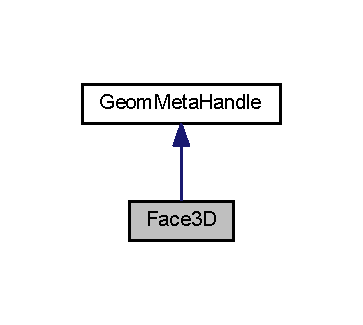
\includegraphics[width=174pt]{class_face3_d__inherit__graph}
\end{center}
\end{figure}


Collaboration diagram for Face3\-D\-:
\nopagebreak
\begin{figure}[H]
\begin{center}
\leavevmode
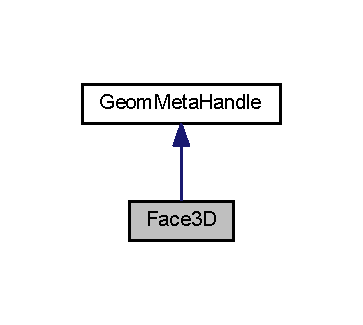
\includegraphics[width=174pt]{class_face3_d__coll__graph}
\end{center}
\end{figure}
\subsection*{Public Member Functions}
\begin{DoxyCompactItemize}
\item 
\hypertarget{class_face3_d_af64a4a5fe2a8f06dd684bff91041e0cb}{\hyperlink{class_face3_d_af64a4a5fe2a8f06dd684bff91041e0cb}{Face3\-D} ()}\label{class_face3_d_af64a4a5fe2a8f06dd684bff91041e0cb}

\begin{DoxyCompactList}\small\item\em Constructor. Sets member variables to default values. \end{DoxyCompactList}\item 
\hyperlink{class_face3_d_a6113068475ee9edc57445f8eac3d4f5b}{Face3\-D} (const \hyperlink{class_plane}{Plane} p, const Q\-Vector3\-D centre=\hyperlink{matlib_8h_ac2de4dab97258eff87e0a1253a2d1a29}{V\-E\-C3\-\_\-\-O\-R\-I\-G\-I\-N})
\begin{DoxyCompactList}\small\item\em Constructor specifying plane and centre point of face. \end{DoxyCompactList}\item 
\hypertarget{class_face3_d_af7dc0f5eb3359689d7617cad7fe65797}{\hyperlink{class_face3_d_af7dc0f5eb3359689d7617cad7fe65797}{$\sim$\-Face3\-D} ()}\label{class_face3_d_af7dc0f5eb3359689d7617cad7fe65797}

\begin{DoxyCompactList}\small\item\em Destructor. \end{DoxyCompactList}\item 
int \hyperlink{class_face3_d_a83db8beee23e03ff24cd9b0649e8269c}{get\-Edge\-Count} () const 
\begin{DoxyCompactList}\small\item\em Returns the number of edges this face contains. \end{DoxyCompactList}\item 
\hyperlink{vertex_8h_a72202e57358ed73cd212e9a2eaf39aeb}{G\-E\-O\-M\-H\-A\-N\-D\-L\-E} \hyperlink{class_face3_d_a7a44b794e450e4e9784484876e10710b}{get\-Edge\-Handle} (const int index) const 
\begin{DoxyCompactList}\small\item\em Returns the handle to the edge at a specific index in the edge list. Index must be within range. \end{DoxyCompactList}\item 
\hyperlink{class_plane}{Plane} \hyperlink{class_face3_d_a1e3d068cffc33876100a3affc496e8eb}{get\-Plane} () const 
\begin{DoxyCompactList}\small\item\em Gets the plane that represents this face's surface. \end{DoxyCompactList}\item 
Q\-Vector3\-D \hyperlink{class_face3_d_a0dfbcd5b1fa9fd18d2b09064d5dff8ac}{get\-Normal} () const 
\begin{DoxyCompactList}\small\item\em Gets this face's normal. \end{DoxyCompactList}\item 
bool \hyperlink{class_face3_d_a9e8a8bcd2337cc8aeaa231aba7c5996b}{is\-Plane\-Valid} () const 
\begin{DoxyCompactList}\small\item\em Returns whether the face's plane is valid. \end{DoxyCompactList}\item 
Q\-Vector3\-D \hyperlink{class_face3_d_a34bc3d8aeb903d18d3f05b6af299fdff}{get\-Centre\-Point} () const 
\begin{DoxyCompactList}\small\item\em Gets the central point of the face. \end{DoxyCompactList}\item 
\hyperlink{vertex_8h_a72202e57358ed73cd212e9a2eaf39aeb}{G\-E\-O\-M\-H\-A\-N\-D\-L\-E} \hyperlink{class_face3_d_a84bf13a7355baeeedf35b6da66c064ec}{get\-Parent\-Solid} () const 
\begin{DoxyCompactList}\small\item\em Gets the hand of the parent solid of this face. \end{DoxyCompactList}\item 
\hyperlink{vertex_8h_a72202e57358ed73cd212e9a2eaf39aeb}{G\-E\-O\-M\-H\-A\-N\-D\-L\-E} \hyperlink{class_face3_d_ad0bc376833756ff964ad8967fc459c8f}{get\-Handle} () const 
\begin{DoxyCompactList}\small\item\em Gets this face's handle. \end{DoxyCompactList}\item 
bool \hyperlink{class_face3_d_a7b6289ce08b7e07e050641449d42a4d7}{contains\-Edge} (const \hyperlink{vertex_8h_a72202e57358ed73cd212e9a2eaf39aeb}{G\-E\-O\-M\-H\-A\-N\-D\-L\-E} edge) const 
\begin{DoxyCompactList}\small\item\em Returns whether this face contains an edge with the specified handle. \end{DoxyCompactList}\item 
bool \hyperlink{class_face3_d_ae8daf489ffc7b411edb78b2e62e95e80}{contains\-Any\-Edge} (const Q\-List$<$ \hyperlink{vertex_8h_a72202e57358ed73cd212e9a2eaf39aeb}{G\-E\-O\-M\-H\-A\-N\-D\-L\-E} $>$ \&edges) const 
\begin{DoxyCompactList}\small\item\em Returns whether this face contains any of the edges in the list provided. \end{DoxyCompactList}\item 
void \hyperlink{class_face3_d_ab58095c8043c2f08751327a6399365c9}{set\-Plane} (const \hyperlink{class_plane}{Plane} p)
\begin{DoxyCompactList}\small\item\em Set's the face's plane. \end{DoxyCompactList}\item 
void \hyperlink{class_face3_d_aedb4458bdb3b06dddd830c53726aa844}{set\-Centre\-Point} (const Q\-Vector3\-D centre)
\begin{DoxyCompactList}\small\item\em Sets the face's central point. \end{DoxyCompactList}\item 
void \hyperlink{class_face3_d_aaf0b823d7e83800962181136a3806be5}{set\-Parent\-Solid} (const \hyperlink{vertex_8h_a72202e57358ed73cd212e9a2eaf39aeb}{G\-E\-O\-M\-H\-A\-N\-D\-L\-E} handle)
\begin{DoxyCompactList}\small\item\em Sets the parent solid handle for this face. \end{DoxyCompactList}\item 
void \hyperlink{class_face3_d_a3f040832e7d61cddc9286acce1597bfd}{set\-Handle} (const \hyperlink{vertex_8h_a72202e57358ed73cd212e9a2eaf39aeb}{G\-E\-O\-M\-H\-A\-N\-D\-L\-E} handle)
\begin{DoxyCompactList}\small\item\em Sets the handle of this face. \end{DoxyCompactList}\item 
void \hyperlink{class_face3_d_a67c54bddb563a26bdde53b59ba38ae86}{add\-Edge} (\hyperlink{vertex_8h_a72202e57358ed73cd212e9a2eaf39aeb}{G\-E\-O\-M\-H\-A\-N\-D\-L\-E} edge)
\begin{DoxyCompactList}\small\item\em Adds an edge to this face. The edge must already exist in the face's parent solid. \end{DoxyCompactList}\item 
bool \hyperlink{class_face3_d_a5f360979f999dfaa2f7be7ed3c66ef0f}{is\-Composite} ()
\begin{DoxyCompactList}\small\item\em Returns whether the face is composite. Composite faces contain more than just three edges (ie. they are composed of more than one triangle). \end{DoxyCompactList}\end{DoxyCompactItemize}
\subsection*{Additional Inherited Members}


\subsection{Detailed Description}
Class representing a 3\-D face. 

Solids are made up of faces, which are built up from lists of member edges. Faces also contain plane information (for easy conversion to/from V\-M\-Fs). The direction of the face's edges according to their start/end vertices does not necessarily have to be clockwise (this would be impractical) but the edges do have to form a closed, contiguous loop from the beginning to the end of the list, the last vertex of the last edge being the first vertex of the first edge. The loop should form a convex 2\-D polygon. 

\subsection{Constructor \& Destructor Documentation}
\hypertarget{class_face3_d_a6113068475ee9edc57445f8eac3d4f5b}{\index{Face3\-D@{Face3\-D}!Face3\-D@{Face3\-D}}
\index{Face3\-D@{Face3\-D}!Face3D@{Face3\-D}}
\subsubsection[{Face3\-D}]{\setlength{\rightskip}{0pt plus 5cm}Face3\-D\-::\-Face3\-D (
\begin{DoxyParamCaption}
\item[{const {\bf Plane}}]{p, }
\item[{const Q\-Vector3\-D}]{centre = {\ttfamily {\bf V\-E\-C3\-\_\-\-O\-R\-I\-G\-I\-N}}}
\end{DoxyParamCaption}
)\hspace{0.3cm}{\ttfamily [inline]}}}\label{class_face3_d_a6113068475ee9edc57445f8eac3d4f5b}


Constructor specifying plane and centre point of face. 


\begin{DoxyParams}{Parameters}
{\em p} & \\
\hline
{\em centre} & \\
\hline
\end{DoxyParams}


\subsection{Member Function Documentation}
\hypertarget{class_face3_d_a67c54bddb563a26bdde53b59ba38ae86}{\index{Face3\-D@{Face3\-D}!add\-Edge@{add\-Edge}}
\index{add\-Edge@{add\-Edge}!Face3D@{Face3\-D}}
\subsubsection[{add\-Edge}]{\setlength{\rightskip}{0pt plus 5cm}void Face3\-D\-::add\-Edge (
\begin{DoxyParamCaption}
\item[{{\bf G\-E\-O\-M\-H\-A\-N\-D\-L\-E}}]{edge}
\end{DoxyParamCaption}
)\hspace{0.3cm}{\ttfamily [inline]}}}\label{class_face3_d_a67c54bddb563a26bdde53b59ba38ae86}


Adds an edge to this face. The edge must already exist in the face's parent solid. 

\begin{DoxyNote}{Note}
Does N\-O\-T check whether the edge already exists in the face. 
\end{DoxyNote}

\begin{DoxyParams}{Parameters}
{\em edge} & Handle of the edge to add. \\
\hline
\end{DoxyParams}
\hypertarget{class_face3_d_ae8daf489ffc7b411edb78b2e62e95e80}{\index{Face3\-D@{Face3\-D}!contains\-Any\-Edge@{contains\-Any\-Edge}}
\index{contains\-Any\-Edge@{contains\-Any\-Edge}!Face3D@{Face3\-D}}
\subsubsection[{contains\-Any\-Edge}]{\setlength{\rightskip}{0pt plus 5cm}bool Face3\-D\-::contains\-Any\-Edge (
\begin{DoxyParamCaption}
\item[{const Q\-List$<$ {\bf G\-E\-O\-M\-H\-A\-N\-D\-L\-E} $>$ \&}]{edges}
\end{DoxyParamCaption}
) const}}\label{class_face3_d_ae8daf489ffc7b411edb78b2e62e95e80}


Returns whether this face contains any of the edges in the list provided. 


\begin{DoxyParams}{Parameters}
{\em edges} & List of edge handles to check. \\
\hline
\end{DoxyParams}
\begin{DoxyReturn}{Returns}
True if the face contains any edge, false if the face contains none of the edges. 
\end{DoxyReturn}
\hypertarget{class_face3_d_a7b6289ce08b7e07e050641449d42a4d7}{\index{Face3\-D@{Face3\-D}!contains\-Edge@{contains\-Edge}}
\index{contains\-Edge@{contains\-Edge}!Face3D@{Face3\-D}}
\subsubsection[{contains\-Edge}]{\setlength{\rightskip}{0pt plus 5cm}bool Face3\-D\-::contains\-Edge (
\begin{DoxyParamCaption}
\item[{const {\bf G\-E\-O\-M\-H\-A\-N\-D\-L\-E}}]{edge}
\end{DoxyParamCaption}
) const}}\label{class_face3_d_a7b6289ce08b7e07e050641449d42a4d7}


Returns whether this face contains an edge with the specified handle. 


\begin{DoxyParams}{Parameters}
{\em edge} & Handle to check. \\
\hline
\end{DoxyParams}
\begin{DoxyReturn}{Returns}
True if the edge is contained within the face, false if not. 
\end{DoxyReturn}
\hypertarget{class_face3_d_a34bc3d8aeb903d18d3f05b6af299fdff}{\index{Face3\-D@{Face3\-D}!get\-Centre\-Point@{get\-Centre\-Point}}
\index{get\-Centre\-Point@{get\-Centre\-Point}!Face3D@{Face3\-D}}
\subsubsection[{get\-Centre\-Point}]{\setlength{\rightskip}{0pt plus 5cm}Q\-Vector3\-D Face3\-D\-::get\-Centre\-Point (
\begin{DoxyParamCaption}
{}
\end{DoxyParamCaption}
) const\hspace{0.3cm}{\ttfamily [inline]}}}\label{class_face3_d_a34bc3d8aeb903d18d3f05b6af299fdff}


Gets the central point of the face. 

\begin{DoxyReturn}{Returns}
Face centre point. 
\end{DoxyReturn}
\hypertarget{class_face3_d_a83db8beee23e03ff24cd9b0649e8269c}{\index{Face3\-D@{Face3\-D}!get\-Edge\-Count@{get\-Edge\-Count}}
\index{get\-Edge\-Count@{get\-Edge\-Count}!Face3D@{Face3\-D}}
\subsubsection[{get\-Edge\-Count}]{\setlength{\rightskip}{0pt plus 5cm}int Face3\-D\-::get\-Edge\-Count (
\begin{DoxyParamCaption}
{}
\end{DoxyParamCaption}
) const\hspace{0.3cm}{\ttfamily [inline]}}}\label{class_face3_d_a83db8beee23e03ff24cd9b0649e8269c}


Returns the number of edges this face contains. 

\begin{DoxyReturn}{Returns}
Number of edges. 
\end{DoxyReturn}
\hypertarget{class_face3_d_a7a44b794e450e4e9784484876e10710b}{\index{Face3\-D@{Face3\-D}!get\-Edge\-Handle@{get\-Edge\-Handle}}
\index{get\-Edge\-Handle@{get\-Edge\-Handle}!Face3D@{Face3\-D}}
\subsubsection[{get\-Edge\-Handle}]{\setlength{\rightskip}{0pt plus 5cm}{\bf G\-E\-O\-M\-H\-A\-N\-D\-L\-E} Face3\-D\-::get\-Edge\-Handle (
\begin{DoxyParamCaption}
\item[{const int}]{index}
\end{DoxyParamCaption}
) const\hspace{0.3cm}{\ttfamily [inline]}}}\label{class_face3_d_a7a44b794e450e4e9784484876e10710b}


Returns the handle to the edge at a specific index in the edge list. Index must be within range. 


\begin{DoxyParams}{Parameters}
{\em index} & Index of edge to retrieve. \\
\hline
\end{DoxyParams}
\begin{DoxyReturn}{Returns}
Edge at this index. 
\end{DoxyReturn}
\hypertarget{class_face3_d_ad0bc376833756ff964ad8967fc459c8f}{\index{Face3\-D@{Face3\-D}!get\-Handle@{get\-Handle}}
\index{get\-Handle@{get\-Handle}!Face3D@{Face3\-D}}
\subsubsection[{get\-Handle}]{\setlength{\rightskip}{0pt plus 5cm}{\bf G\-E\-O\-M\-H\-A\-N\-D\-L\-E} Face3\-D\-::get\-Handle (
\begin{DoxyParamCaption}
{}
\end{DoxyParamCaption}
) const\hspace{0.3cm}{\ttfamily [inline]}}}\label{class_face3_d_ad0bc376833756ff964ad8967fc459c8f}


Gets this face's handle. 

\begin{DoxyReturn}{Returns}
Handle of the face. 
\end{DoxyReturn}
\hypertarget{class_face3_d_a0dfbcd5b1fa9fd18d2b09064d5dff8ac}{\index{Face3\-D@{Face3\-D}!get\-Normal@{get\-Normal}}
\index{get\-Normal@{get\-Normal}!Face3D@{Face3\-D}}
\subsubsection[{get\-Normal}]{\setlength{\rightskip}{0pt plus 5cm}Q\-Vector3\-D Face3\-D\-::get\-Normal (
\begin{DoxyParamCaption}
{}
\end{DoxyParamCaption}
) const\hspace{0.3cm}{\ttfamily [inline]}}}\label{class_face3_d_a0dfbcd5b1fa9fd18d2b09064d5dff8ac}


Gets this face's normal. 

\begin{DoxyReturn}{Returns}
Normal of face. 
\end{DoxyReturn}
\hypertarget{class_face3_d_a84bf13a7355baeeedf35b6da66c064ec}{\index{Face3\-D@{Face3\-D}!get\-Parent\-Solid@{get\-Parent\-Solid}}
\index{get\-Parent\-Solid@{get\-Parent\-Solid}!Face3D@{Face3\-D}}
\subsubsection[{get\-Parent\-Solid}]{\setlength{\rightskip}{0pt plus 5cm}{\bf G\-E\-O\-M\-H\-A\-N\-D\-L\-E} Face3\-D\-::get\-Parent\-Solid (
\begin{DoxyParamCaption}
{}
\end{DoxyParamCaption}
) const\hspace{0.3cm}{\ttfamily [inline]}}}\label{class_face3_d_a84bf13a7355baeeedf35b6da66c064ec}


Gets the hand of the parent solid of this face. 

\begin{DoxyReturn}{Returns}
Parent solid handle. 
\end{DoxyReturn}
\hypertarget{class_face3_d_a1e3d068cffc33876100a3affc496e8eb}{\index{Face3\-D@{Face3\-D}!get\-Plane@{get\-Plane}}
\index{get\-Plane@{get\-Plane}!Face3D@{Face3\-D}}
\subsubsection[{get\-Plane}]{\setlength{\rightskip}{0pt plus 5cm}{\bf Plane} Face3\-D\-::get\-Plane (
\begin{DoxyParamCaption}
{}
\end{DoxyParamCaption}
) const\hspace{0.3cm}{\ttfamily [inline]}}}\label{class_face3_d_a1e3d068cffc33876100a3affc496e8eb}


Gets the plane that represents this face's surface. 

\begin{DoxyReturn}{Returns}
\hyperlink{class_plane}{Plane} of face. 
\end{DoxyReturn}
\hypertarget{class_face3_d_a5f360979f999dfaa2f7be7ed3c66ef0f}{\index{Face3\-D@{Face3\-D}!is\-Composite@{is\-Composite}}
\index{is\-Composite@{is\-Composite}!Face3D@{Face3\-D}}
\subsubsection[{is\-Composite}]{\setlength{\rightskip}{0pt plus 5cm}bool Face3\-D\-::is\-Composite (
\begin{DoxyParamCaption}
{}
\end{DoxyParamCaption}
)\hspace{0.3cm}{\ttfamily [inline]}}}\label{class_face3_d_a5f360979f999dfaa2f7be7ed3c66ef0f}


Returns whether the face is composite. Composite faces contain more than just three edges (ie. they are composed of more than one triangle). 

\begin{DoxyReturn}{Returns}
True if face is composite, false otherwise. 
\end{DoxyReturn}
\hypertarget{class_face3_d_a9e8a8bcd2337cc8aeaa231aba7c5996b}{\index{Face3\-D@{Face3\-D}!is\-Plane\-Valid@{is\-Plane\-Valid}}
\index{is\-Plane\-Valid@{is\-Plane\-Valid}!Face3D@{Face3\-D}}
\subsubsection[{is\-Plane\-Valid}]{\setlength{\rightskip}{0pt plus 5cm}bool Face3\-D\-::is\-Plane\-Valid (
\begin{DoxyParamCaption}
{}
\end{DoxyParamCaption}
) const\hspace{0.3cm}{\ttfamily [inline]}}}\label{class_face3_d_a9e8a8bcd2337cc8aeaa231aba7c5996b}


Returns whether the face's plane is valid. 

\begin{DoxyReturn}{Returns}
True if plane is valid, false otherwise. 
\end{DoxyReturn}
\hypertarget{class_face3_d_aedb4458bdb3b06dddd830c53726aa844}{\index{Face3\-D@{Face3\-D}!set\-Centre\-Point@{set\-Centre\-Point}}
\index{set\-Centre\-Point@{set\-Centre\-Point}!Face3D@{Face3\-D}}
\subsubsection[{set\-Centre\-Point}]{\setlength{\rightskip}{0pt plus 5cm}void Face3\-D\-::set\-Centre\-Point (
\begin{DoxyParamCaption}
\item[{const Q\-Vector3\-D}]{centre}
\end{DoxyParamCaption}
)\hspace{0.3cm}{\ttfamily [inline]}}}\label{class_face3_d_aedb4458bdb3b06dddd830c53726aa844}


Sets the face's central point. 


\begin{DoxyParams}{Parameters}
{\em centre} & Centre point to set. \\
\hline
\end{DoxyParams}
\hypertarget{class_face3_d_a3f040832e7d61cddc9286acce1597bfd}{\index{Face3\-D@{Face3\-D}!set\-Handle@{set\-Handle}}
\index{set\-Handle@{set\-Handle}!Face3D@{Face3\-D}}
\subsubsection[{set\-Handle}]{\setlength{\rightskip}{0pt plus 5cm}void Face3\-D\-::set\-Handle (
\begin{DoxyParamCaption}
\item[{const {\bf G\-E\-O\-M\-H\-A\-N\-D\-L\-E}}]{handle}
\end{DoxyParamCaption}
)\hspace{0.3cm}{\ttfamily [inline]}}}\label{class_face3_d_a3f040832e7d61cddc9286acce1597bfd}


Sets the handle of this face. 


\begin{DoxyParams}{Parameters}
{\em handle} & Handle to set. \\
\hline
\end{DoxyParams}
\hypertarget{class_face3_d_aaf0b823d7e83800962181136a3806be5}{\index{Face3\-D@{Face3\-D}!set\-Parent\-Solid@{set\-Parent\-Solid}}
\index{set\-Parent\-Solid@{set\-Parent\-Solid}!Face3D@{Face3\-D}}
\subsubsection[{set\-Parent\-Solid}]{\setlength{\rightskip}{0pt plus 5cm}void Face3\-D\-::set\-Parent\-Solid (
\begin{DoxyParamCaption}
\item[{const {\bf G\-E\-O\-M\-H\-A\-N\-D\-L\-E}}]{handle}
\end{DoxyParamCaption}
)\hspace{0.3cm}{\ttfamily [inline]}}}\label{class_face3_d_aaf0b823d7e83800962181136a3806be5}


Sets the parent solid handle for this face. 


\begin{DoxyParams}{Parameters}
{\em handle} & Handle to set. \\
\hline
\end{DoxyParams}
\hypertarget{class_face3_d_ab58095c8043c2f08751327a6399365c9}{\index{Face3\-D@{Face3\-D}!set\-Plane@{set\-Plane}}
\index{set\-Plane@{set\-Plane}!Face3D@{Face3\-D}}
\subsubsection[{set\-Plane}]{\setlength{\rightskip}{0pt plus 5cm}void Face3\-D\-::set\-Plane (
\begin{DoxyParamCaption}
\item[{const {\bf Plane}}]{p}
\end{DoxyParamCaption}
)\hspace{0.3cm}{\ttfamily [inline]}}}\label{class_face3_d_ab58095c8043c2f08751327a6399365c9}


Set's the face's plane. 


\begin{DoxyParams}{Parameters}
{\em p} & \hyperlink{class_plane}{Plane} to set. \\
\hline
\end{DoxyParams}


The documentation for this class was generated from the following files\-:\begin{DoxyCompactItemize}
\item 
app/\hyperlink{face_8h}{face.\-h}\item 
app/face.\-cpp\end{DoxyCompactItemize}

\hypertarget{struct_geom_info}{\section{Geom\-Info Struct Reference}
\label{struct_geom_info}\index{Geom\-Info@{Geom\-Info}}
}


Struct to hold and pass information about geometry objects.  




{\ttfamily \#include $<$solid.\-h$>$}

\subsection*{Public Types}
\begin{DoxyCompactItemize}
\item 
enum \hyperlink{struct_geom_info_a5599514c547c57d65f341d62b65caad0}{Geom\-Type} \{ \\*
\hyperlink{struct_geom_info_a5599514c547c57d65f341d62b65caad0ac4a683020056249df8d5ec2c435ed23e}{Null} = 0, 
\hyperlink{struct_geom_info_a5599514c547c57d65f341d62b65caad0a8b3ba3bda90e2e26cfd607d3bf2f10d7}{Vertex}, 
\hyperlink{struct_geom_info_a5599514c547c57d65f341d62b65caad0af10d43145fadd1fe008918de2d5eea55}{Edge}, 
\hyperlink{struct_geom_info_a5599514c547c57d65f341d62b65caad0ade4416774f0a723c80be9ce4f02b7b60}{Face}, 
\\*
\hyperlink{struct_geom_info_a5599514c547c57d65f341d62b65caad0abf8e24db95b4ab93e5a4fb3a93919435}{Solid}
 \}
\begin{DoxyCompactList}\small\item\em Specifies what type of geometry we are describing. \end{DoxyCompactList}\end{DoxyCompactItemize}
\subsection*{Public Attributes}
\begin{DoxyCompactItemize}
\item 
\hyperlink{vertex_8h_a72202e57358ed73cd212e9a2eaf39aeb}{G\-E\-O\-M\-H\-A\-N\-D\-L\-E} \hyperlink{struct_geom_info_a38fdd8d03050ce8b279b313eb53a7862}{m\-\_\-h\-Handle}
\item 
\hyperlink{struct_geom_info_a5599514c547c57d65f341d62b65caad0}{Geom\-Type} \hyperlink{struct_geom_info_a39b0270c2fa75ee91a7b43349440974d}{m\-\_\-i\-Type}
\item 
\hyperlink{vertex_8h_a72202e57358ed73cd212e9a2eaf39aeb}{G\-E\-O\-M\-H\-A\-N\-D\-L\-E} \hyperlink{struct_geom_info_aa929dea8b11f72ae4489e73ef8f60f7a}{m\-\_\-h\-Parent\-Solid}
\end{DoxyCompactItemize}


\subsection{Detailed Description}
Struct to hold and pass information about geometry objects. 

\subsection{Member Enumeration Documentation}
\hypertarget{struct_geom_info_a5599514c547c57d65f341d62b65caad0}{\index{Geom\-Info@{Geom\-Info}!Geom\-Type@{Geom\-Type}}
\index{Geom\-Type@{Geom\-Type}!GeomInfo@{Geom\-Info}}
\subsubsection[{Geom\-Type}]{\setlength{\rightskip}{0pt plus 5cm}enum {\bf Geom\-Info\-::\-Geom\-Type}}}\label{struct_geom_info_a5599514c547c57d65f341d62b65caad0}


Specifies what type of geometry we are describing. 

\begin{Desc}
\item[Enumerator]\par
\begin{description}
\index{Null@{Null}!Geom\-Info@{Geom\-Info}}\index{Geom\-Info@{Geom\-Info}!Null@{Null}}\item[{\em 
\hypertarget{struct_geom_info_a5599514c547c57d65f341d62b65caad0ac4a683020056249df8d5ec2c435ed23e}{Null}\label{struct_geom_info_a5599514c547c57d65f341d62b65caad0ac4a683020056249df8d5ec2c435ed23e}
}]N\-U\-L\-L (invalid) \index{Vertex@{Vertex}!Geom\-Info@{Geom\-Info}}\index{Geom\-Info@{Geom\-Info}!Vertex@{Vertex}}\item[{\em 
\hypertarget{struct_geom_info_a5599514c547c57d65f341d62b65caad0a8b3ba3bda90e2e26cfd607d3bf2f10d7}{Vertex}\label{struct_geom_info_a5599514c547c57d65f341d62b65caad0a8b3ba3bda90e2e26cfd607d3bf2f10d7}
}]Vertex \index{Edge@{Edge}!Geom\-Info@{Geom\-Info}}\index{Geom\-Info@{Geom\-Info}!Edge@{Edge}}\item[{\em 
\hypertarget{struct_geom_info_a5599514c547c57d65f341d62b65caad0af10d43145fadd1fe008918de2d5eea55}{Edge}\label{struct_geom_info_a5599514c547c57d65f341d62b65caad0af10d43145fadd1fe008918de2d5eea55}
}]Edge \index{Face@{Face}!Geom\-Info@{Geom\-Info}}\index{Geom\-Info@{Geom\-Info}!Face@{Face}}\item[{\em 
\hypertarget{struct_geom_info_a5599514c547c57d65f341d62b65caad0ade4416774f0a723c80be9ce4f02b7b60}{Face}\label{struct_geom_info_a5599514c547c57d65f341d62b65caad0ade4416774f0a723c80be9ce4f02b7b60}
}]Face \index{Solid@{Solid}!Geom\-Info@{Geom\-Info}}\index{Geom\-Info@{Geom\-Info}!Solid@{Solid}}\item[{\em 
\hypertarget{struct_geom_info_a5599514c547c57d65f341d62b65caad0abf8e24db95b4ab93e5a4fb3a93919435}{Solid}\label{struct_geom_info_a5599514c547c57d65f341d62b65caad0abf8e24db95b4ab93e5a4fb3a93919435}
}]Solid \end{description}
\end{Desc}


\subsection{Member Data Documentation}
\hypertarget{struct_geom_info_a38fdd8d03050ce8b279b313eb53a7862}{\index{Geom\-Info@{Geom\-Info}!m\-\_\-h\-Handle@{m\-\_\-h\-Handle}}
\index{m\-\_\-h\-Handle@{m\-\_\-h\-Handle}!GeomInfo@{Geom\-Info}}
\subsubsection[{m\-\_\-h\-Handle}]{\setlength{\rightskip}{0pt plus 5cm}{\bf G\-E\-O\-M\-H\-A\-N\-D\-L\-E} Geom\-Info\-::m\-\_\-h\-Handle}}\label{struct_geom_info_a38fdd8d03050ce8b279b313eb53a7862}
Local handle for this object. \hypertarget{struct_geom_info_aa929dea8b11f72ae4489e73ef8f60f7a}{\index{Geom\-Info@{Geom\-Info}!m\-\_\-h\-Parent\-Solid@{m\-\_\-h\-Parent\-Solid}}
\index{m\-\_\-h\-Parent\-Solid@{m\-\_\-h\-Parent\-Solid}!GeomInfo@{Geom\-Info}}
\subsubsection[{m\-\_\-h\-Parent\-Solid}]{\setlength{\rightskip}{0pt plus 5cm}{\bf G\-E\-O\-M\-H\-A\-N\-D\-L\-E} Geom\-Info\-::m\-\_\-h\-Parent\-Solid}}\label{struct_geom_info_aa929dea8b11f72ae4489e73ef8f60f7a}
Handle to parent solid. N\-U\-L\-L if m\-\_\-i\-Type is Geom\-Type\-::\-Solid. \hypertarget{struct_geom_info_a39b0270c2fa75ee91a7b43349440974d}{\index{Geom\-Info@{Geom\-Info}!m\-\_\-i\-Type@{m\-\_\-i\-Type}}
\index{m\-\_\-i\-Type@{m\-\_\-i\-Type}!GeomInfo@{Geom\-Info}}
\subsubsection[{m\-\_\-i\-Type}]{\setlength{\rightskip}{0pt plus 5cm}{\bf Geom\-Type} Geom\-Info\-::m\-\_\-i\-Type}}\label{struct_geom_info_a39b0270c2fa75ee91a7b43349440974d}
Type specifier. 

The documentation for this struct was generated from the following file\-:\begin{DoxyCompactItemize}
\item 
app/\hyperlink{solid_8h}{solid.\-h}\end{DoxyCompactItemize}

\hypertarget{class_geom_meta_handle}{\section{Geom\-Meta\-Handle Class Reference}
\label{class_geom_meta_handle}\index{Geom\-Meta\-Handle@{Geom\-Meta\-Handle}}
}


Metaclass which all geometry components subclass from. Contains useful metadata relevant to geometry components.  




{\ttfamily \#include $<$vertex.\-h$>$}



Inheritance diagram for Geom\-Meta\-Handle\-:
\nopagebreak
\begin{figure}[H]
\begin{center}
\leavevmode
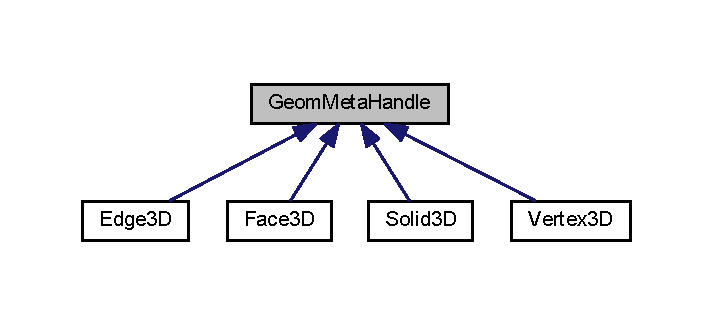
\includegraphics[width=342pt]{class_geom_meta_handle__inherit__graph}
\end{center}
\end{figure}
\subsection*{Public Member Functions}
\begin{DoxyCompactItemize}
\item 
\hypertarget{class_geom_meta_handle_a1787f612c3a943eda6368722713681f9}{\hyperlink{class_geom_meta_handle_a1787f612c3a943eda6368722713681f9}{Geom\-Meta\-Handle} ()}\label{class_geom_meta_handle_a1787f612c3a943eda6368722713681f9}

\begin{DoxyCompactList}\small\item\em Default constructor. Initialises values to null. \end{DoxyCompactList}\end{DoxyCompactItemize}
\subsection*{Public Attributes}
\begin{DoxyCompactItemize}
\item 
bool \hyperlink{class_geom_meta_handle_a545e915bdbffcafcf5cd9381b404874c}{m\-\_\-b\-Selected}
\end{DoxyCompactItemize}


\subsection{Detailed Description}
Metaclass which all geometry components subclass from. Contains useful metadata relevant to geometry components. 

\subsection{Member Data Documentation}
\hypertarget{class_geom_meta_handle_a545e915bdbffcafcf5cd9381b404874c}{\index{Geom\-Meta\-Handle@{Geom\-Meta\-Handle}!m\-\_\-b\-Selected@{m\-\_\-b\-Selected}}
\index{m\-\_\-b\-Selected@{m\-\_\-b\-Selected}!GeomMetaHandle@{Geom\-Meta\-Handle}}
\subsubsection[{m\-\_\-b\-Selected}]{\setlength{\rightskip}{0pt plus 5cm}bool Geom\-Meta\-Handle\-::m\-\_\-b\-Selected}}\label{class_geom_meta_handle_a545e915bdbffcafcf5cd9381b404874c}
Whether the component is currently selected. 

The documentation for this class was generated from the following file\-:\begin{DoxyCompactItemize}
\item 
app/\hyperlink{vertex_8h}{vertex.\-h}\end{DoxyCompactItemize}

\hypertarget{class_i_command_box}{\section{I\-Command\-Box Class Reference}
\label{class_i_command_box}\index{I\-Command\-Box@{I\-Command\-Box}}
}
\subsection*{Public Member Functions}
\begin{DoxyCompactItemize}
\item 
\hypertarget{class_i_command_box_a2f6e39cddc355cf526e98a2b2884352b}{virtual void {\bfseries show\-Suggestions} (const Q\-String\-List \&list)=0}\label{class_i_command_box_a2f6e39cddc355cf526e98a2b2884352b}

\end{DoxyCompactItemize}


The documentation for this class was generated from the following file\-:\begin{DoxyCompactItemize}
\item 
I\-Console/interfaces/\hyperlink{icommandbox_8h}{icommandbox.\-h}\end{DoxyCompactItemize}

\hypertarget{class_i_command_manager}{\section{I\-Command\-Manager Class Reference}
\label{class_i_command_manager}\index{I\-Command\-Manager@{I\-Command\-Manager}}
}
\subsection*{Public Types}
\begin{DoxyCompactItemize}
\item 
\hypertarget{class_i_command_manager_aad93f45962c23c66dbb643b2a437a6b5}{typedef int($\ast$ {\bfseries Cmd\-Callback} )(const Q\-String \&, const Q\-String\-List \&)}\label{class_i_command_manager_aad93f45962c23c66dbb643b2a437a6b5}

\item 
\hypertarget{class_i_command_manager_a8ca7fae732c3682aa0d0120b81570eb4}{typedef void($\ast$ {\bfseries Var\-Callback} )(const Q\-String \&, Q\-String \&)}\label{class_i_command_manager_a8ca7fae732c3682aa0d0120b81570eb4}

\end{DoxyCompactItemize}
\subsection*{Public Member Functions}
\begin{DoxyCompactItemize}
\item 
\hypertarget{class_i_command_manager_a04ad1ccf7336d550c9bb46d38417196c}{virtual bool {\bfseries register\-Command} (Q\-String \&name, Cmd\-Callback callback, Q\-String \&description=\char`\"{}\char`\"{}, unsigned int flags=0)=0}\label{class_i_command_manager_a04ad1ccf7336d550c9bb46d38417196c}

\item 
\hypertarget{class_i_command_manager_af2642fcd4711e203d6caadc48e147492}{virtual bool {\bfseries register\-Variable} (Q\-String \&name, Var\-Callback callback=N\-U\-L\-L, Q\-String \&description=\char`\"{}\char`\"{}, unsigned int flags=0, bool has\-Min=false, float min=0.\-0, bool has\-Max=false, float max=0.\-0)=0}\label{class_i_command_manager_af2642fcd4711e203d6caadc48e147492}

\item 
\hypertarget{class_i_command_manager_a8ea6c917b51e564a937ded9ac40cd265}{virtual void {\bfseries unregister} (Q\-String \&name)=0}\label{class_i_command_manager_a8ea6c917b51e564a937ded9ac40cd265}

\item 
\hypertarget{class_i_command_manager_a6f32752cbd34de65d4194fabd3d4ff22}{virtual int {\bfseries exec} (Q\-String \&name, Q\-Variant $\ast$const variable=N\-U\-L\-L)=0}\label{class_i_command_manager_a6f32752cbd34de65d4194fabd3d4ff22}

\item 
\hypertarget{class_i_command_manager_a883397692f50a33c1442ad743b599b9a}{virtual void {\bfseries suggest} (const Q\-String \&partial\-Cmd, Q\-String\-List \&suggestions)=0}\label{class_i_command_manager_a883397692f50a33c1442ad743b599b9a}

\end{DoxyCompactItemize}


The documentation for this class was generated from the following file\-:\begin{DoxyCompactItemize}
\item 
I\-Console/interfaces/\hyperlink{icommandmanager_8h}{icommandmanager.\-h}\end{DoxyCompactItemize}

\hypertarget{class_i_completion_widget}{\section{I\-Completion\-Widget Class Reference}
\label{class_i_completion_widget}\index{I\-Completion\-Widget@{I\-Completion\-Widget}}
}
\subsection*{Public Member Functions}
\begin{DoxyCompactItemize}
\item 
\hypertarget{class_i_completion_widget_a7d4605c0db4a8181d4ab106f3f073210}{virtual void {\bfseries show\-List} (Q\-String\-List \&list)=0}\label{class_i_completion_widget_a7d4605c0db4a8181d4ab106f3f073210}

\item 
\hypertarget{class_i_completion_widget_a2d3553dd808ca776848720e454711a63}{virtual Q\-String {\bfseries get\-Highlighted} () const =0}\label{class_i_completion_widget_a2d3553dd808ca776848720e454711a63}

\item 
\hypertarget{class_i_completion_widget_a6f42b642287323cd4affdfd99ae9fa41}{virtual void {\bfseries increment\-Highlight} ()=0}\label{class_i_completion_widget_a6f42b642287323cd4affdfd99ae9fa41}

\end{DoxyCompactItemize}


The documentation for this class was generated from the following file\-:\begin{DoxyCompactItemize}
\item 
I\-Console/interfaces/icompletionwidget.\-h\end{DoxyCompactItemize}

\hypertarget{class_i_console_window}{\section{I\-Console\-Window Class Reference}
\label{class_i_console_window}\index{I\-Console\-Window@{I\-Console\-Window}}
}


Inheritance diagram for I\-Console\-Window\-:
\nopagebreak
\begin{figure}[H]
\begin{center}
\leavevmode
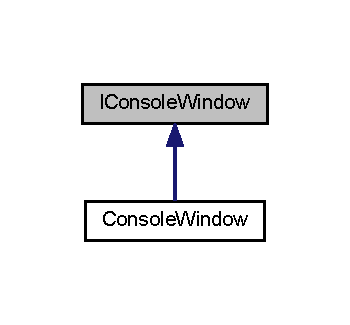
\includegraphics[width=168pt]{class_i_console_window__inherit__graph}
\end{center}
\end{figure}
\subsection*{Public Member Functions}
\begin{DoxyCompactItemize}
\item 
\hypertarget{class_i_console_window_a7fe4cfa09149ac529a44aa87d7d813b3}{virtual void {\bfseries print\-Message} (const Q\-String \&message)=0}\label{class_i_console_window_a7fe4cfa09149ac529a44aa87d7d813b3}

\item 
\hypertarget{class_i_console_window_a64f0fac283cd4f584e6ecc6e4b97fcbd}{virtual void {\bfseries print\-Warning} (const Q\-String \&message)=0}\label{class_i_console_window_a64f0fac283cd4f584e6ecc6e4b97fcbd}

\end{DoxyCompactItemize}


The documentation for this class was generated from the following file\-:\begin{DoxyCompactItemize}
\item 
I\-Console/interfaces/\hyperlink{iconsolewindow_8h}{iconsolewindow.\-h}\end{DoxyCompactItemize}

\hypertarget{class_index_pool}{\section{Index\-Pool Class Reference}
\label{class_index_pool}\index{Index\-Pool@{Index\-Pool}}
}


The \hyperlink{class_index_pool}{Index\-Pool} class manages non-\/consecutive array indices.  




{\ttfamily \#include $<$indexpool.\-h$>$}



Inheritance diagram for Index\-Pool\-:\nopagebreak
\begin{figure}[H]
\begin{center}
\leavevmode
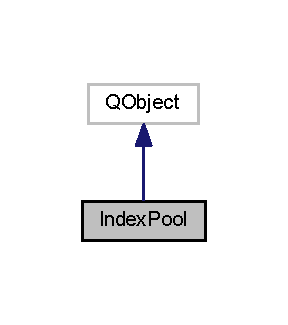
\includegraphics[width=138pt]{class_index_pool__inherit__graph}
\end{center}
\end{figure}


Collaboration diagram for Index\-Pool\-:\nopagebreak
\begin{figure}[H]
\begin{center}
\leavevmode
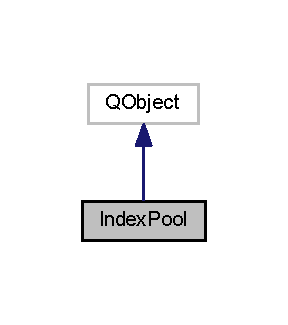
\includegraphics[width=138pt]{class_index_pool__coll__graph}
\end{center}
\end{figure}
\subsection*{Public Types}
\begin{DoxyCompactItemize}
\item 
enum \{ \hyperlink{class_index_pool_abacc88fb0ea6d1dcad5be70710ed0e3da3a3d6446453050cd4c95439b37b6824a}{I\-N\-D\-E\-X\-\_\-\-L\-I\-M\-I\-T} = 4294967294
 \}
\end{DoxyCompactItemize}
\subsection*{Public Slots}
\begin{DoxyCompactItemize}
\item 
void \hyperlink{class_index_pool_a7791b409b32242230867480c9b79de15}{release\-Index} (const \hyperlink{vertex_8h_a72202e57358ed73cd212e9a2eaf39aeb}{G\-E\-O\-M\-H\-A\-N\-D\-L\-E} index)
\begin{DoxyCompactList}\small\item\em Releases an index, allowing it to be allocated again. \end{DoxyCompactList}\item 
\hypertarget{class_index_pool_abda4a4fa05598f52c3af955788904c9f}{void \hyperlink{class_index_pool_abda4a4fa05598f52c3af955788904c9f}{condense} ()}\label{class_index_pool_abda4a4fa05598f52c3af955788904c9f}

\begin{DoxyCompactList}\small\item\em Condenses all indices (shifts indices down to fill all \char`\"{}holes\char`\"{} in the array). index\-Reallocation is fired for each re-\/allocated index. \end{DoxyCompactList}\end{DoxyCompactItemize}
\subsection*{Signals}
\begin{DoxyCompactItemize}
\item 
void \hyperlink{class_index_pool_a80b1499f90029a3531fc0603a5420cd8}{index\-Reallocation} (\hyperlink{vertex_8h_a72202e57358ed73cd212e9a2eaf39aeb}{G\-E\-O\-M\-H\-A\-N\-D\-L\-E} old\-Value, \hyperlink{vertex_8h_a72202e57358ed73cd212e9a2eaf39aeb}{G\-E\-O\-M\-H\-A\-N\-D\-L\-E} new\-Value)
\begin{DoxyCompactList}\small\item\em Fired when indices are re-\/allocated by \hyperlink{class_index_pool_abda4a4fa05598f52c3af955788904c9f}{condense()}. Any indices whose value does not get passed through this signal as old\-Value remains at its original value. \end{DoxyCompactList}\end{DoxyCompactItemize}
\subsection*{Public Member Functions}
\begin{DoxyCompactItemize}
\item 
\hyperlink{class_index_pool_a26e3c07764def73d6ebf8a1df0ce9bb4}{Index\-Pool} (Q\-Object $\ast$parent=0, \hyperlink{vertex_8h_a72202e57358ed73cd212e9a2eaf39aeb}{G\-E\-O\-M\-H\-A\-N\-D\-L\-E} highest\-Index=\hyperlink{class_index_pool_abacc88fb0ea6d1dcad5be70710ed0e3da3a3d6446453050cd4c95439b37b6824a}{I\-N\-D\-E\-X\-\_\-\-L\-I\-M\-I\-T})
\begin{DoxyCompactList}\small\item\em Constructor. \end{DoxyCompactList}\item 
bool \hyperlink{class_index_pool_a6001551942dde955048c7fdca82cbda7}{is\-Allocated} (\hyperlink{vertex_8h_a72202e57358ed73cd212e9a2eaf39aeb}{G\-E\-O\-M\-H\-A\-N\-D\-L\-E} index) const 
\begin{DoxyCompactList}\small\item\em Returns whether the specified index is currently allocated. \end{DoxyCompactList}\item 
bool \hyperlink{class_index_pool_a6f3dade75f8853215eb40b8dc9593f6c}{get\-Highest\-Allowed\-Index} () const 
\begin{DoxyCompactList}\small\item\em Returns the maximum index which can be allocated by this pool. \end{DoxyCompactList}\item 
\hyperlink{vertex_8h_a72202e57358ed73cd212e9a2eaf39aeb}{G\-E\-O\-M\-H\-A\-N\-D\-L\-E} \hyperlink{class_index_pool_a47301791c0015a14e7f459ae3efb614c}{allocate\-Index} ()
\begin{DoxyCompactList}\small\item\em Allocates the lowest free index. \end{DoxyCompactList}\end{DoxyCompactItemize}


\subsection{Detailed Description}
The \hyperlink{class_index_pool}{Index\-Pool} class manages non-\/consecutive array indices. 

The index pool works on the following heuristics\-:\par
 
\begin{DoxyItemize}
\item If the current number of allocated indices is contiguous (or nothing), the new index is allocated at the end of the current block of indices. 
\item If the current number of allocated indices is non-\/contiguous, the lowest unused index is allocated.
\end{DoxyItemize}\par
 This means that when indices are deallocated, \char`\"{}holes\char`\"{} in the array of indices are filled first before new indices are added to the end of the array. 

\subsection{Member Enumeration Documentation}
\hypertarget{class_index_pool_abacc88fb0ea6d1dcad5be70710ed0e3d}{\subsubsection[{anonymous enum}]{\setlength{\rightskip}{0pt plus 5cm}anonymous enum}}\label{class_index_pool_abacc88fb0ea6d1dcad5be70710ed0e3d}
\begin{Desc}
\item[Enumerator]\par
\begin{description}
\index{I\-N\-D\-E\-X\-\_\-\-L\-I\-M\-I\-T@{I\-N\-D\-E\-X\-\_\-\-L\-I\-M\-I\-T}!Index\-Pool@{Index\-Pool}}\index{Index\-Pool@{Index\-Pool}!I\-N\-D\-E\-X\-\_\-\-L\-I\-M\-I\-T@{I\-N\-D\-E\-X\-\_\-\-L\-I\-M\-I\-T}}\item[{\em 
\hypertarget{class_index_pool_abacc88fb0ea6d1dcad5be70710ed0e3da3a3d6446453050cd4c95439b37b6824a}{I\-N\-D\-E\-X\-\_\-\-L\-I\-M\-I\-T}\label{class_index_pool_abacc88fb0ea6d1dcad5be70710ed0e3da3a3d6446453050cd4c95439b37b6824a}
}]Highest allocatable index. \end{description}
\end{Desc}


\subsection{Constructor \& Destructor Documentation}
\hypertarget{class_index_pool_a26e3c07764def73d6ebf8a1df0ce9bb4}{\index{Index\-Pool@{Index\-Pool}!Index\-Pool@{Index\-Pool}}
\index{Index\-Pool@{Index\-Pool}!IndexPool@{Index\-Pool}}
\subsubsection[{Index\-Pool}]{\setlength{\rightskip}{0pt plus 5cm}Index\-Pool\-::\-Index\-Pool (
\begin{DoxyParamCaption}
\item[{Q\-Object $\ast$}]{parent = {\ttfamily 0}, }
\item[{{\bf G\-E\-O\-M\-H\-A\-N\-D\-L\-E}}]{highest\-Index = {\ttfamily {\bf I\-N\-D\-E\-X\-\_\-\-L\-I\-M\-I\-T}}}
\end{DoxyParamCaption}
)\hspace{0.3cm}{\ttfamily [explicit]}}}\label{class_index_pool_a26e3c07764def73d6ebf8a1df0ce9bb4}


Constructor. 


\begin{DoxyParams}{Parameters}
{\em parent} & Parent object. \\
\hline
{\em highest\-Index} & Highest number of indices. \\
\hline
\end{DoxyParams}


\subsection{Member Function Documentation}
\hypertarget{class_index_pool_a47301791c0015a14e7f459ae3efb614c}{\index{Index\-Pool@{Index\-Pool}!allocate\-Index@{allocate\-Index}}
\index{allocate\-Index@{allocate\-Index}!IndexPool@{Index\-Pool}}
\subsubsection[{allocate\-Index}]{\setlength{\rightskip}{0pt plus 5cm}{\bf G\-E\-O\-M\-H\-A\-N\-D\-L\-E} Index\-Pool\-::allocate\-Index (
\begin{DoxyParamCaption}
{}
\end{DoxyParamCaption}
)}}\label{class_index_pool_a47301791c0015a14e7f459ae3efb614c}


Allocates the lowest free index. 

\begin{DoxyReturn}{Returns}
Allocated index, or N\-U\-L\-L\-H\-N\-D if no more indices could be allocated. 
\end{DoxyReturn}
\hypertarget{class_index_pool_a6f3dade75f8853215eb40b8dc9593f6c}{\index{Index\-Pool@{Index\-Pool}!get\-Highest\-Allowed\-Index@{get\-Highest\-Allowed\-Index}}
\index{get\-Highest\-Allowed\-Index@{get\-Highest\-Allowed\-Index}!IndexPool@{Index\-Pool}}
\subsubsection[{get\-Highest\-Allowed\-Index}]{\setlength{\rightskip}{0pt plus 5cm}bool Index\-Pool\-::get\-Highest\-Allowed\-Index (
\begin{DoxyParamCaption}
{}
\end{DoxyParamCaption}
) const\hspace{0.3cm}{\ttfamily [inline]}}}\label{class_index_pool_a6f3dade75f8853215eb40b8dc9593f6c}


Returns the maximum index which can be allocated by this pool. 

\begin{DoxyReturn}{Returns}
Highest allowed index. 
\end{DoxyReturn}
\hypertarget{class_index_pool_a80b1499f90029a3531fc0603a5420cd8}{\index{Index\-Pool@{Index\-Pool}!index\-Reallocation@{index\-Reallocation}}
\index{index\-Reallocation@{index\-Reallocation}!IndexPool@{Index\-Pool}}
\subsubsection[{index\-Reallocation}]{\setlength{\rightskip}{0pt plus 5cm}void Index\-Pool\-::index\-Reallocation (
\begin{DoxyParamCaption}
\item[{{\bf G\-E\-O\-M\-H\-A\-N\-D\-L\-E}}]{old\-Value, }
\item[{{\bf G\-E\-O\-M\-H\-A\-N\-D\-L\-E}}]{new\-Value}
\end{DoxyParamCaption}
)\hspace{0.3cm}{\ttfamily [signal]}}}\label{class_index_pool_a80b1499f90029a3531fc0603a5420cd8}


Fired when indices are re-\/allocated by \hyperlink{class_index_pool_abda4a4fa05598f52c3af955788904c9f}{condense()}. Any indices whose value does not get passed through this signal as old\-Value remains at its original value. 


\begin{DoxyParams}{Parameters}
{\em old\-Value} & Old value of index. \\
\hline
{\em new\-Value} & The index's new value. \\
\hline
\end{DoxyParams}
\hypertarget{class_index_pool_a6001551942dde955048c7fdca82cbda7}{\index{Index\-Pool@{Index\-Pool}!is\-Allocated@{is\-Allocated}}
\index{is\-Allocated@{is\-Allocated}!IndexPool@{Index\-Pool}}
\subsubsection[{is\-Allocated}]{\setlength{\rightskip}{0pt plus 5cm}bool Index\-Pool\-::is\-Allocated (
\begin{DoxyParamCaption}
\item[{{\bf G\-E\-O\-M\-H\-A\-N\-D\-L\-E}}]{index}
\end{DoxyParamCaption}
) const}}\label{class_index_pool_a6001551942dde955048c7fdca82cbda7}


Returns whether the specified index is currently allocated. 


\begin{DoxyParams}{Parameters}
{\em index} & Index to check. \\
\hline
\end{DoxyParams}
\begin{DoxyReturn}{Returns}
True if already allocated, false if not. 
\end{DoxyReturn}
\hypertarget{class_index_pool_a7791b409b32242230867480c9b79de15}{\index{Index\-Pool@{Index\-Pool}!release\-Index@{release\-Index}}
\index{release\-Index@{release\-Index}!IndexPool@{Index\-Pool}}
\subsubsection[{release\-Index}]{\setlength{\rightskip}{0pt plus 5cm}void Index\-Pool\-::release\-Index (
\begin{DoxyParamCaption}
\item[{const {\bf G\-E\-O\-M\-H\-A\-N\-D\-L\-E}}]{index}
\end{DoxyParamCaption}
)\hspace{0.3cm}{\ttfamily [slot]}}}\label{class_index_pool_a7791b409b32242230867480c9b79de15}


Releases an index, allowing it to be allocated again. 


\begin{DoxyParams}{Parameters}
{\em index} & Index to release. \\
\hline
\end{DoxyParams}


The documentation for this class was generated from the following files\-:\begin{DoxyCompactItemize}
\item 
app/\hyperlink{indexpool_8h}{indexpool.\-h}\item 
app/indexpool.\-cpp\end{DoxyCompactItemize}

\hypertarget{class_i_plugin}{\section{I\-Plugin Class Reference}
\label{class_i_plugin}\index{I\-Plugin@{I\-Plugin}}
}


Required core interface for a Crowbar plugin.  




{\ttfamily \#include $<$plugin.\-h$>$}

\subsection*{Public Member Functions}
\begin{DoxyCompactItemize}
\item 
virtual Q\-String \hyperlink{class_i_plugin_a8c0c4c970a8b59c8c7f66e1fec3045a3}{Get\-Unique\-Id} ()=0
\begin{DoxyCompactList}\small\item\em Returns the plugin's unique I\-D string. \end{DoxyCompactList}\item 
virtual Q\-String \hyperlink{class_i_plugin_a5f07a9a06d9abb95156ea70818c63386}{Get\-Author} ()=0
\begin{DoxyCompactList}\small\item\em Returns the plugin's author. \end{DoxyCompactList}\item 
virtual void \hyperlink{class_i_plugin_ae274cc3ddc9ccd4c7ee22a4da1cc2d94}{Get\-Version} (\hyperlink{plugin_8h_a725de6c68b62463ee6792bb48710febe}{Plugin\-Version} $\ast$version)=0
\begin{DoxyCompactList}\small\item\em Modifies the passed Plugin\-Version array to return this plugin's version. \end{DoxyCompactList}\end{DoxyCompactItemize}


\subsection{Detailed Description}
Required core interface for a Crowbar plugin. 

\subsection{Member Function Documentation}
\hypertarget{class_i_plugin_a5f07a9a06d9abb95156ea70818c63386}{\index{I\-Plugin@{I\-Plugin}!Get\-Author@{Get\-Author}}
\index{Get\-Author@{Get\-Author}!IPlugin@{I\-Plugin}}
\subsubsection[{Get\-Author}]{\setlength{\rightskip}{0pt plus 5cm}virtual Q\-String I\-Plugin\-::\-Get\-Author (
\begin{DoxyParamCaption}
{}
\end{DoxyParamCaption}
)\hspace{0.3cm}{\ttfamily [pure virtual]}}}\label{class_i_plugin_a5f07a9a06d9abb95156ea70818c63386}


Returns the plugin's author. 

\begin{DoxyReturn}{Returns}
Plugin's author. 
\end{DoxyReturn}
\hypertarget{class_i_plugin_a8c0c4c970a8b59c8c7f66e1fec3045a3}{\index{I\-Plugin@{I\-Plugin}!Get\-Unique\-Id@{Get\-Unique\-Id}}
\index{Get\-Unique\-Id@{Get\-Unique\-Id}!IPlugin@{I\-Plugin}}
\subsubsection[{Get\-Unique\-Id}]{\setlength{\rightskip}{0pt plus 5cm}virtual Q\-String I\-Plugin\-::\-Get\-Unique\-Id (
\begin{DoxyParamCaption}
{}
\end{DoxyParamCaption}
)\hspace{0.3cm}{\ttfamily [pure virtual]}}}\label{class_i_plugin_a8c0c4c970a8b59c8c7f66e1fec3045a3}


Returns the plugin's unique I\-D string. 

\begin{DoxyNote}{Note}
If a loaded plugin with an I\-D string already exists, subsequent plugins with this I\-D will fail to load. 
\end{DoxyNote}
\begin{DoxyReturn}{Returns}
I\-D string. 
\end{DoxyReturn}
\hypertarget{class_i_plugin_ae274cc3ddc9ccd4c7ee22a4da1cc2d94}{\index{I\-Plugin@{I\-Plugin}!Get\-Version@{Get\-Version}}
\index{Get\-Version@{Get\-Version}!IPlugin@{I\-Plugin}}
\subsubsection[{Get\-Version}]{\setlength{\rightskip}{0pt plus 5cm}virtual void I\-Plugin\-::\-Get\-Version (
\begin{DoxyParamCaption}
\item[{{\bf Plugin\-Version} $\ast$}]{version}
\end{DoxyParamCaption}
)\hspace{0.3cm}{\ttfamily [pure virtual]}}}\label{class_i_plugin_ae274cc3ddc9ccd4c7ee22a4da1cc2d94}


Modifies the passed Plugin\-Version array to return this plugin's version. 


\begin{DoxyParams}{Parameters}
{\em version} & Array to hold the plugin's version. \\
\hline
\end{DoxyParams}


The documentation for this class was generated from the following file\-:\begin{DoxyCompactItemize}
\item 
app/\hyperlink{plugin_8h}{plugin.\-h}\end{DoxyCompactItemize}

\hypertarget{class_i_vertex3_d_render_spec}{\section{I\-Vertex3\-D\-Render\-Spec Class Reference}
\label{class_i_vertex3_d_render_spec}\index{I\-Vertex3\-D\-Render\-Spec@{I\-Vertex3\-D\-Render\-Spec}}
}


Defines the properties required to be exposed by renderable vertices.  




{\ttfamily \#include $<$ivertex3drenderspec.\-h$>$}



Inheritance diagram for I\-Vertex3\-D\-Render\-Spec\-:
\nopagebreak
\begin{figure}[H]
\begin{center}
\leavevmode
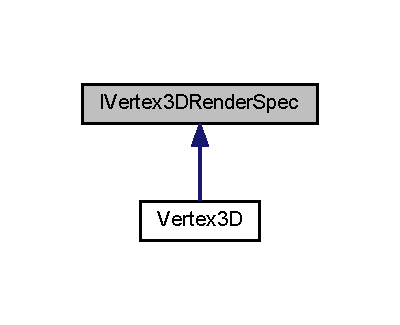
\includegraphics[width=192pt]{class_i_vertex3_d_render_spec__inherit__graph}
\end{center}
\end{figure}
\subsection*{Public Types}
\begin{DoxyCompactItemize}
\item 
enum \{ {\bfseries V3\-R\-S\-\_\-\-T\-O\-T\-A\-L\-\_\-\-D\-A\-T\-A\-\_\-\-T\-R\-A\-N\-S\-F\-E\-R} = 24
 \}
\end{DoxyCompactItemize}
\subsection*{Public Member Functions}
\begin{DoxyCompactItemize}
\item 
virtual unsigned long \hyperlink{class_i_vertex3_d_render_spec_a891d736d3d414de333398975f34bbae7}{V3\-R\-S\-\_\-\-Offset} ()=0
\begin{DoxyCompactList}\small\item\em Returns the offset of this vertex from the beginning of the V\-B\-O, in V3\-R\-S\-\_\-\-T\-O\-T\-A\-L\-\_\-\-D\-A\-T\-A\-\_\-\-T\-R\-A\-N\-S\-F\-E\-R steps. \end{DoxyCompactList}\item 
virtual void \hyperlink{class_i_vertex3_d_render_spec_a198bcfd0e8b6996848da0babe6805213}{V3\-R\-S\-\_\-\-Position} (float position\mbox{[}3\mbox{]})=0
\begin{DoxyCompactList}\small\item\em Fills an array with the position values for this vertex. \end{DoxyCompactList}\item 
virtual void \hyperlink{class_i_vertex3_d_render_spec_aaa32fb05761effc71596ee25c0eaaa77}{V3\-R\-S\-\_\-\-Colour} (unsigned char colour\mbox{[}4\mbox{]})=0
\begin{DoxyCompactList}\small\item\em Fills an array with the colour values for this vertex. \end{DoxyCompactList}\item 
virtual void \hyperlink{class_i_vertex3_d_render_spec_af9b255329a6ea9dd75e18699792b03e8}{V3\-R\-S\-\_\-\-Texture\-\_\-\-Coords} (float coords\mbox{[}2\mbox{]})=0
\begin{DoxyCompactList}\small\item\em Fills an array with the texture co-\/ordinate values for this vertex. \end{DoxyCompactList}\end{DoxyCompactItemize}


\subsection{Detailed Description}
Defines the properties required to be exposed by renderable vertices. 

\subsection{Member Function Documentation}
\hypertarget{class_i_vertex3_d_render_spec_aaa32fb05761effc71596ee25c0eaaa77}{\index{I\-Vertex3\-D\-Render\-Spec@{I\-Vertex3\-D\-Render\-Spec}!V3\-R\-S\-\_\-\-Colour@{V3\-R\-S\-\_\-\-Colour}}
\index{V3\-R\-S\-\_\-\-Colour@{V3\-R\-S\-\_\-\-Colour}!IVertex3DRenderSpec@{I\-Vertex3\-D\-Render\-Spec}}
\subsubsection[{V3\-R\-S\-\_\-\-Colour}]{\setlength{\rightskip}{0pt plus 5cm}virtual void I\-Vertex3\-D\-Render\-Spec\-::\-V3\-R\-S\-\_\-\-Colour (
\begin{DoxyParamCaption}
\item[{unsigned char}]{colour\mbox{[}4\mbox{]}}
\end{DoxyParamCaption}
)\hspace{0.3cm}{\ttfamily [pure virtual]}}}\label{class_i_vertex3_d_render_spec_aaa32fb05761effc71596ee25c0eaaa77}


Fills an array with the colour values for this vertex. 


\begin{DoxyParams}{Parameters}
{\em colour} & Colour values. Format is R\-G\-B\-A, range 0-\/255. \\
\hline
\end{DoxyParams}
\hypertarget{class_i_vertex3_d_render_spec_a891d736d3d414de333398975f34bbae7}{\index{I\-Vertex3\-D\-Render\-Spec@{I\-Vertex3\-D\-Render\-Spec}!V3\-R\-S\-\_\-\-Offset@{V3\-R\-S\-\_\-\-Offset}}
\index{V3\-R\-S\-\_\-\-Offset@{V3\-R\-S\-\_\-\-Offset}!IVertex3DRenderSpec@{I\-Vertex3\-D\-Render\-Spec}}
\subsubsection[{V3\-R\-S\-\_\-\-Offset}]{\setlength{\rightskip}{0pt plus 5cm}virtual unsigned long I\-Vertex3\-D\-Render\-Spec\-::\-V3\-R\-S\-\_\-\-Offset (
\begin{DoxyParamCaption}
{}
\end{DoxyParamCaption}
)\hspace{0.3cm}{\ttfamily [pure virtual]}}}\label{class_i_vertex3_d_render_spec_a891d736d3d414de333398975f34bbae7}


Returns the offset of this vertex from the beginning of the V\-B\-O, in V3\-R\-S\-\_\-\-T\-O\-T\-A\-L\-\_\-\-D\-A\-T\-A\-\_\-\-T\-R\-A\-N\-S\-F\-E\-R steps. 

\begin{DoxyReturn}{Returns}
Offset for this vertex. 
\end{DoxyReturn}


Implemented in \hyperlink{class_vertex3_d_a13a922fd8180591636c1daf4687cc205}{Vertex3\-D}.

\hypertarget{class_i_vertex3_d_render_spec_a198bcfd0e8b6996848da0babe6805213}{\index{I\-Vertex3\-D\-Render\-Spec@{I\-Vertex3\-D\-Render\-Spec}!V3\-R\-S\-\_\-\-Position@{V3\-R\-S\-\_\-\-Position}}
\index{V3\-R\-S\-\_\-\-Position@{V3\-R\-S\-\_\-\-Position}!IVertex3DRenderSpec@{I\-Vertex3\-D\-Render\-Spec}}
\subsubsection[{V3\-R\-S\-\_\-\-Position}]{\setlength{\rightskip}{0pt plus 5cm}virtual void I\-Vertex3\-D\-Render\-Spec\-::\-V3\-R\-S\-\_\-\-Position (
\begin{DoxyParamCaption}
\item[{float}]{position\mbox{[}3\mbox{]}}
\end{DoxyParamCaption}
)\hspace{0.3cm}{\ttfamily [pure virtual]}}}\label{class_i_vertex3_d_render_spec_a198bcfd0e8b6996848da0babe6805213}


Fills an array with the position values for this vertex. 


\begin{DoxyParams}{Parameters}
{\em position} & Array to fill. Format is X\-Y\-Z. \\
\hline
\end{DoxyParams}
\hypertarget{class_i_vertex3_d_render_spec_af9b255329a6ea9dd75e18699792b03e8}{\index{I\-Vertex3\-D\-Render\-Spec@{I\-Vertex3\-D\-Render\-Spec}!V3\-R\-S\-\_\-\-Texture\-\_\-\-Coords@{V3\-R\-S\-\_\-\-Texture\-\_\-\-Coords}}
\index{V3\-R\-S\-\_\-\-Texture\-\_\-\-Coords@{V3\-R\-S\-\_\-\-Texture\-\_\-\-Coords}!IVertex3DRenderSpec@{I\-Vertex3\-D\-Render\-Spec}}
\subsubsection[{V3\-R\-S\-\_\-\-Texture\-\_\-\-Coords}]{\setlength{\rightskip}{0pt plus 5cm}virtual void I\-Vertex3\-D\-Render\-Spec\-::\-V3\-R\-S\-\_\-\-Texture\-\_\-\-Coords (
\begin{DoxyParamCaption}
\item[{float}]{coords\mbox{[}2\mbox{]}}
\end{DoxyParamCaption}
)\hspace{0.3cm}{\ttfamily [pure virtual]}}}\label{class_i_vertex3_d_render_spec_af9b255329a6ea9dd75e18699792b03e8}


Fills an array with the texture co-\/ordinate values for this vertex. 


\begin{DoxyParams}{Parameters}
{\em coords} & Array to fill. Format is X\-Y. \\
\hline
\end{DoxyParams}


The documentation for this class was generated from the following file\-:\begin{DoxyCompactItemize}
\item 
app/\hyperlink{ivertex3drenderspec_8h}{ivertex3drenderspec.\-h}\end{DoxyCompactItemize}

\hypertarget{class_log_window}{\section{Log\-Window Class Reference}
\label{class_log_window}\index{Log\-Window@{Log\-Window}}
}


Logging window.  




{\ttfamily \#include $<$logwindow.\-h$>$}



Inheritance diagram for Log\-Window\-:
\nopagebreak
\begin{figure}[H]
\begin{center}
\leavevmode
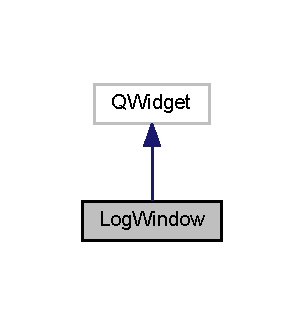
\includegraphics[width=146pt]{class_log_window__inherit__graph}
\end{center}
\end{figure}


Collaboration diagram for Log\-Window\-:
\nopagebreak
\begin{figure}[H]
\begin{center}
\leavevmode
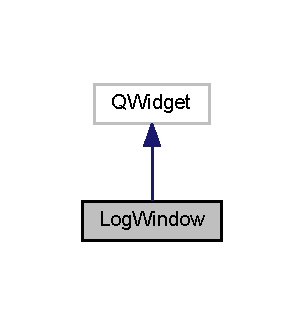
\includegraphics[width=146pt]{class_log_window__coll__graph}
\end{center}
\end{figure}
\subsection*{Public Slots}
\begin{DoxyCompactItemize}
\item 
\hypertarget{class_log_window_adcc6e0cdf92339342b6d564969c9c08a}{void \hyperlink{class_log_window_adcc6e0cdf92339342b6d564969c9c08a}{show} ()}\label{class_log_window_adcc6e0cdf92339342b6d564969c9c08a}

\begin{DoxyCompactList}\small\item\em Shows the logging window. \end{DoxyCompactList}\item 
\hypertarget{class_log_window_a0e2b0c1b3532f71fbff15d038417f108}{void \hyperlink{class_log_window_a0e2b0c1b3532f71fbff15d038417f108}{show\-And\-Raise} ()}\label{class_log_window_a0e2b0c1b3532f71fbff15d038417f108}

\begin{DoxyCompactList}\small\item\em Shows the logging window and raises it to be on top of any other windows. \end{DoxyCompactList}\item 
void \hyperlink{class_log_window_ac001882d402237088e250734cd98838c}{print\-Message} (Q\-String message)
\begin{DoxyCompactList}\small\item\em Prints a message to the log window (but not to a log file). \end{DoxyCompactList}\item 
void \hyperlink{class_log_window_ad22aacde45b6bbb323a7f2a4d8aba94b}{log\-Message} (Q\-String message)
\begin{DoxyCompactList}\small\item\em Writes a message to a log file (but does not print to the log window). \end{DoxyCompactList}\item 
void \hyperlink{class_log_window_a6e465543f32c1b9447ccbb481eee9407}{print\-Warning} (Q\-String message)
\begin{DoxyCompactList}\small\item\em Prints a warning to the log window (but not to a log file). \end{DoxyCompactList}\item 
void \hyperlink{class_log_window_adde69360b38aad4e23ee16100adba710}{log\-Warning} (Q\-String message)
\begin{DoxyCompactList}\small\item\em Writes a warning to a log file (but does not print to the log window). \end{DoxyCompactList}\item 
\hypertarget{class_log_window_af2db9c420af21e1c07b416a6a3a7e5a2}{void \hyperlink{class_log_window_af2db9c420af21e1c07b416a6a3a7e5a2}{zoom\-In} ()}\label{class_log_window_af2db9c420af21e1c07b416a6a3a7e5a2}

\begin{DoxyCompactList}\small\item\em Makes the log window text larger. \end{DoxyCompactList}\item 
\hypertarget{class_log_window_ae534c7a6486b7223427dc2ad65316b09}{void \hyperlink{class_log_window_ae534c7a6486b7223427dc2ad65316b09}{zoom\-Out} ()}\label{class_log_window_ae534c7a6486b7223427dc2ad65316b09}

\begin{DoxyCompactList}\small\item\em Makes the log window text smaller. \end{DoxyCompactList}\item 
\hypertarget{class_log_window_a18658a91b3a65b744a684994ab247dde}{void \hyperlink{class_log_window_a18658a91b3a65b744a684994ab247dde}{new\-Log\-File} ()}\label{class_log_window_a18658a91b3a65b744a684994ab247dde}

\begin{DoxyCompactList}\small\item\em Creates a new log file whose name is based on the current date and time. \end{DoxyCompactList}\item 
void \hyperlink{class_log_window_a903fc2156c1aa3f72c28fff20ecee6e3}{new\-Log\-File} (Q\-String filename)
\begin{DoxyCompactList}\small\item\em Creates a new log file. \end{DoxyCompactList}\end{DoxyCompactItemize}
\subsection*{Public Member Functions}
\begin{DoxyCompactItemize}
\item 
\hyperlink{class_log_window_a3c1a4587d8e7ee120db18abf0184ca22}{Log\-Window} (Q\-Widget $\ast$parent=0)
\begin{DoxyCompactList}\small\item\em Constructor. \end{DoxyCompactList}\item 
\hypertarget{class_log_window_a8c96adb435e3e88f42396876f6213527}{\hyperlink{class_log_window_a8c96adb435e3e88f42396876f6213527}{$\sim$\-Log\-Window} ()}\label{class_log_window_a8c96adb435e3e88f42396876f6213527}

\begin{DoxyCompactList}\small\item\em Destructor. \end{DoxyCompactList}\item 
Q\-String \hyperlink{class_log_window_a7c9598991e02625f315613690b65d33b}{Get\-Log\-File\-Name} () const 
\begin{DoxyCompactList}\small\item\em Returns the name of the current log file. \end{DoxyCompactList}\end{DoxyCompactItemize}


\subsection{Detailed Description}
Logging window. 

If the application is started in debug mode, the logging window will be shown as well as any application windows. Part of the application can send log messages which will be printed to this window and logged into a file. The log window can be re-\/opened from the Debug menu in an application window if it is closed. If logging is enabled without debug mode, any messages will be sent to a log file but the log window and the Debug menu will not be shown. 

\subsection{Constructor \& Destructor Documentation}
\hypertarget{class_log_window_a3c1a4587d8e7ee120db18abf0184ca22}{\index{Log\-Window@{Log\-Window}!Log\-Window@{Log\-Window}}
\index{Log\-Window@{Log\-Window}!LogWindow@{Log\-Window}}
\subsubsection[{Log\-Window}]{\setlength{\rightskip}{0pt plus 5cm}Log\-Window\-::\-Log\-Window (
\begin{DoxyParamCaption}
\item[{Q\-Widget $\ast$}]{parent = {\ttfamily 0}}
\end{DoxyParamCaption}
)\hspace{0.3cm}{\ttfamily [explicit]}}}\label{class_log_window_a3c1a4587d8e7ee120db18abf0184ca22}


Constructor. 


\begin{DoxyParams}{Parameters}
{\em parent} & Parent object (usually N\-U\-L\-L). \\
\hline
\end{DoxyParams}


\subsection{Member Function Documentation}
\hypertarget{class_log_window_a7c9598991e02625f315613690b65d33b}{\index{Log\-Window@{Log\-Window}!Get\-Log\-File\-Name@{Get\-Log\-File\-Name}}
\index{Get\-Log\-File\-Name@{Get\-Log\-File\-Name}!LogWindow@{Log\-Window}}
\subsubsection[{Get\-Log\-File\-Name}]{\setlength{\rightskip}{0pt plus 5cm}Q\-String Log\-Window\-::\-Get\-Log\-File\-Name (
\begin{DoxyParamCaption}
{}
\end{DoxyParamCaption}
) const}}\label{class_log_window_a7c9598991e02625f315613690b65d33b}


Returns the name of the current log file. 

\begin{DoxyReturn}{Returns}
Name of the log file, or \char`\"{}\char`\"{} if no file is currently open. 
\end{DoxyReturn}
\hypertarget{class_log_window_ad22aacde45b6bbb323a7f2a4d8aba94b}{\index{Log\-Window@{Log\-Window}!log\-Message@{log\-Message}}
\index{log\-Message@{log\-Message}!LogWindow@{Log\-Window}}
\subsubsection[{log\-Message}]{\setlength{\rightskip}{0pt plus 5cm}void Log\-Window\-::log\-Message (
\begin{DoxyParamCaption}
\item[{Q\-String}]{message}
\end{DoxyParamCaption}
)\hspace{0.3cm}{\ttfamily [slot]}}}\label{class_log_window_ad22aacde45b6bbb323a7f2a4d8aba94b}


Writes a message to a log file (but does not print to the log window). 


\begin{DoxyParams}{Parameters}
{\em message} & Message to print. \\
\hline
\end{DoxyParams}
\hypertarget{class_log_window_adde69360b38aad4e23ee16100adba710}{\index{Log\-Window@{Log\-Window}!log\-Warning@{log\-Warning}}
\index{log\-Warning@{log\-Warning}!LogWindow@{Log\-Window}}
\subsubsection[{log\-Warning}]{\setlength{\rightskip}{0pt plus 5cm}void Log\-Window\-::log\-Warning (
\begin{DoxyParamCaption}
\item[{Q\-String}]{message}
\end{DoxyParamCaption}
)\hspace{0.3cm}{\ttfamily [slot]}}}\label{class_log_window_adde69360b38aad4e23ee16100adba710}


Writes a warning to a log file (but does not print to the log window). 


\begin{DoxyParams}{Parameters}
{\em message} & Message to print. \\
\hline
\end{DoxyParams}
\hypertarget{class_log_window_a903fc2156c1aa3f72c28fff20ecee6e3}{\index{Log\-Window@{Log\-Window}!new\-Log\-File@{new\-Log\-File}}
\index{new\-Log\-File@{new\-Log\-File}!LogWindow@{Log\-Window}}
\subsubsection[{new\-Log\-File}]{\setlength{\rightskip}{0pt plus 5cm}void Log\-Window\-::new\-Log\-File (
\begin{DoxyParamCaption}
\item[{Q\-String}]{filename}
\end{DoxyParamCaption}
)\hspace{0.3cm}{\ttfamily [slot]}}}\label{class_log_window_a903fc2156c1aa3f72c28fff20ecee6e3}


Creates a new log file. 


\begin{DoxyParams}{Parameters}
{\em filename} & Name of file to create. \\
\hline
\end{DoxyParams}
\hypertarget{class_log_window_ac001882d402237088e250734cd98838c}{\index{Log\-Window@{Log\-Window}!print\-Message@{print\-Message}}
\index{print\-Message@{print\-Message}!LogWindow@{Log\-Window}}
\subsubsection[{print\-Message}]{\setlength{\rightskip}{0pt plus 5cm}void Log\-Window\-::print\-Message (
\begin{DoxyParamCaption}
\item[{Q\-String}]{message}
\end{DoxyParamCaption}
)\hspace{0.3cm}{\ttfamily [slot]}}}\label{class_log_window_ac001882d402237088e250734cd98838c}


Prints a message to the log window (but not to a log file). 


\begin{DoxyParams}{Parameters}
{\em message} & Message to print. \\
\hline
\end{DoxyParams}
\hypertarget{class_log_window_a6e465543f32c1b9447ccbb481eee9407}{\index{Log\-Window@{Log\-Window}!print\-Warning@{print\-Warning}}
\index{print\-Warning@{print\-Warning}!LogWindow@{Log\-Window}}
\subsubsection[{print\-Warning}]{\setlength{\rightskip}{0pt plus 5cm}void Log\-Window\-::print\-Warning (
\begin{DoxyParamCaption}
\item[{Q\-String}]{message}
\end{DoxyParamCaption}
)\hspace{0.3cm}{\ttfamily [slot]}}}\label{class_log_window_a6e465543f32c1b9447ccbb481eee9407}


Prints a warning to the log window (but not to a log file). 


\begin{DoxyParams}{Parameters}
{\em message} & Message to print. \\
\hline
\end{DoxyParams}


The documentation for this class was generated from the following files\-:\begin{DoxyCompactItemize}
\item 
app/\hyperlink{logwindow_8h}{logwindow.\-h}\item 
app/logwindow.\-cpp\end{DoxyCompactItemize}

\hypertarget{class_main_win}{\section{Main\-Win Class Reference}
\label{class_main_win}\index{Main\-Win@{Main\-Win}}
}


Application window class.  




{\ttfamily \#include $<$mainwin.\-h$>$}



Inheritance diagram for Main\-Win\-:\nopagebreak
\begin{figure}[H]
\begin{center}
\leavevmode
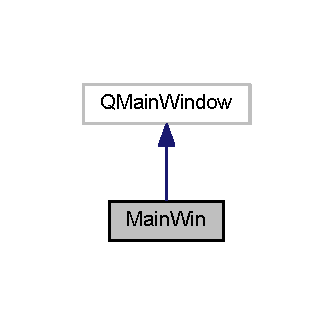
\includegraphics[width=160pt]{class_main_win__inherit__graph}
\end{center}
\end{figure}


Collaboration diagram for Main\-Win\-:\nopagebreak
\begin{figure}[H]
\begin{center}
\leavevmode
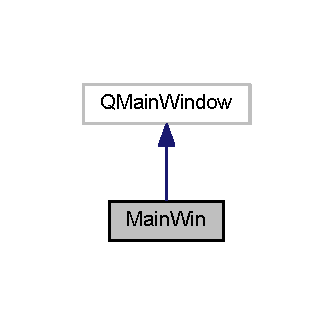
\includegraphics[width=160pt]{class_main_win__coll__graph}
\end{center}
\end{figure}
\subsection*{Public Member Functions}
\begin{DoxyCompactItemize}
\item 
\hypertarget{class_main_win_af05332e6fac4f7ab5c19b1a72aa7439d}{\hyperlink{class_main_win_af05332e6fac4f7ab5c19b1a72aa7439d}{Main\-Win} ()}\label{class_main_win_af05332e6fac4f7ab5c19b1a72aa7439d}

\begin{DoxyCompactList}\small\item\em Constructor. \end{DoxyCompactList}\item 
\hypertarget{class_main_win_a7068bb5ab02b75d4bbc78692388b9fb1}{\hyperlink{class_main_win_a7068bb5ab02b75d4bbc78692388b9fb1}{$\sim$\-Main\-Win} ()}\label{class_main_win_a7068bb5ab02b75d4bbc78692388b9fb1}

\begin{DoxyCompactList}\small\item\em Destructor. \end{DoxyCompactList}\item 
Q\-Size \hyperlink{class_main_win_af8f1854089c63efd6895ff536ad6ffc3}{size\-Hint} () const 
\begin{DoxyCompactList}\small\item\em Returns the desired size for when the window is created. \end{DoxyCompactList}\end{DoxyCompactItemize}
\subsection*{Protected Member Functions}
\begin{DoxyCompactItemize}
\item 
void \hyperlink{class_main_win_a06beabefe32c4e6514f76a07f1b63232}{close\-Event} (Q\-Close\-Event $\ast$event)
\begin{DoxyCompactList}\small\item\em Called when this window is closed\-: handles checking of log window. \end{DoxyCompactList}\end{DoxyCompactItemize}


\subsection{Detailed Description}
Application window class. 

Each \hyperlink{class_main_win}{Main\-Win} correcponds to exactly one currently open map document. If a new map document is created, it requires a new \hyperlink{class_main_win}{Main\-Win}. When the last \hyperlink{class_main_win}{Main\-Win} is closed, it will handle the closing of the log window if it is still open. 

\subsection{Member Function Documentation}
\hypertarget{class_main_win_a06beabefe32c4e6514f76a07f1b63232}{\index{Main\-Win@{Main\-Win}!close\-Event@{close\-Event}}
\index{close\-Event@{close\-Event}!MainWin@{Main\-Win}}
\subsubsection[{close\-Event}]{\setlength{\rightskip}{0pt plus 5cm}void Main\-Win\-::close\-Event (
\begin{DoxyParamCaption}
\item[{Q\-Close\-Event $\ast$}]{event}
\end{DoxyParamCaption}
)\hspace{0.3cm}{\ttfamily [protected]}}}\label{class_main_win_a06beabefe32c4e6514f76a07f1b63232}


Called when this window is closed\-: handles checking of log window. 


\begin{DoxyParams}{Parameters}
{\em event} & Close event. \\
\hline
\end{DoxyParams}
\hypertarget{class_main_win_af8f1854089c63efd6895ff536ad6ffc3}{\index{Main\-Win@{Main\-Win}!size\-Hint@{size\-Hint}}
\index{size\-Hint@{size\-Hint}!MainWin@{Main\-Win}}
\subsubsection[{size\-Hint}]{\setlength{\rightskip}{0pt plus 5cm}Q\-Size Main\-Win\-::size\-Hint (
\begin{DoxyParamCaption}
{}
\end{DoxyParamCaption}
) const\hspace{0.3cm}{\ttfamily [inline]}}}\label{class_main_win_af8f1854089c63efd6895ff536ad6ffc3}


Returns the desired size for when the window is created. 

\begin{DoxyReturn}{Returns}
Desired size. 
\end{DoxyReturn}


The documentation for this class was generated from the following files\-:\begin{DoxyCompactItemize}
\item 
app/\hyperlink{mainwin_8h}{mainwin.\-h}\item 
app/mainwin.\-cpp\end{DoxyCompactItemize}

\hypertarget{class_map_doc}{\section{Map\-Doc Class Reference}
\label{class_map_doc}\index{Map\-Doc@{Map\-Doc}}
}


The \hyperlink{class_map_doc}{Map\-Doc} class.  




{\ttfamily \#include $<$mapdoc.\-h$>$}



Inheritance diagram for Map\-Doc\-:
\nopagebreak
\begin{figure}[H]
\begin{center}
\leavevmode
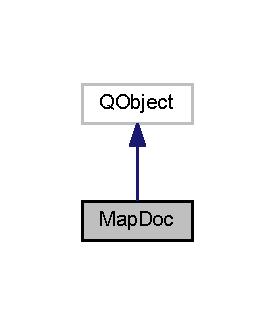
\includegraphics[width=132pt]{class_map_doc__inherit__graph}
\end{center}
\end{figure}


Collaboration diagram for Map\-Doc\-:
\nopagebreak
\begin{figure}[H]
\begin{center}
\leavevmode
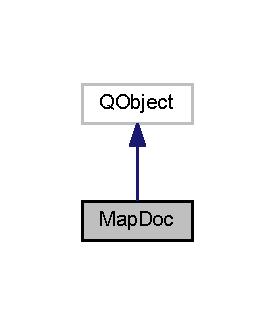
\includegraphics[width=132pt]{class_map_doc__coll__graph}
\end{center}
\end{figure}
\subsection*{Public Member Functions}
\begin{DoxyCompactItemize}
\item 
\hyperlink{class_map_doc_a2bea048c6b43333dc27fb4ca5ed84a95}{Map\-Doc} (Q\-Object $\ast$parent=0)
\begin{DoxyCompactList}\small\item\em Default constructor. \end{DoxyCompactList}\end{DoxyCompactItemize}
\subsection*{Static Public Member Functions}
\begin{DoxyCompactItemize}
\item 
static int \hyperlink{class_map_doc_a4bdaa5c5589e501d22a92f814f242b7c}{get\-Version} ()
\begin{DoxyCompactList}\small\item\em Gets the current version of the mapdoc. \end{DoxyCompactList}\end{DoxyCompactItemize}


\subsection{Detailed Description}
The \hyperlink{class_map_doc}{Map\-Doc} class. 

The \hyperlink{class_map_doc}{Map\-Doc} class details any information that will be serialised when a map source file is saved. This includes geometry and entities but also settings such as camera positions, grid size, snapping, etc. Geometry and entities are kept inside an octree that represents the entire 3\-D space in the level. 

\subsection{Constructor \& Destructor Documentation}
\hypertarget{class_map_doc_a2bea048c6b43333dc27fb4ca5ed84a95}{\index{Map\-Doc@{Map\-Doc}!Map\-Doc@{Map\-Doc}}
\index{Map\-Doc@{Map\-Doc}!MapDoc@{Map\-Doc}}
\subsubsection[{Map\-Doc}]{\setlength{\rightskip}{0pt plus 5cm}Map\-Doc\-::\-Map\-Doc (
\begin{DoxyParamCaption}
\item[{Q\-Object $\ast$}]{parent = {\ttfamily 0}}
\end{DoxyParamCaption}
)\hspace{0.3cm}{\ttfamily [explicit]}}}\label{class_map_doc_a2bea048c6b43333dc27fb4ca5ed84a95}


Default constructor. 


\begin{DoxyParams}{Parameters}
{\em parent} & Parent object. \\
\hline
\end{DoxyParams}


\subsection{Member Function Documentation}
\hypertarget{class_map_doc_a4bdaa5c5589e501d22a92f814f242b7c}{\index{Map\-Doc@{Map\-Doc}!get\-Version@{get\-Version}}
\index{get\-Version@{get\-Version}!MapDoc@{Map\-Doc}}
\subsubsection[{get\-Version}]{\setlength{\rightskip}{0pt plus 5cm}static int Map\-Doc\-::get\-Version (
\begin{DoxyParamCaption}
{}
\end{DoxyParamCaption}
)\hspace{0.3cm}{\ttfamily [inline]}, {\ttfamily [static]}}}\label{class_map_doc_a4bdaa5c5589e501d22a92f814f242b7c}


Gets the current version of the mapdoc. 

\begin{DoxyReturn}{Returns}
Mapdoc version. 
\end{DoxyReturn}


The documentation for this class was generated from the following files\-:\begin{DoxyCompactItemize}
\item 
app/\hyperlink{mapdoc_8h}{mapdoc.\-h}\item 
app/mapdoc.\-cpp\end{DoxyCompactItemize}

\hypertarget{class_plane}{\section{Plane Class Reference}
\label{class_plane}\index{Plane@{Plane}}
}


Defines a plane in 3\-D space.  




{\ttfamily \#include $<$plane.\-h$>$}

\subsection*{Public Member Functions}
\begin{DoxyCompactItemize}
\item 
\hypertarget{class_plane_acac0d9c003e0ab10d07b146c3566a0c7}{\hyperlink{class_plane_acac0d9c003e0ab10d07b146c3566a0c7}{Plane} ()}\label{class_plane_acac0d9c003e0ab10d07b146c3566a0c7}

\begin{DoxyCompactList}\small\item\em Constructor. Member variables are set to zero values. \end{DoxyCompactList}\item 
\hyperlink{class_plane_a044f4c5015112c8c5148ae28b41b8637}{Plane} (const Q\-Vector3\-D points\mbox{[}3\mbox{]})
\begin{DoxyCompactList}\small\item\em Constructor specifying an array of plane points. The normal is calculated with vectors \mbox{[}1\mbox{]}-\/\mbox{[}0\mbox{]}, \mbox{[}2\mbox{]}-\/\mbox{[}0\mbox{]}. \end{DoxyCompactList}\item 
\hyperlink{class_plane_affc3a1de45dcac9b65569eef3635eba4}{Plane} (const Q\-Vector3\-D p1, const Q\-Vector3\-D p2, const Q\-Vector3\-D p3)
\begin{DoxyCompactList}\small\item\em Constructor specifying plane points. The normal is calculated with vectors p2-\/p1, p3-\/p1. \end{DoxyCompactList}\item 
void \hyperlink{class_plane_af04d6d582cfc6bb3fdebfb7d2711c0b8}{get\-Points} (Q\-Vector3\-D points\mbox{[}3\mbox{]}) const 
\begin{DoxyCompactList}\small\item\em Gets an array of the three points on the plane. \end{DoxyCompactList}\item 
void \hyperlink{class_plane_ad8ca5183fed9db77a2cbb552d780aa9d}{get\-Points} (Q\-List$<$ Q\-Vector3\-D $>$ \&points) const 
\begin{DoxyCompactList}\small\item\em Fills a Q\-List with the three points on the plane. \end{DoxyCompactList}\item 
bool \hyperlink{class_plane_a9324f303beccf7ec9c6d3a5e371b7ca7}{is\-Valid} () const 
\begin{DoxyCompactList}\small\item\em Specifies whether the plane is valid. Invalid planes contain two or more identical plane points. \end{DoxyCompactList}\item 
Q\-Vector3\-D \hyperlink{class_plane_aeaae7bd417894c587423251818f16197}{get\-Normal} () const 
\begin{DoxyCompactList}\small\item\em Returns the plane's normal, specifying the forward-\/facing direction of the plane. \end{DoxyCompactList}\item 
void \hyperlink{class_plane_a3a9fd7ef1b74fad45bf0b18b93922813}{set\-Points} (const Q\-Vector3\-D points\mbox{[}3\mbox{]})
\begin{DoxyCompactList}\small\item\em Sets the plane's points via an array. The normal is calculated with vectors \mbox{[}1\mbox{]}-\/\mbox{[}0\mbox{]}, \mbox{[}2\mbox{]}-\/\mbox{[}0\mbox{]}. \end{DoxyCompactList}\item 
void \hyperlink{class_plane_ae4c5f7cda6d296b3cfccaac102471098}{set\-Points} (const Q\-List$<$ Q\-Vector3\-D $>$ \&points)
\begin{DoxyCompactList}\small\item\em Sets the plane's points via a Q\-List. The normal is calculated with vectors \mbox{[}1\mbox{]}-\/\mbox{[}0\mbox{]}, \mbox{[}2\mbox{]}-\/\mbox{[}0\mbox{]}. \end{DoxyCompactList}\item 
void \hyperlink{class_plane_a99ba0636ee74ea4cd8e5da15145b7c42}{set\-Points} (const Q\-Vector3\-D p1, const Q\-Vector3\-D p2, const Q\-Vector3\-D p3)
\begin{DoxyCompactList}\small\item\em Sets the plane's points. The normal is calculated with vectors p2-\/p1, p3-\/p1. \end{DoxyCompactList}\end{DoxyCompactItemize}


\subsection{Detailed Description}
Defines a plane in 3\-D space. 

\subsection{Constructor \& Destructor Documentation}
\hypertarget{class_plane_a044f4c5015112c8c5148ae28b41b8637}{\index{Plane@{Plane}!Plane@{Plane}}
\index{Plane@{Plane}!Plane@{Plane}}
\subsubsection[{Plane}]{\setlength{\rightskip}{0pt plus 5cm}Plane\-::\-Plane (
\begin{DoxyParamCaption}
\item[{const Q\-Vector3\-D}]{points\mbox{[}3\mbox{]}}
\end{DoxyParamCaption}
)\hspace{0.3cm}{\ttfamily [inline]}}}\label{class_plane_a044f4c5015112c8c5148ae28b41b8637}


Constructor specifying an array of plane points. The normal is calculated with vectors \mbox{[}1\mbox{]}-\/\mbox{[}0\mbox{]}, \mbox{[}2\mbox{]}-\/\mbox{[}0\mbox{]}. 


\begin{DoxyParams}{Parameters}
{\em points} & 3 points on the plane. \\
\hline
\end{DoxyParams}
\hypertarget{class_plane_affc3a1de45dcac9b65569eef3635eba4}{\index{Plane@{Plane}!Plane@{Plane}}
\index{Plane@{Plane}!Plane@{Plane}}
\subsubsection[{Plane}]{\setlength{\rightskip}{0pt plus 5cm}Plane\-::\-Plane (
\begin{DoxyParamCaption}
\item[{const Q\-Vector3\-D}]{p1, }
\item[{const Q\-Vector3\-D}]{p2, }
\item[{const Q\-Vector3\-D}]{p3}
\end{DoxyParamCaption}
)\hspace{0.3cm}{\ttfamily [inline]}}}\label{class_plane_affc3a1de45dcac9b65569eef3635eba4}


Constructor specifying plane points. The normal is calculated with vectors p2-\/p1, p3-\/p1. 


\begin{DoxyParams}{Parameters}
{\em p1} & Point 1. \\
\hline
{\em p2} & Point 2. \\
\hline
{\em p3} & Point 3. \\
\hline
\end{DoxyParams}


\subsection{Member Function Documentation}
\hypertarget{class_plane_aeaae7bd417894c587423251818f16197}{\index{Plane@{Plane}!get\-Normal@{get\-Normal}}
\index{get\-Normal@{get\-Normal}!Plane@{Plane}}
\subsubsection[{get\-Normal}]{\setlength{\rightskip}{0pt plus 5cm}Q\-Vector3\-D Plane\-::get\-Normal (
\begin{DoxyParamCaption}
{}
\end{DoxyParamCaption}
) const\hspace{0.3cm}{\ttfamily [inline]}}}\label{class_plane_aeaae7bd417894c587423251818f16197}


Returns the plane's normal, specifying the forward-\/facing direction of the plane. 

\begin{DoxyReturn}{Returns}
Normalised direction vector representing the plane's normal. 
\end{DoxyReturn}
\hypertarget{class_plane_af04d6d582cfc6bb3fdebfb7d2711c0b8}{\index{Plane@{Plane}!get\-Points@{get\-Points}}
\index{get\-Points@{get\-Points}!Plane@{Plane}}
\subsubsection[{get\-Points}]{\setlength{\rightskip}{0pt plus 5cm}void Plane\-::get\-Points (
\begin{DoxyParamCaption}
\item[{Q\-Vector3\-D}]{points\mbox{[}3\mbox{]}}
\end{DoxyParamCaption}
) const\hspace{0.3cm}{\ttfamily [inline]}}}\label{class_plane_af04d6d582cfc6bb3fdebfb7d2711c0b8}


Gets an array of the three points on the plane. 


\begin{DoxyParams}{Parameters}
{\em points} & Array to fill with points. \\
\hline
\end{DoxyParams}
\hypertarget{class_plane_ad8ca5183fed9db77a2cbb552d780aa9d}{\index{Plane@{Plane}!get\-Points@{get\-Points}}
\index{get\-Points@{get\-Points}!Plane@{Plane}}
\subsubsection[{get\-Points}]{\setlength{\rightskip}{0pt plus 5cm}void Plane\-::get\-Points (
\begin{DoxyParamCaption}
\item[{Q\-List$<$ Q\-Vector3\-D $>$ \&}]{points}
\end{DoxyParamCaption}
) const\hspace{0.3cm}{\ttfamily [inline]}}}\label{class_plane_ad8ca5183fed9db77a2cbb552d780aa9d}


Fills a Q\-List with the three points on the plane. 


\begin{DoxyParams}{Parameters}
{\em points} & List to fill. Points are appended to the list. \\
\hline
\end{DoxyParams}
\hypertarget{class_plane_a9324f303beccf7ec9c6d3a5e371b7ca7}{\index{Plane@{Plane}!is\-Valid@{is\-Valid}}
\index{is\-Valid@{is\-Valid}!Plane@{Plane}}
\subsubsection[{is\-Valid}]{\setlength{\rightskip}{0pt plus 5cm}bool Plane\-::is\-Valid (
\begin{DoxyParamCaption}
{}
\end{DoxyParamCaption}
) const\hspace{0.3cm}{\ttfamily [inline]}}}\label{class_plane_a9324f303beccf7ec9c6d3a5e371b7ca7}


Specifies whether the plane is valid. Invalid planes contain two or more identical plane points. 

\begin{DoxyReturn}{Returns}
True if valid, false otherwise. 
\end{DoxyReturn}
\hypertarget{class_plane_a3a9fd7ef1b74fad45bf0b18b93922813}{\index{Plane@{Plane}!set\-Points@{set\-Points}}
\index{set\-Points@{set\-Points}!Plane@{Plane}}
\subsubsection[{set\-Points}]{\setlength{\rightskip}{0pt plus 5cm}void Plane\-::set\-Points (
\begin{DoxyParamCaption}
\item[{const Q\-Vector3\-D}]{points\mbox{[}3\mbox{]}}
\end{DoxyParamCaption}
)}}\label{class_plane_a3a9fd7ef1b74fad45bf0b18b93922813}


Sets the plane's points via an array. The normal is calculated with vectors \mbox{[}1\mbox{]}-\/\mbox{[}0\mbox{]}, \mbox{[}2\mbox{]}-\/\mbox{[}0\mbox{]}. 


\begin{DoxyParams}{Parameters}
{\em points} & Array of points to set. \\
\hline
\end{DoxyParams}
\hypertarget{class_plane_ae4c5f7cda6d296b3cfccaac102471098}{\index{Plane@{Plane}!set\-Points@{set\-Points}}
\index{set\-Points@{set\-Points}!Plane@{Plane}}
\subsubsection[{set\-Points}]{\setlength{\rightskip}{0pt plus 5cm}void Plane\-::set\-Points (
\begin{DoxyParamCaption}
\item[{const Q\-List$<$ Q\-Vector3\-D $>$ \&}]{points}
\end{DoxyParamCaption}
)}}\label{class_plane_ae4c5f7cda6d296b3cfccaac102471098}


Sets the plane's points via a Q\-List. The normal is calculated with vectors \mbox{[}1\mbox{]}-\/\mbox{[}0\mbox{]}, \mbox{[}2\mbox{]}-\/\mbox{[}0\mbox{]}. 


\begin{DoxyParams}{Parameters}
{\em points} & List of points to set. \\
\hline
\end{DoxyParams}
\hypertarget{class_plane_a99ba0636ee74ea4cd8e5da15145b7c42}{\index{Plane@{Plane}!set\-Points@{set\-Points}}
\index{set\-Points@{set\-Points}!Plane@{Plane}}
\subsubsection[{set\-Points}]{\setlength{\rightskip}{0pt plus 5cm}void Plane\-::set\-Points (
\begin{DoxyParamCaption}
\item[{const Q\-Vector3\-D}]{p1, }
\item[{const Q\-Vector3\-D}]{p2, }
\item[{const Q\-Vector3\-D}]{p3}
\end{DoxyParamCaption}
)}}\label{class_plane_a99ba0636ee74ea4cd8e5da15145b7c42}


Sets the plane's points. The normal is calculated with vectors p2-\/p1, p3-\/p1. 


\begin{DoxyParams}{Parameters}
{\em p1} & First point. \\
\hline
{\em p2} & Second point. \\
\hline
{\em p3} & Third point. \\
\hline
\end{DoxyParams}


The documentation for this class was generated from the following files\-:\begin{DoxyCompactItemize}
\item 
app/\hyperlink{plane_8h}{plane.\-h}\item 
app/plane.\-cpp\end{DoxyCompactItemize}

\hypertarget{class_plugin_manager}{\section{Plugin\-Manager Class Reference}
\label{class_plugin_manager}\index{Plugin\-Manager@{Plugin\-Manager}}
}


Manages loading of plugins.  




{\ttfamily \#include $<$pluginmanager.\-h$>$}



Inheritance diagram for Plugin\-Manager\-:
\nopagebreak
\begin{figure}[H]
\begin{center}
\leavevmode
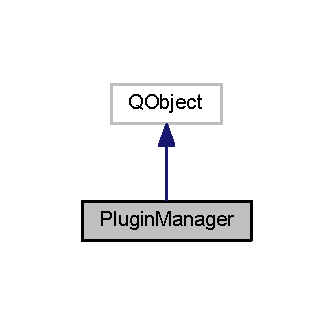
\includegraphics[width=160pt]{class_plugin_manager__inherit__graph}
\end{center}
\end{figure}


Collaboration diagram for Plugin\-Manager\-:
\nopagebreak
\begin{figure}[H]
\begin{center}
\leavevmode
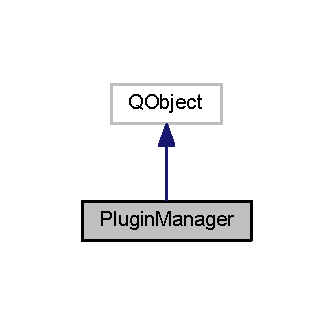
\includegraphics[width=160pt]{class_plugin_manager__coll__graph}
\end{center}
\end{figure}
\subsection*{Public Slots}
\begin{DoxyCompactItemize}
\item 
void \hyperlink{class_plugin_manager_a2e8795656b18a1ff483f2d7a4a6b7988}{Set\-Load\-Dir} (Q\-String dir)
\begin{DoxyCompactList}\small\item\em Sets the directory from which to load plugins. \end{DoxyCompactList}\end{DoxyCompactItemize}
\subsection*{Public Member Functions}
\begin{DoxyCompactItemize}
\item 
\hyperlink{class_plugin_manager_aac3752227a8bdae34eada08e6b80c3ce}{Plugin\-Manager} (Q\-Object $\ast$parent=0, Q\-String load\-Dir=\char`\"{}\char`\"{})
\begin{DoxyCompactList}\small\item\em Constructor. \end{DoxyCompactList}\item 
\hypertarget{class_plugin_manager_ab657302ef5af357907ae11ad817f5dfc}{\hyperlink{class_plugin_manager_ab657302ef5af357907ae11ad817f5dfc}{$\sim$\-Plugin\-Manager} ()}\label{class_plugin_manager_ab657302ef5af357907ae11ad817f5dfc}

\begin{DoxyCompactList}\small\item\em Destructor. \end{DoxyCompactList}\item 
Q\-List$<$ Q\-String $>$ \hyperlink{class_plugin_manager_a31f3817b1f01dac04059827dc0fe37f7}{Load\-Plugins} ()
\begin{DoxyCompactList}\small\item\em Loads plugins and returns a list of I\-Ds for those successfully loaded. \end{DoxyCompactList}\end{DoxyCompactItemize}
\subsection*{Protected Member Functions}
\begin{DoxyCompactItemize}
\item 
\hypertarget{class_plugin_manager_a7299c68a352c5fde51e803b32828b3da}{void \hyperlink{class_plugin_manager_a7299c68a352c5fde51e803b32828b3da}{Delete\-Plugin\-List} ()}\label{class_plugin_manager_a7299c68a352c5fde51e803b32828b3da}

\begin{DoxyCompactList}\small\item\em Destroys all plugins in the hash table. \end{DoxyCompactList}\item 
Q\-Dir \hyperlink{class_plugin_manager_a08a9b22dabdc191e7ce173c8fca93821}{Full\-Plugin\-Path} ()
\begin{DoxyCompactList}\small\item\em Generates full path from given plugin load directory. \end{DoxyCompactList}\end{DoxyCompactItemize}
\subsection*{Protected Attributes}
\begin{DoxyCompactItemize}
\item 
Q\-String \hyperlink{class_plugin_manager_ad76c45e41d41eac52be4ba19e4ae11fb}{m\-\_\-sz\-Load\-Dir}
\item 
Q\-Hash$<$ Q\-String, Q\-Object $\ast$ $>$ $\ast$ \hyperlink{class_plugin_manager_af65cae6069dfdb469aee42c4d2ec94d2}{m\-\_\-\-Plugin\-List}
\end{DoxyCompactItemize}


\subsection{Detailed Description}
Manages loading of plugins. 

\subsection{Constructor \& Destructor Documentation}
\hypertarget{class_plugin_manager_aac3752227a8bdae34eada08e6b80c3ce}{\index{Plugin\-Manager@{Plugin\-Manager}!Plugin\-Manager@{Plugin\-Manager}}
\index{Plugin\-Manager@{Plugin\-Manager}!PluginManager@{Plugin\-Manager}}
\subsubsection[{Plugin\-Manager}]{\setlength{\rightskip}{0pt plus 5cm}Plugin\-Manager\-::\-Plugin\-Manager (
\begin{DoxyParamCaption}
\item[{Q\-Object $\ast$}]{parent = {\ttfamily 0}, }
\item[{Q\-String}]{load\-Dir = {\ttfamily \char`\"{}\char`\"{}}}
\end{DoxyParamCaption}
)\hspace{0.3cm}{\ttfamily [explicit]}}}\label{class_plugin_manager_aac3752227a8bdae34eada08e6b80c3ce}


Constructor. 


\begin{DoxyParams}{Parameters}
{\em parent} & Parent object (usually N\-U\-L\-L). \\
\hline
{\em load\-Dir} & Directory from which to load plugins, relative to the application directory. \\
\hline
\end{DoxyParams}


\subsection{Member Function Documentation}
\hypertarget{class_plugin_manager_a08a9b22dabdc191e7ce173c8fca93821}{\index{Plugin\-Manager@{Plugin\-Manager}!Full\-Plugin\-Path@{Full\-Plugin\-Path}}
\index{Full\-Plugin\-Path@{Full\-Plugin\-Path}!PluginManager@{Plugin\-Manager}}
\subsubsection[{Full\-Plugin\-Path}]{\setlength{\rightskip}{0pt plus 5cm}Q\-Dir Plugin\-Manager\-::\-Full\-Plugin\-Path (
\begin{DoxyParamCaption}
{}
\end{DoxyParamCaption}
)\hspace{0.3cm}{\ttfamily [protected]}}}\label{class_plugin_manager_a08a9b22dabdc191e7ce173c8fca93821}


Generates full path from given plugin load directory. 

\begin{DoxyNote}{Note}
If the path does not exist, the returned path will be the application directory. 
\end{DoxyNote}
\begin{DoxyReturn}{Returns}
Full path of application and load directory. 
\end{DoxyReturn}
\hypertarget{class_plugin_manager_a31f3817b1f01dac04059827dc0fe37f7}{\index{Plugin\-Manager@{Plugin\-Manager}!Load\-Plugins@{Load\-Plugins}}
\index{Load\-Plugins@{Load\-Plugins}!PluginManager@{Plugin\-Manager}}
\subsubsection[{Load\-Plugins}]{\setlength{\rightskip}{0pt plus 5cm}Q\-List$<$ Q\-String $>$ Plugin\-Manager\-::\-Load\-Plugins (
\begin{DoxyParamCaption}
{}
\end{DoxyParamCaption}
)}}\label{class_plugin_manager_a31f3817b1f01dac04059827dc0fe37f7}


Loads plugins and returns a list of I\-Ds for those successfully loaded. 

\begin{DoxyReturn}{Returns}
List of successfully loaded plugins. 
\end{DoxyReturn}
\hypertarget{class_plugin_manager_a2e8795656b18a1ff483f2d7a4a6b7988}{\index{Plugin\-Manager@{Plugin\-Manager}!Set\-Load\-Dir@{Set\-Load\-Dir}}
\index{Set\-Load\-Dir@{Set\-Load\-Dir}!PluginManager@{Plugin\-Manager}}
\subsubsection[{Set\-Load\-Dir}]{\setlength{\rightskip}{0pt plus 5cm}void Plugin\-Manager\-::\-Set\-Load\-Dir (
\begin{DoxyParamCaption}
\item[{Q\-String}]{dir}
\end{DoxyParamCaption}
)\hspace{0.3cm}{\ttfamily [inline]}, {\ttfamily [slot]}}}\label{class_plugin_manager_a2e8795656b18a1ff483f2d7a4a6b7988}


Sets the directory from which to load plugins. 


\begin{DoxyParams}{Parameters}
{\em dir} & Directory path relative to the application directory. \\
\hline
\end{DoxyParams}


\subsection{Member Data Documentation}
\hypertarget{class_plugin_manager_af65cae6069dfdb469aee42c4d2ec94d2}{\index{Plugin\-Manager@{Plugin\-Manager}!m\-\_\-\-Plugin\-List@{m\-\_\-\-Plugin\-List}}
\index{m\-\_\-\-Plugin\-List@{m\-\_\-\-Plugin\-List}!PluginManager@{Plugin\-Manager}}
\subsubsection[{m\-\_\-\-Plugin\-List}]{\setlength{\rightskip}{0pt plus 5cm}Q\-Hash$<$Q\-String, Q\-Object$\ast$$>$$\ast$ Plugin\-Manager\-::m\-\_\-\-Plugin\-List\hspace{0.3cm}{\ttfamily [protected]}}}\label{class_plugin_manager_af65cae6069dfdb469aee42c4d2ec94d2}
List of all loaded plugins. \hypertarget{class_plugin_manager_ad76c45e41d41eac52be4ba19e4ae11fb}{\index{Plugin\-Manager@{Plugin\-Manager}!m\-\_\-sz\-Load\-Dir@{m\-\_\-sz\-Load\-Dir}}
\index{m\-\_\-sz\-Load\-Dir@{m\-\_\-sz\-Load\-Dir}!PluginManager@{Plugin\-Manager}}
\subsubsection[{m\-\_\-sz\-Load\-Dir}]{\setlength{\rightskip}{0pt plus 5cm}Q\-String Plugin\-Manager\-::m\-\_\-sz\-Load\-Dir\hspace{0.3cm}{\ttfamily [protected]}}}\label{class_plugin_manager_ad76c45e41d41eac52be4ba19e4ae11fb}
Path to load plugins from. 

The documentation for this class was generated from the following files\-:\begin{DoxyCompactItemize}
\item 
app/\hyperlink{pluginmanager_8h}{pluginmanager.\-h}\item 
app/pluginmanager.\-cpp\end{DoxyCompactItemize}

\hypertarget{class_solid3_d}{\section{Solid3\-D Class Reference}
\label{class_solid3_d}\index{Solid3\-D@{Solid3\-D}}
}


Class representing a 3\-D solid.  




{\ttfamily \#include $<$solid.\-h$>$}



Inheritance diagram for Solid3\-D\-:\nopagebreak
\begin{figure}[H]
\begin{center}
\leavevmode
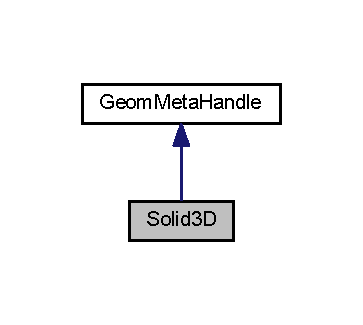
\includegraphics[width=174pt]{class_solid3_d__inherit__graph}
\end{center}
\end{figure}


Collaboration diagram for Solid3\-D\-:\nopagebreak
\begin{figure}[H]
\begin{center}
\leavevmode
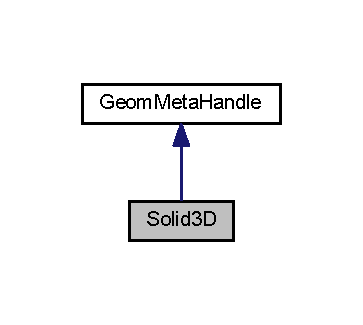
\includegraphics[width=174pt]{class_solid3_d__coll__graph}
\end{center}
\end{figure}
\subsection*{Public Types}
\begin{DoxyCompactItemize}
\item 
enum \{ \hyperlink{class_solid3_d_a85c6b265036f308d59f14a1945419de3a0bc5c527e2f2681822af8cdbe91f13cb}{M\-A\-X\-\_\-\-V\-E\-R\-T\-I\-C\-E\-S} = 384, 
\hyperlink{class_solid3_d_a85c6b265036f308d59f14a1945419de3adea5e83841760466066bb7ef63f9779f}{M\-A\-X\-\_\-\-E\-D\-G\-E\-S} = 384, 
\hyperlink{class_solid3_d_a85c6b265036f308d59f14a1945419de3a85c95a8842482e9e0db2f3c6ff68f19a}{M\-A\-X\-\_\-\-F\-A\-C\-E\-S} = 384
 \}
\item 
\hypertarget{class_solid3_d_acaa1c40fc6c74ee5c77e64baa3a672b1}{typedef Q\-Vector$<$ \hyperlink{class_vertex3_d}{Vertex3\-D} $\ast$ $>$ \hyperlink{class_solid3_d_acaa1c40fc6c74ee5c77e64baa3a672b1}{Vertex3\-D\-List}}\label{class_solid3_d_acaa1c40fc6c74ee5c77e64baa3a672b1}

\begin{DoxyCompactList}\small\item\em Vertex3\-D\-List typedef. \end{DoxyCompactList}\item 
\hypertarget{class_solid3_d_ac9b57b2279aeedb1dc657ac13271727b}{typedef Q\-Vector$<$ \hyperlink{class_edge3_d}{Edge3\-D} $\ast$ $>$ \hyperlink{class_solid3_d_ac9b57b2279aeedb1dc657ac13271727b}{Edge3\-D\-List}}\label{class_solid3_d_ac9b57b2279aeedb1dc657ac13271727b}

\begin{DoxyCompactList}\small\item\em Edge3\-D\-List typedef. \end{DoxyCompactList}\item 
\hypertarget{class_solid3_d_afd4862e0f4b30967e6f0cb2013ccc084}{typedef Q\-Vector$<$ \hyperlink{class_face3_d}{Face3\-D} $\ast$ $>$ \hyperlink{class_solid3_d_afd4862e0f4b30967e6f0cb2013ccc084}{Face3\-D\-List}}\label{class_solid3_d_afd4862e0f4b30967e6f0cb2013ccc084}

\begin{DoxyCompactList}\small\item\em Face3\-D\-List typedef. \end{DoxyCompactList}\end{DoxyCompactItemize}
\subsection*{Public Member Functions}
\begin{DoxyCompactItemize}
\item 
\hypertarget{class_solid3_d_a8c69dd01b422d74c8ff298e7f9ba95d5}{\hyperlink{class_solid3_d_a8c69dd01b422d74c8ff298e7f9ba95d5}{Solid3\-D} ()}\label{class_solid3_d_a8c69dd01b422d74c8ff298e7f9ba95d5}

\begin{DoxyCompactList}\small\item\em Default constructor. Initialises empty members. \end{DoxyCompactList}\item 
\hypertarget{class_solid3_d_afa6ecd2e276b4ef5a09f3c660a6ccfed}{\hyperlink{class_solid3_d_afa6ecd2e276b4ef5a09f3c660a6ccfed}{$\sim$\-Solid3\-D} ()}\label{class_solid3_d_afa6ecd2e276b4ef5a09f3c660a6ccfed}

\begin{DoxyCompactList}\small\item\em Destructor. \end{DoxyCompactList}\item 
bool \hyperlink{class_solid3_d_ac02ad8ea1ca4d970c77ddc4c09b043cc}{add\-Vertex} (\hyperlink{class_vertex3_d}{Vertex3\-D} $\ast$vertex)
\begin{DoxyCompactList}\small\item\em Adds the specified vertex. \end{DoxyCompactList}\item 
\hyperlink{class_vertex3_d}{Vertex3\-D} $\ast$ \hyperlink{class_solid3_d_aefadc03bef752b5eeb52e80d67074980}{remove\-Vertex\-Handle} (const \hyperlink{vertex_8h_a72202e57358ed73cd212e9a2eaf39aeb}{G\-E\-O\-M\-H\-A\-N\-D\-L\-E} vertex)
\begin{DoxyCompactList}\small\item\em Removes the vertex with the specified handle. \end{DoxyCompactList}\item 
\hyperlink{class_vertex3_d}{Vertex3\-D} $\ast$ \hyperlink{class_solid3_d_ace3ab2ef41ff561973c10253b18add81}{find\-Vertex} (const \hyperlink{vertex_8h_a72202e57358ed73cd212e9a2eaf39aeb}{G\-E\-O\-M\-H\-A\-N\-D\-L\-E} vertex) const 
\begin{DoxyCompactList}\small\item\em Returns a pointer to the vertex with the specified handle. \end{DoxyCompactList}\item 
void \hyperlink{class_solid3_d_aa250bf5e45c3890a031ee7d10fd0a495}{find\-Related\-Edges\-For\-Vertex} (Q\-List$<$ \hyperlink{vertex_8h_a72202e57358ed73cd212e9a2eaf39aeb}{G\-E\-O\-M\-H\-A\-N\-D\-L\-E} $>$ \&out\-Edges, \hyperlink{vertex_8h_a72202e57358ed73cd212e9a2eaf39aeb}{G\-E\-O\-M\-H\-A\-N\-D\-L\-E} vertex)
\begin{DoxyCompactList}\small\item\em Finds all edges whose start or end vertices reference the given vertex handle. \end{DoxyCompactList}\item 
void \hyperlink{class_solid3_d_a84f5c532f14916e59ba99b339e19975e}{find\-Related\-Edges\-For\-Vertex} (Q\-List$<$ \hyperlink{vertex_8h_a72202e57358ed73cd212e9a2eaf39aeb}{G\-E\-O\-M\-H\-A\-N\-D\-L\-E} $>$ \&out\-Edges, Q\-List$<$ \hyperlink{vertex_8h_a72202e57358ed73cd212e9a2eaf39aeb}{G\-E\-O\-M\-H\-A\-N\-D\-L\-E} $>$ \&vertices)
\begin{DoxyCompactList}\small\item\em Finds all edges whose start or end vertices reference any of the given vertex handles. \end{DoxyCompactList}\item 
void \hyperlink{class_solid3_d_a00bfad9d7e6dbe5ff290074753329e92}{find\-Related\-Faces\-For\-Vertex} (Q\-List$<$ \hyperlink{vertex_8h_a72202e57358ed73cd212e9a2eaf39aeb}{G\-E\-O\-M\-H\-A\-N\-D\-L\-E} $>$ \&out\-Faces, \hyperlink{vertex_8h_a72202e57358ed73cd212e9a2eaf39aeb}{G\-E\-O\-M\-H\-A\-N\-D\-L\-E} vertex)
\begin{DoxyCompactList}\small\item\em Finds all faces whose edges reference the given vertex handle. \end{DoxyCompactList}\item 
void \hyperlink{class_solid3_d_ac2b735d2b9ee6e47f56b49e4b122582c}{find\-Related\-Faces\-For\-Vertex} (Q\-List$<$ \hyperlink{vertex_8h_a72202e57358ed73cd212e9a2eaf39aeb}{G\-E\-O\-M\-H\-A\-N\-D\-L\-E} $>$ \&out\-Faces, Q\-List$<$ \hyperlink{vertex_8h_a72202e57358ed73cd212e9a2eaf39aeb}{G\-E\-O\-M\-H\-A\-N\-D\-L\-E} $>$ \&vertices)
\begin{DoxyCompactList}\small\item\em Finds all faces whose edges reference any of the given vertex handles. \end{DoxyCompactList}\item 
bool \hyperlink{class_solid3_d_aad6d7269dbea23a025ba3f598183bc22}{add\-Edge} (\hyperlink{class_edge3_d}{Edge3\-D} $\ast$edge)
\begin{DoxyCompactList}\small\item\em Adds the specified edge. \end{DoxyCompactList}\item 
\hyperlink{class_edge3_d}{Edge3\-D} $\ast$ \hyperlink{class_solid3_d_a3874333554e5105e789e06de3accb9d5}{remove\-Edge\-Handle} (const \hyperlink{vertex_8h_a72202e57358ed73cd212e9a2eaf39aeb}{G\-E\-O\-M\-H\-A\-N\-D\-L\-E} edge)
\begin{DoxyCompactList}\small\item\em Removes the edge with the specified handle. \end{DoxyCompactList}\item 
\hyperlink{class_edge3_d}{Edge3\-D} $\ast$ \hyperlink{class_solid3_d_ab5a26fa3df1a830f972bd3a57d412a08}{find\-Edge} (const \hyperlink{vertex_8h_a72202e57358ed73cd212e9a2eaf39aeb}{G\-E\-O\-M\-H\-A\-N\-D\-L\-E} edge) const 
\begin{DoxyCompactList}\small\item\em Returns a pointer to the edge with the specified handle. \end{DoxyCompactList}\item 
void \hyperlink{class_solid3_d_a3a7ce9251333f2ff387292d229ac4aa5}{find\-Related\-Faces\-For\-Edge} (Q\-List$<$ \hyperlink{vertex_8h_a72202e57358ed73cd212e9a2eaf39aeb}{G\-E\-O\-M\-H\-A\-N\-D\-L\-E} $>$ \&out\-Faces, \hyperlink{vertex_8h_a72202e57358ed73cd212e9a2eaf39aeb}{G\-E\-O\-M\-H\-A\-N\-D\-L\-E} edge)
\begin{DoxyCompactList}\small\item\em Finds all faces which contain the given edge. \end{DoxyCompactList}\item 
void \hyperlink{class_solid3_d_aa388640fa5cf2fb0e94630f5480f024e}{find\-Related\-Faces\-For\-Edge} (Q\-List$<$ \hyperlink{vertex_8h_a72202e57358ed73cd212e9a2eaf39aeb}{G\-E\-O\-M\-H\-A\-N\-D\-L\-E} $>$ \&out\-Faces, Q\-List$<$ \hyperlink{vertex_8h_a72202e57358ed73cd212e9a2eaf39aeb}{G\-E\-O\-M\-H\-A\-N\-D\-L\-E} $>$ \&edges)
\begin{DoxyCompactList}\small\item\em Finds all faces which contain any of the given edges. \end{DoxyCompactList}\item 
bool \hyperlink{class_solid3_d_a3976c227473c5954bfac9e2edf4078ea}{add\-Face} (\hyperlink{class_face3_d}{Face3\-D} $\ast$face)
\begin{DoxyCompactList}\small\item\em Adds the specified face. \end{DoxyCompactList}\item 
\hyperlink{class_face3_d}{Face3\-D} $\ast$ \hyperlink{class_solid3_d_a49bec433727595c0aa5fef4097e9d6b2}{remove\-Face\-Handle} (const \hyperlink{vertex_8h_a72202e57358ed73cd212e9a2eaf39aeb}{G\-E\-O\-M\-H\-A\-N\-D\-L\-E} face)
\begin{DoxyCompactList}\small\item\em Removes the face with the specified handle. \end{DoxyCompactList}\item 
\hyperlink{class_face3_d}{Face3\-D} $\ast$ \hyperlink{class_solid3_d_af1e9c9e9c969f7f935296c3706e8f08f}{find\-Face} (const \hyperlink{vertex_8h_a72202e57358ed73cd212e9a2eaf39aeb}{G\-E\-O\-M\-H\-A\-N\-D\-L\-E} face) const 
\begin{DoxyCompactList}\small\item\em Returns a pointer to the face with the specified handle. \end{DoxyCompactList}\item 
void \hyperlink{class_solid3_d_a844ed140f035f5cbeb325687d10e9d32}{identify\-Handle} (\hyperlink{vertex_8h_a72202e57358ed73cd212e9a2eaf39aeb}{G\-E\-O\-M\-H\-A\-N\-D\-L\-E} handle, \hyperlink{struct_geom_info}{Geom\-Info} \&info) const 
\begin{DoxyCompactList}\small\item\em Outputs information about the given geometry component to the \hyperlink{struct_geom_info}{Geom\-Info} struct. \end{DoxyCompactList}\item 
const \hyperlink{class_solid3_d_acaa1c40fc6c74ee5c77e64baa3a672b1}{Vertex3\-D\-List} \& \hyperlink{class_solid3_d_aa97775f007b84f89802d1f87b24665a0}{get\-Vertex\-List} () const 
\begin{DoxyCompactList}\small\item\em Returns the vertex list. \end{DoxyCompactList}\item 
const \hyperlink{class_solid3_d_ac9b57b2279aeedb1dc657ac13271727b}{Edge3\-D\-List} \& \hyperlink{class_solid3_d_ab0937f1a2d79a4ae72fcafb7b9f4ab7d}{get\-Edge\-List} () const 
\begin{DoxyCompactList}\small\item\em Returns the edge list. \end{DoxyCompactList}\item 
const \hyperlink{class_solid3_d_afd4862e0f4b30967e6f0cb2013ccc084}{Face3\-D\-List} \& \hyperlink{class_solid3_d_a17968c6a8e59d14268240ff1548cc51d}{get\-Face\-List} () const 
\begin{DoxyCompactList}\small\item\em Returns the face list. \end{DoxyCompactList}\item 
\hyperlink{vertex_8h_a72202e57358ed73cd212e9a2eaf39aeb}{G\-E\-O\-M\-H\-A\-N\-D\-L\-E} \hyperlink{class_solid3_d_ac2fda07777d7c7a856add07ceb24c395}{get\-Handle} () const 
\begin{DoxyCompactList}\small\item\em Returns this solid's handle. \end{DoxyCompactList}\item 
void \hyperlink{class_solid3_d_ab12674813ab277a7c4dac092367da6cd}{set\-Handle} (const \hyperlink{vertex_8h_a72202e57358ed73cd212e9a2eaf39aeb}{G\-E\-O\-M\-H\-A\-N\-D\-L\-E} handle)
\begin{DoxyCompactList}\small\item\em Sets this solid's handle. \end{DoxyCompactList}\end{DoxyCompactItemize}
\subsection*{Additional Inherited Members}


\subsection{Detailed Description}
Class representing a 3\-D solid. 

Solids are the programmatical implementation of brushes and are made up of sets of vertices, edges and faces. Each edge references the vertices it links, and each face is built from multiple edges. As opposed to Hammer's implementation, solids are mesh-\/based (ie. they are defined by vertex positions and links rather than planes and intersections) to allow for easier manipulation, and are exported as plane-\/based objects when serialised as a V\-M\-F.\par
 It is recommended to work {\bfseries bottom-\/up} (ie. add any required vertices before edges, and edges before faces) rather than {\bfseries top-\/down} (creating all of a face's edges and vertices as the face itself is created) as the former method is less prone to errors. 

\subsection{Member Enumeration Documentation}
\hypertarget{class_solid3_d_a85c6b265036f308d59f14a1945419de3}{\subsubsection[{anonymous enum}]{\setlength{\rightskip}{0pt plus 5cm}anonymous enum}}\label{class_solid3_d_a85c6b265036f308d59f14a1945419de3}
\begin{Desc}
\item[Enumerator]\par
\begin{description}
\index{M\-A\-X\-\_\-\-V\-E\-R\-T\-I\-C\-E\-S@{M\-A\-X\-\_\-\-V\-E\-R\-T\-I\-C\-E\-S}!Solid3\-D@{Solid3\-D}}\index{Solid3\-D@{Solid3\-D}!M\-A\-X\-\_\-\-V\-E\-R\-T\-I\-C\-E\-S@{M\-A\-X\-\_\-\-V\-E\-R\-T\-I\-C\-E\-S}}\item[{\em 
\hypertarget{class_solid3_d_a85c6b265036f308d59f14a1945419de3a0bc5c527e2f2681822af8cdbe91f13cb}{M\-A\-X\-\_\-\-V\-E\-R\-T\-I\-C\-E\-S}\label{class_solid3_d_a85c6b265036f308d59f14a1945419de3a0bc5c527e2f2681822af8cdbe91f13cb}
}]Max vertices allowed in a solid. \index{M\-A\-X\-\_\-\-E\-D\-G\-E\-S@{M\-A\-X\-\_\-\-E\-D\-G\-E\-S}!Solid3\-D@{Solid3\-D}}\index{Solid3\-D@{Solid3\-D}!M\-A\-X\-\_\-\-E\-D\-G\-E\-S@{M\-A\-X\-\_\-\-E\-D\-G\-E\-S}}\item[{\em 
\hypertarget{class_solid3_d_a85c6b265036f308d59f14a1945419de3adea5e83841760466066bb7ef63f9779f}{M\-A\-X\-\_\-\-E\-D\-G\-E\-S}\label{class_solid3_d_a85c6b265036f308d59f14a1945419de3adea5e83841760466066bb7ef63f9779f}
}]Max edges allowed in a solid. \index{M\-A\-X\-\_\-\-F\-A\-C\-E\-S@{M\-A\-X\-\_\-\-F\-A\-C\-E\-S}!Solid3\-D@{Solid3\-D}}\index{Solid3\-D@{Solid3\-D}!M\-A\-X\-\_\-\-F\-A\-C\-E\-S@{M\-A\-X\-\_\-\-F\-A\-C\-E\-S}}\item[{\em 
\hypertarget{class_solid3_d_a85c6b265036f308d59f14a1945419de3a85c95a8842482e9e0db2f3c6ff68f19a}{M\-A\-X\-\_\-\-F\-A\-C\-E\-S}\label{class_solid3_d_a85c6b265036f308d59f14a1945419de3a85c95a8842482e9e0db2f3c6ff68f19a}
}]Max faces allowed in a solid. \end{description}
\end{Desc}


\subsection{Member Function Documentation}
\hypertarget{class_solid3_d_aad6d7269dbea23a025ba3f598183bc22}{\index{Solid3\-D@{Solid3\-D}!add\-Edge@{add\-Edge}}
\index{add\-Edge@{add\-Edge}!Solid3D@{Solid3\-D}}
\subsubsection[{add\-Edge}]{\setlength{\rightskip}{0pt plus 5cm}bool Solid3\-D\-::add\-Edge (
\begin{DoxyParamCaption}
\item[{{\bf Edge3\-D} $\ast$}]{edge}
\end{DoxyParamCaption}
)}}\label{class_solid3_d_aad6d7269dbea23a025ba3f598183bc22}


Adds the specified edge. 

The edge's handles will be updated to reflect its place in the solid. 
\begin{DoxyParams}{Parameters}
{\em edge} & Edge to add. \\
\hline
\end{DoxyParams}
\begin{DoxyReturn}{Returns}
True if addition was successful, false if it was not. 
\end{DoxyReturn}
\hypertarget{class_solid3_d_a3976c227473c5954bfac9e2edf4078ea}{\index{Solid3\-D@{Solid3\-D}!add\-Face@{add\-Face}}
\index{add\-Face@{add\-Face}!Solid3D@{Solid3\-D}}
\subsubsection[{add\-Face}]{\setlength{\rightskip}{0pt plus 5cm}bool Solid3\-D\-::add\-Face (
\begin{DoxyParamCaption}
\item[{{\bf Face3\-D} $\ast$}]{face}
\end{DoxyParamCaption}
)}}\label{class_solid3_d_a3976c227473c5954bfac9e2edf4078ea}


Adds the specified face. 

The face's handles will be updated to reflect its place in the solid. 
\begin{DoxyParams}{Parameters}
{\em face} & Face to add. \\
\hline
\end{DoxyParams}
\begin{DoxyReturn}{Returns}
True if addition was successful, false if it was not. 
\end{DoxyReturn}
\hypertarget{class_solid3_d_ac02ad8ea1ca4d970c77ddc4c09b043cc}{\index{Solid3\-D@{Solid3\-D}!add\-Vertex@{add\-Vertex}}
\index{add\-Vertex@{add\-Vertex}!Solid3D@{Solid3\-D}}
\subsubsection[{add\-Vertex}]{\setlength{\rightskip}{0pt plus 5cm}bool Solid3\-D\-::add\-Vertex (
\begin{DoxyParamCaption}
\item[{{\bf Vertex3\-D} $\ast$}]{vertex}
\end{DoxyParamCaption}
)}}\label{class_solid3_d_ac02ad8ea1ca4d970c77ddc4c09b043cc}


Adds the specified vertex. 

The vertex's handles will be updated to reflect its place in the solid. 
\begin{DoxyParams}{Parameters}
{\em vertex} & Vertex to add. \\
\hline
\end{DoxyParams}
\begin{DoxyReturn}{Returns}
True if addition was successful, false if it was not. 
\end{DoxyReturn}
\hypertarget{class_solid3_d_ab5a26fa3df1a830f972bd3a57d412a08}{\index{Solid3\-D@{Solid3\-D}!find\-Edge@{find\-Edge}}
\index{find\-Edge@{find\-Edge}!Solid3D@{Solid3\-D}}
\subsubsection[{find\-Edge}]{\setlength{\rightskip}{0pt plus 5cm}{\bf Edge3\-D} $\ast$ Solid3\-D\-::find\-Edge (
\begin{DoxyParamCaption}
\item[{const {\bf G\-E\-O\-M\-H\-A\-N\-D\-L\-E}}]{edge}
\end{DoxyParamCaption}
) const}}\label{class_solid3_d_ab5a26fa3df1a830f972bd3a57d412a08}


Returns a pointer to the edge with the specified handle. 


\begin{DoxyParams}{Parameters}
{\em edge} & Handle of edge to find. \\
\hline
\end{DoxyParams}
\begin{DoxyReturn}{Returns}
Pointer to edge, or N\-U\-L\-L if not found. 
\end{DoxyReturn}
\hypertarget{class_solid3_d_af1e9c9e9c969f7f935296c3706e8f08f}{\index{Solid3\-D@{Solid3\-D}!find\-Face@{find\-Face}}
\index{find\-Face@{find\-Face}!Solid3D@{Solid3\-D}}
\subsubsection[{find\-Face}]{\setlength{\rightskip}{0pt plus 5cm}{\bf Face3\-D} $\ast$ Solid3\-D\-::find\-Face (
\begin{DoxyParamCaption}
\item[{const {\bf G\-E\-O\-M\-H\-A\-N\-D\-L\-E}}]{face}
\end{DoxyParamCaption}
) const}}\label{class_solid3_d_af1e9c9e9c969f7f935296c3706e8f08f}


Returns a pointer to the face with the specified handle. 


\begin{DoxyParams}{Parameters}
{\em face} & Handle of face to find. \\
\hline
\end{DoxyParams}
\begin{DoxyReturn}{Returns}
Pointer to face, or N\-U\-L\-L if not found. 
\end{DoxyReturn}
\hypertarget{class_solid3_d_aa250bf5e45c3890a031ee7d10fd0a495}{\index{Solid3\-D@{Solid3\-D}!find\-Related\-Edges\-For\-Vertex@{find\-Related\-Edges\-For\-Vertex}}
\index{find\-Related\-Edges\-For\-Vertex@{find\-Related\-Edges\-For\-Vertex}!Solid3D@{Solid3\-D}}
\subsubsection[{find\-Related\-Edges\-For\-Vertex}]{\setlength{\rightskip}{0pt plus 5cm}void Solid3\-D\-::find\-Related\-Edges\-For\-Vertex (
\begin{DoxyParamCaption}
\item[{Q\-List$<$ {\bf G\-E\-O\-M\-H\-A\-N\-D\-L\-E} $>$ \&}]{out\-Edges, }
\item[{{\bf G\-E\-O\-M\-H\-A\-N\-D\-L\-E}}]{vertex}
\end{DoxyParamCaption}
)}}\label{class_solid3_d_aa250bf5e45c3890a031ee7d10fd0a495}


Finds all edges whose start or end vertices reference the given vertex handle. 


\begin{DoxyParams}{Parameters}
{\em out\-Edges} & Q\-List of edges to be filled. \\
\hline
{\em vertex} & Handle of vertex to search for. \\
\hline
\end{DoxyParams}
\hypertarget{class_solid3_d_a84f5c532f14916e59ba99b339e19975e}{\index{Solid3\-D@{Solid3\-D}!find\-Related\-Edges\-For\-Vertex@{find\-Related\-Edges\-For\-Vertex}}
\index{find\-Related\-Edges\-For\-Vertex@{find\-Related\-Edges\-For\-Vertex}!Solid3D@{Solid3\-D}}
\subsubsection[{find\-Related\-Edges\-For\-Vertex}]{\setlength{\rightskip}{0pt plus 5cm}void Solid3\-D\-::find\-Related\-Edges\-For\-Vertex (
\begin{DoxyParamCaption}
\item[{Q\-List$<$ {\bf G\-E\-O\-M\-H\-A\-N\-D\-L\-E} $>$ \&}]{out\-Edges, }
\item[{Q\-List$<$ {\bf G\-E\-O\-M\-H\-A\-N\-D\-L\-E} $>$ \&}]{vertices}
\end{DoxyParamCaption}
)}}\label{class_solid3_d_a84f5c532f14916e59ba99b339e19975e}


Finds all edges whose start or end vertices reference any of the given vertex handles. 


\begin{DoxyParams}{Parameters}
{\em out\-Edges} & Q\-List of edges to be filled. \\
\hline
{\em vertices} & List of vertex handles to search for. If an edge matches any of these it is added to the output list. \\
\hline
\end{DoxyParams}
\hypertarget{class_solid3_d_a3a7ce9251333f2ff387292d229ac4aa5}{\index{Solid3\-D@{Solid3\-D}!find\-Related\-Faces\-For\-Edge@{find\-Related\-Faces\-For\-Edge}}
\index{find\-Related\-Faces\-For\-Edge@{find\-Related\-Faces\-For\-Edge}!Solid3D@{Solid3\-D}}
\subsubsection[{find\-Related\-Faces\-For\-Edge}]{\setlength{\rightskip}{0pt plus 5cm}void Solid3\-D\-::find\-Related\-Faces\-For\-Edge (
\begin{DoxyParamCaption}
\item[{Q\-List$<$ {\bf G\-E\-O\-M\-H\-A\-N\-D\-L\-E} $>$ \&}]{out\-Faces, }
\item[{{\bf G\-E\-O\-M\-H\-A\-N\-D\-L\-E}}]{edge}
\end{DoxyParamCaption}
)}}\label{class_solid3_d_a3a7ce9251333f2ff387292d229ac4aa5}


Finds all faces which contain the given edge. 


\begin{DoxyParams}{Parameters}
{\em out\-Faces} & Q\-List of faces to be filled. \\
\hline
{\em edge} & Handle of edge to search for. \\
\hline
\end{DoxyParams}
\hypertarget{class_solid3_d_aa388640fa5cf2fb0e94630f5480f024e}{\index{Solid3\-D@{Solid3\-D}!find\-Related\-Faces\-For\-Edge@{find\-Related\-Faces\-For\-Edge}}
\index{find\-Related\-Faces\-For\-Edge@{find\-Related\-Faces\-For\-Edge}!Solid3D@{Solid3\-D}}
\subsubsection[{find\-Related\-Faces\-For\-Edge}]{\setlength{\rightskip}{0pt plus 5cm}void Solid3\-D\-::find\-Related\-Faces\-For\-Edge (
\begin{DoxyParamCaption}
\item[{Q\-List$<$ {\bf G\-E\-O\-M\-H\-A\-N\-D\-L\-E} $>$ \&}]{out\-Faces, }
\item[{Q\-List$<$ {\bf G\-E\-O\-M\-H\-A\-N\-D\-L\-E} $>$ \&}]{edges}
\end{DoxyParamCaption}
)}}\label{class_solid3_d_aa388640fa5cf2fb0e94630f5480f024e}


Finds all faces which contain any of the given edges. 


\begin{DoxyParams}{Parameters}
{\em out\-Faces} & Q\-List of faces to be filled. \\
\hline
{\em edges} & List of edge handles to search for. If an edge matches any of these it is added to the output list. \\
\hline
\end{DoxyParams}
\hypertarget{class_solid3_d_a00bfad9d7e6dbe5ff290074753329e92}{\index{Solid3\-D@{Solid3\-D}!find\-Related\-Faces\-For\-Vertex@{find\-Related\-Faces\-For\-Vertex}}
\index{find\-Related\-Faces\-For\-Vertex@{find\-Related\-Faces\-For\-Vertex}!Solid3D@{Solid3\-D}}
\subsubsection[{find\-Related\-Faces\-For\-Vertex}]{\setlength{\rightskip}{0pt plus 5cm}void Solid3\-D\-::find\-Related\-Faces\-For\-Vertex (
\begin{DoxyParamCaption}
\item[{Q\-List$<$ {\bf G\-E\-O\-M\-H\-A\-N\-D\-L\-E} $>$ \&}]{out\-Faces, }
\item[{{\bf G\-E\-O\-M\-H\-A\-N\-D\-L\-E}}]{vertex}
\end{DoxyParamCaption}
)}}\label{class_solid3_d_a00bfad9d7e6dbe5ff290074753329e92}


Finds all faces whose edges reference the given vertex handle. 


\begin{DoxyParams}{Parameters}
{\em out\-Faces} & Q\-List of faces to be filled. \\
\hline
{\em vertex} & Handle of vertex to search for. \\
\hline
\end{DoxyParams}
\hypertarget{class_solid3_d_ac2b735d2b9ee6e47f56b49e4b122582c}{\index{Solid3\-D@{Solid3\-D}!find\-Related\-Faces\-For\-Vertex@{find\-Related\-Faces\-For\-Vertex}}
\index{find\-Related\-Faces\-For\-Vertex@{find\-Related\-Faces\-For\-Vertex}!Solid3D@{Solid3\-D}}
\subsubsection[{find\-Related\-Faces\-For\-Vertex}]{\setlength{\rightskip}{0pt plus 5cm}void Solid3\-D\-::find\-Related\-Faces\-For\-Vertex (
\begin{DoxyParamCaption}
\item[{Q\-List$<$ {\bf G\-E\-O\-M\-H\-A\-N\-D\-L\-E} $>$ \&}]{out\-Faces, }
\item[{Q\-List$<$ {\bf G\-E\-O\-M\-H\-A\-N\-D\-L\-E} $>$ \&}]{vertices}
\end{DoxyParamCaption}
)}}\label{class_solid3_d_ac2b735d2b9ee6e47f56b49e4b122582c}


Finds all faces whose edges reference any of the given vertex handles. 


\begin{DoxyParams}{Parameters}
{\em out\-Faces} & Q\-List of faces to be filled. \\
\hline
{\em vertices} & List of vertex handles to search for. If an edge matches any of these it is added to the output list. \\
\hline
\end{DoxyParams}
\hypertarget{class_solid3_d_ace3ab2ef41ff561973c10253b18add81}{\index{Solid3\-D@{Solid3\-D}!find\-Vertex@{find\-Vertex}}
\index{find\-Vertex@{find\-Vertex}!Solid3D@{Solid3\-D}}
\subsubsection[{find\-Vertex}]{\setlength{\rightskip}{0pt plus 5cm}{\bf Vertex3\-D} $\ast$ Solid3\-D\-::find\-Vertex (
\begin{DoxyParamCaption}
\item[{const {\bf G\-E\-O\-M\-H\-A\-N\-D\-L\-E}}]{vertex}
\end{DoxyParamCaption}
) const}}\label{class_solid3_d_ace3ab2ef41ff561973c10253b18add81}


Returns a pointer to the vertex with the specified handle. 


\begin{DoxyParams}{Parameters}
{\em vertex} & Handle of vertex to find. \\
\hline
\end{DoxyParams}
\begin{DoxyReturn}{Returns}
Pointer to vertex, or N\-U\-L\-L if not found. 
\end{DoxyReturn}
\hypertarget{class_solid3_d_ab0937f1a2d79a4ae72fcafb7b9f4ab7d}{\index{Solid3\-D@{Solid3\-D}!get\-Edge\-List@{get\-Edge\-List}}
\index{get\-Edge\-List@{get\-Edge\-List}!Solid3D@{Solid3\-D}}
\subsubsection[{get\-Edge\-List}]{\setlength{\rightskip}{0pt plus 5cm}const {\bf Edge3\-D\-List}\& Solid3\-D\-::get\-Edge\-List (
\begin{DoxyParamCaption}
{}
\end{DoxyParamCaption}
) const\hspace{0.3cm}{\ttfamily [inline]}}}\label{class_solid3_d_ab0937f1a2d79a4ae72fcafb7b9f4ab7d}


Returns the edge list. 

\begin{DoxyReturn}{Returns}
List of all current edges. 
\end{DoxyReturn}
\hypertarget{class_solid3_d_a17968c6a8e59d14268240ff1548cc51d}{\index{Solid3\-D@{Solid3\-D}!get\-Face\-List@{get\-Face\-List}}
\index{get\-Face\-List@{get\-Face\-List}!Solid3D@{Solid3\-D}}
\subsubsection[{get\-Face\-List}]{\setlength{\rightskip}{0pt plus 5cm}const {\bf Face3\-D\-List}\& Solid3\-D\-::get\-Face\-List (
\begin{DoxyParamCaption}
{}
\end{DoxyParamCaption}
) const\hspace{0.3cm}{\ttfamily [inline]}}}\label{class_solid3_d_a17968c6a8e59d14268240ff1548cc51d}


Returns the face list. 

\begin{DoxyReturn}{Returns}
List of all current face. 
\end{DoxyReturn}
\hypertarget{class_solid3_d_ac2fda07777d7c7a856add07ceb24c395}{\index{Solid3\-D@{Solid3\-D}!get\-Handle@{get\-Handle}}
\index{get\-Handle@{get\-Handle}!Solid3D@{Solid3\-D}}
\subsubsection[{get\-Handle}]{\setlength{\rightskip}{0pt plus 5cm}{\bf G\-E\-O\-M\-H\-A\-N\-D\-L\-E} Solid3\-D\-::get\-Handle (
\begin{DoxyParamCaption}
{}
\end{DoxyParamCaption}
) const\hspace{0.3cm}{\ttfamily [inline]}}}\label{class_solid3_d_ac2fda07777d7c7a856add07ceb24c395}


Returns this solid's handle. 

\begin{DoxyReturn}{Returns}
Handle of the solid. 
\end{DoxyReturn}
\hypertarget{class_solid3_d_aa97775f007b84f89802d1f87b24665a0}{\index{Solid3\-D@{Solid3\-D}!get\-Vertex\-List@{get\-Vertex\-List}}
\index{get\-Vertex\-List@{get\-Vertex\-List}!Solid3D@{Solid3\-D}}
\subsubsection[{get\-Vertex\-List}]{\setlength{\rightskip}{0pt plus 5cm}const {\bf Vertex3\-D\-List}\& Solid3\-D\-::get\-Vertex\-List (
\begin{DoxyParamCaption}
{}
\end{DoxyParamCaption}
) const\hspace{0.3cm}{\ttfamily [inline]}}}\label{class_solid3_d_aa97775f007b84f89802d1f87b24665a0}


Returns the vertex list. 

\begin{DoxyReturn}{Returns}
List of all current vertices. 
\end{DoxyReturn}
\hypertarget{class_solid3_d_a844ed140f035f5cbeb325687d10e9d32}{\index{Solid3\-D@{Solid3\-D}!identify\-Handle@{identify\-Handle}}
\index{identify\-Handle@{identify\-Handle}!Solid3D@{Solid3\-D}}
\subsubsection[{identify\-Handle}]{\setlength{\rightskip}{0pt plus 5cm}void Solid3\-D\-::identify\-Handle (
\begin{DoxyParamCaption}
\item[{{\bf G\-E\-O\-M\-H\-A\-N\-D\-L\-E}}]{handle, }
\item[{{\bf Geom\-Info} \&}]{info}
\end{DoxyParamCaption}
) const}}\label{class_solid3_d_a844ed140f035f5cbeb325687d10e9d32}


Outputs information about the given geometry component to the \hyperlink{struct_geom_info}{Geom\-Info} struct. 

If the geometry component was not found, the info struct will be set to Geom\-Type\-::\-Null. 
\begin{DoxyParams}{Parameters}
{\em handle} & Handle to search for. \\
\hline
{\em info} & Info struct to fill out. \\
\hline
\end{DoxyParams}
\hypertarget{class_solid3_d_a3874333554e5105e789e06de3accb9d5}{\index{Solid3\-D@{Solid3\-D}!remove\-Edge\-Handle@{remove\-Edge\-Handle}}
\index{remove\-Edge\-Handle@{remove\-Edge\-Handle}!Solid3D@{Solid3\-D}}
\subsubsection[{remove\-Edge\-Handle}]{\setlength{\rightskip}{0pt plus 5cm}{\bf Edge3\-D} $\ast$ Solid3\-D\-::remove\-Edge\-Handle (
\begin{DoxyParamCaption}
\item[{const {\bf G\-E\-O\-M\-H\-A\-N\-D\-L\-E}}]{edge}
\end{DoxyParamCaption}
)}}\label{class_solid3_d_a3874333554e5105e789e06de3accb9d5}


Removes the edge with the specified handle. 

Faces using this edge, or vertices part of this edge, are N\-O\-T updated about its removal. 
\begin{DoxyParams}{Parameters}
{\em edge} & Handle to search for. \\
\hline
\end{DoxyParams}
\begin{DoxyReturn}{Returns}
Edge removed, or N\-U\-L\-L if the edge with the specified handle was not found. 
\end{DoxyReturn}
\hypertarget{class_solid3_d_a49bec433727595c0aa5fef4097e9d6b2}{\index{Solid3\-D@{Solid3\-D}!remove\-Face\-Handle@{remove\-Face\-Handle}}
\index{remove\-Face\-Handle@{remove\-Face\-Handle}!Solid3D@{Solid3\-D}}
\subsubsection[{remove\-Face\-Handle}]{\setlength{\rightskip}{0pt plus 5cm}{\bf Face3\-D} $\ast$ Solid3\-D\-::remove\-Face\-Handle (
\begin{DoxyParamCaption}
\item[{const {\bf G\-E\-O\-M\-H\-A\-N\-D\-L\-E}}]{face}
\end{DoxyParamCaption}
)}}\label{class_solid3_d_a49bec433727595c0aa5fef4097e9d6b2}


Removes the face with the specified handle. 

Vertices or edges part of this face are N\-O\-T updated about its removal. 
\begin{DoxyParams}{Parameters}
{\em face} & Handle to search for. \\
\hline
\end{DoxyParams}
\begin{DoxyReturn}{Returns}
Face removed, or N\-U\-L\-L if the face with the specified handle was not found. 
\end{DoxyReturn}
\hypertarget{class_solid3_d_aefadc03bef752b5eeb52e80d67074980}{\index{Solid3\-D@{Solid3\-D}!remove\-Vertex\-Handle@{remove\-Vertex\-Handle}}
\index{remove\-Vertex\-Handle@{remove\-Vertex\-Handle}!Solid3D@{Solid3\-D}}
\subsubsection[{remove\-Vertex\-Handle}]{\setlength{\rightskip}{0pt plus 5cm}{\bf Vertex3\-D} $\ast$ Solid3\-D\-::remove\-Vertex\-Handle (
\begin{DoxyParamCaption}
\item[{const {\bf G\-E\-O\-M\-H\-A\-N\-D\-L\-E}}]{vertex}
\end{DoxyParamCaption}
)}}\label{class_solid3_d_aefadc03bef752b5eeb52e80d67074980}


Removes the vertex with the specified handle. 

The vertex vector will be shrunk and other vertices' V\-B\-O handles updated. The removed vertex's parent handle will be set to 0. Edges/faces using this vertex are N\-O\-T updated about its removal. 
\begin{DoxyParams}{Parameters}
{\em vertex} & Handle to search for. \\
\hline
\end{DoxyParams}
\begin{DoxyReturn}{Returns}
Vertex removed, or N\-U\-L\-L if the vertex with the specified handle was not found. 
\end{DoxyReturn}
\hypertarget{class_solid3_d_ab12674813ab277a7c4dac092367da6cd}{\index{Solid3\-D@{Solid3\-D}!set\-Handle@{set\-Handle}}
\index{set\-Handle@{set\-Handle}!Solid3D@{Solid3\-D}}
\subsubsection[{set\-Handle}]{\setlength{\rightskip}{0pt plus 5cm}void Solid3\-D\-::set\-Handle (
\begin{DoxyParamCaption}
\item[{const {\bf G\-E\-O\-M\-H\-A\-N\-D\-L\-E}}]{handle}
\end{DoxyParamCaption}
)\hspace{0.3cm}{\ttfamily [inline]}}}\label{class_solid3_d_ab12674813ab277a7c4dac092367da6cd}


Sets this solid's handle. 


\begin{DoxyParams}{Parameters}
{\em handle} & Value to set. \\
\hline
\end{DoxyParams}


The documentation for this class was generated from the following files\-:\begin{DoxyCompactItemize}
\item 
app/\hyperlink{solid_8h}{solid.\-h}\item 
app/solid.\-cpp\end{DoxyCompactItemize}

\hypertarget{class_vertex3_d}{\section{Vertex3\-D Class Reference}
\label{class_vertex3_d}\index{Vertex3\-D@{Vertex3\-D}}
}


Defines a vertex in 3\-D space.  




{\ttfamily \#include $<$vertex.\-h$>$}



Inheritance diagram for Vertex3\-D\-:\nopagebreak
\begin{figure}[H]
\begin{center}
\leavevmode
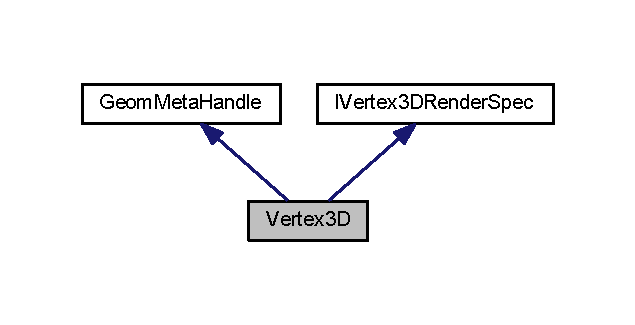
\includegraphics[width=305pt]{class_vertex3_d__inherit__graph}
\end{center}
\end{figure}


Collaboration diagram for Vertex3\-D\-:\nopagebreak
\begin{figure}[H]
\begin{center}
\leavevmode
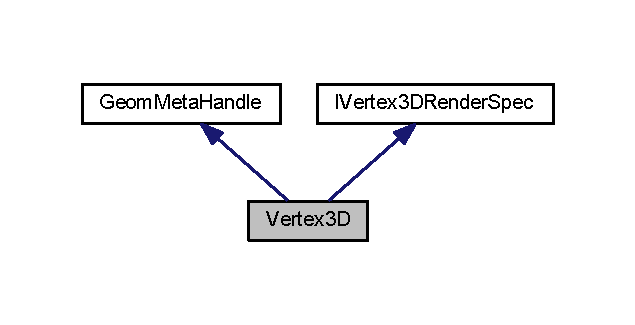
\includegraphics[width=305pt]{class_vertex3_d__coll__graph}
\end{center}
\end{figure}
\subsection*{Public Member Functions}
\begin{DoxyCompactItemize}
\item 
\hypertarget{class_vertex3_d_a41dee42f7502bdc4b04be44a4bf4bdbc}{\hyperlink{class_vertex3_d_a41dee42f7502bdc4b04be44a4bf4bdbc}{Vertex3\-D} ()}\label{class_vertex3_d_a41dee42f7502bdc4b04be44a4bf4bdbc}

\begin{DoxyCompactList}\small\item\em Constructor. Initialises position and I\-D to zero. \end{DoxyCompactList}\item 
\hyperlink{class_vertex3_d_a81b68cf7e781884ed457034bd5b63612}{Vertex3\-D} (const float x, const float y, const float z)
\begin{DoxyCompactList}\small\item\em Constructor specifying vertex position. \end{DoxyCompactList}\item 
\hyperlink{class_vertex3_d_a11ea685931b50972afb2ffda7bfaa984}{Vertex3\-D} (const Q\-Vector3\-D vec)
\begin{DoxyCompactList}\small\item\em Constructor specifying vertex position. \end{DoxyCompactList}\item 
Q\-Vector3\-D \hyperlink{class_vertex3_d_aefb3922097ae3d982370671c2c83fe1d}{get\-Position} () const 
\begin{DoxyCompactList}\small\item\em Gets the vertex's position local to its parent geometry object. \end{DoxyCompactList}\item 
Q\-Color \hyperlink{class_vertex3_d_a2bdd677bf1eb764a7dfa967aa7d2660b}{get\-Colour} () const 
\begin{DoxyCompactList}\small\item\em Gets the vertex's render colour. \end{DoxyCompactList}\item 
Q\-Vector3\-D \hyperlink{class_vertex3_d_a02604a70c43c9ef567684174e8406959}{get\-Normal} () const 
\begin{DoxyCompactList}\small\item\em Gets this vertex's normal. \end{DoxyCompactList}\item 
float \hyperlink{class_vertex3_d_ad22bd676ad371c1a3ba6e987e0704733}{get\-Tex\-Coord\-X} () const 
\begin{DoxyCompactList}\small\item\em Gets this vertex's X texture co-\/ordinate. \end{DoxyCompactList}\item 
float \hyperlink{class_vertex3_d_a3b6eab91dea0d4eb0c53d6c414bda232}{get\-Tex\-Coord\-Y} () const 
\begin{DoxyCompactList}\small\item\em Gets this vertex's Y texture co-\/ordinate. \end{DoxyCompactList}\item 
\hyperlink{vertex_8h_a2e2e1374aac5842116c8683f3b06e99f}{V\-B\-O\-\_\-\-O\-F\-F\-S\-E\-T} \hyperlink{class_vertex3_d_a04dca81ead78614468f7028913a2a582}{get\-V\-B\-O\-Offset} () const 
\begin{DoxyCompactList}\small\item\em Gets this vertex's V\-B\-O offset from the beginning of the parent solid. This offset it not valid if the parent solid is N\-U\-L\-L\-H\-N\-D. \end{DoxyCompactList}\item 
\hyperlink{vertex_8h_a72202e57358ed73cd212e9a2eaf39aeb}{G\-E\-O\-M\-H\-A\-N\-D\-L\-E} \hyperlink{class_vertex3_d_a77b0e7b96b5ec626d56ea32963111c37}{get\-Parent\-Solid} () const 
\begin{DoxyCompactList}\small\item\em Gets the handle of this vertex's parent solid. \end{DoxyCompactList}\item 
\hyperlink{vertex_8h_a72202e57358ed73cd212e9a2eaf39aeb}{G\-E\-O\-M\-H\-A\-N\-D\-L\-E} \hyperlink{class_vertex3_d_acd4bdbddebb5090650cd31883280175e}{get\-Handle} () const 
\begin{DoxyCompactList}\small\item\em Returns this vertex's handle, which is unique within its parent solid. \end{DoxyCompactList}\item 
void \hyperlink{class_vertex3_d_a0727071117d99f6a5f5227b54d41a7cf}{set\-Position} (const float x, const float y, const float z)
\begin{DoxyCompactList}\small\item\em Sets the vertex's position. \end{DoxyCompactList}\item 
void \hyperlink{class_vertex3_d_a62274f5655891dc5dfe979bc2c57ded6}{set\-Position} (const Q\-Vector3\-D pos)
\begin{DoxyCompactList}\small\item\em Sets the vertex's position. \end{DoxyCompactList}\item 
void \hyperlink{class_vertex3_d_ac922ca7c683657d60be4147d17d2d74e}{set\-Colour} (const Q\-Color colour)
\begin{DoxyCompactList}\small\item\em Sets the vertex's render colour. \end{DoxyCompactList}\item 
void \hyperlink{class_vertex3_d_a512576966b5a70493353df7f3571e727}{set\-Normal} (const Q\-Vector3\-D normal)
\begin{DoxyCompactList}\small\item\em Sets this vertex's normal. \end{DoxyCompactList}\item 
void \hyperlink{class_vertex3_d_a8fba559b69d9ba907d962c7154321854}{set\-Tex\-Coord\-X} (const float coord)
\begin{DoxyCompactList}\small\item\em Sets this vertex's X texture co-\/ordinate. \end{DoxyCompactList}\item 
void \hyperlink{class_vertex3_d_a72cc82c3b015c4aabd5a2223933655b5}{set\-Tex\-Coord\-Y} (const float coord)
\begin{DoxyCompactList}\small\item\em Sets this vertex's Y texture co-\/ordinate. \end{DoxyCompactList}\item 
void \hyperlink{class_vertex3_d_a8201535f83d869bb1421e7d36962624a}{set\-V\-B\-O\-Offset} (const \hyperlink{vertex_8h_a2e2e1374aac5842116c8683f3b06e99f}{V\-B\-O\-\_\-\-O\-F\-F\-S\-E\-T} offset)
\begin{DoxyCompactList}\small\item\em Sets this vertex's V\-B\-O offset. \end{DoxyCompactList}\item 
void \hyperlink{class_vertex3_d_aec0f45cdc6b03ec560fd4c352c6bd694}{set\-Parent\-Solid} (const \hyperlink{vertex_8h_a72202e57358ed73cd212e9a2eaf39aeb}{G\-E\-O\-M\-H\-A\-N\-D\-L\-E} handle)
\begin{DoxyCompactList}\small\item\em Sets this vertex's parent solid handle. \end{DoxyCompactList}\item 
void \hyperlink{class_vertex3_d_a53670951cc49d1b5ae9d03d08a11d581}{set\-Handle} (const \hyperlink{vertex_8h_a72202e57358ed73cd212e9a2eaf39aeb}{G\-E\-O\-M\-H\-A\-N\-D\-L\-E} handle)
\begin{DoxyCompactList}\small\item\em Sets this vertex's handle. \end{DoxyCompactList}\item 
virtual void \hyperlink{class_vertex3_d_a1d95bf448d6cf90c2ba78ab22167b806}{V3\-R\-S\-\_\-\-Position} (float position\mbox{[}$\,$\mbox{]})
\begin{DoxyCompactList}\small\item\em Fills an array with the position values for this vertex. \end{DoxyCompactList}\item 
virtual void \hyperlink{class_vertex3_d_a40126d514f76cfef6ebf2855380338e1}{V3\-R\-S\-\_\-\-Colour} (unsigned char colour\mbox{[}$\,$\mbox{]})
\begin{DoxyCompactList}\small\item\em Fills an array with the colour values for this vertex. \end{DoxyCompactList}\item 
virtual void \hyperlink{class_vertex3_d_aea2d1d899ec54fc166fd04baeee64a91}{V3\-R\-S\-\_\-\-Texture\-\_\-\-Coords} (float coords\mbox{[}$\,$\mbox{]})
\begin{DoxyCompactList}\small\item\em Fills an array with the texture co-\/ordinate values for this vertex. \end{DoxyCompactList}\item 
virtual unsigned long \hyperlink{class_vertex3_d_a13a922fd8180591636c1daf4687cc205}{V3\-R\-S\-\_\-\-Offset} ()
\begin{DoxyCompactList}\small\item\em Returns the offset of this vertex from the beginning of the V\-B\-O, in V3\-R\-S\-\_\-\-T\-O\-T\-A\-L\-\_\-\-D\-A\-T\-A\-\_\-\-T\-R\-A\-N\-S\-F\-E\-R strides. \end{DoxyCompactList}\end{DoxyCompactItemize}
\subsection*{Additional Inherited Members}


\subsection{Detailed Description}
Defines a vertex in 3\-D space. 

The vertex contains a V\-B\-O offset which, when combined with the parent solid's offset, defines where in the V\-B\-O this vertex's render data is found. The vertex also contains colour information and texture co-\/ordinates. Normals are not stored per vertex as when faces are rendered, the face's stored normal is used to calculate the shading required. 

\subsection{Constructor \& Destructor Documentation}
\hypertarget{class_vertex3_d_a81b68cf7e781884ed457034bd5b63612}{\index{Vertex3\-D@{Vertex3\-D}!Vertex3\-D@{Vertex3\-D}}
\index{Vertex3\-D@{Vertex3\-D}!Vertex3D@{Vertex3\-D}}
\subsubsection[{Vertex3\-D}]{\setlength{\rightskip}{0pt plus 5cm}Vertex3\-D\-::\-Vertex3\-D (
\begin{DoxyParamCaption}
\item[{const float}]{x, }
\item[{const float}]{y, }
\item[{const float}]{z}
\end{DoxyParamCaption}
)\hspace{0.3cm}{\ttfamily [inline]}}}\label{class_vertex3_d_a81b68cf7e781884ed457034bd5b63612}


Constructor specifying vertex position. 


\begin{DoxyParams}{Parameters}
{\em x} & X position. \\
\hline
{\em y} & Y position. \\
\hline
{\em z} & Z position. \\
\hline
\end{DoxyParams}
\hypertarget{class_vertex3_d_a11ea685931b50972afb2ffda7bfaa984}{\index{Vertex3\-D@{Vertex3\-D}!Vertex3\-D@{Vertex3\-D}}
\index{Vertex3\-D@{Vertex3\-D}!Vertex3D@{Vertex3\-D}}
\subsubsection[{Vertex3\-D}]{\setlength{\rightskip}{0pt plus 5cm}Vertex3\-D\-::\-Vertex3\-D (
\begin{DoxyParamCaption}
\item[{const Q\-Vector3\-D}]{vec}
\end{DoxyParamCaption}
)\hspace{0.3cm}{\ttfamily [inline]}}}\label{class_vertex3_d_a11ea685931b50972afb2ffda7bfaa984}


Constructor specifying vertex position. 


\begin{DoxyParams}{Parameters}
{\em vec} & Vector representing position. \\
\hline
\end{DoxyParams}


\subsection{Member Function Documentation}
\hypertarget{class_vertex3_d_a2bdd677bf1eb764a7dfa967aa7d2660b}{\index{Vertex3\-D@{Vertex3\-D}!get\-Colour@{get\-Colour}}
\index{get\-Colour@{get\-Colour}!Vertex3D@{Vertex3\-D}}
\subsubsection[{get\-Colour}]{\setlength{\rightskip}{0pt plus 5cm}Q\-Color Vertex3\-D\-::get\-Colour (
\begin{DoxyParamCaption}
{}
\end{DoxyParamCaption}
) const\hspace{0.3cm}{\ttfamily [inline]}}}\label{class_vertex3_d_a2bdd677bf1eb764a7dfa967aa7d2660b}


Gets the vertex's render colour. 

\begin{DoxyReturn}{Returns}
Render colour. 
\end{DoxyReturn}
\hypertarget{class_vertex3_d_acd4bdbddebb5090650cd31883280175e}{\index{Vertex3\-D@{Vertex3\-D}!get\-Handle@{get\-Handle}}
\index{get\-Handle@{get\-Handle}!Vertex3D@{Vertex3\-D}}
\subsubsection[{get\-Handle}]{\setlength{\rightskip}{0pt plus 5cm}{\bf G\-E\-O\-M\-H\-A\-N\-D\-L\-E} Vertex3\-D\-::get\-Handle (
\begin{DoxyParamCaption}
{}
\end{DoxyParamCaption}
) const\hspace{0.3cm}{\ttfamily [inline]}}}\label{class_vertex3_d_acd4bdbddebb5090650cd31883280175e}


Returns this vertex's handle, which is unique within its parent solid. 

\begin{DoxyReturn}{Returns}
This vertex's handle. 
\end{DoxyReturn}
\hypertarget{class_vertex3_d_a02604a70c43c9ef567684174e8406959}{\index{Vertex3\-D@{Vertex3\-D}!get\-Normal@{get\-Normal}}
\index{get\-Normal@{get\-Normal}!Vertex3D@{Vertex3\-D}}
\subsubsection[{get\-Normal}]{\setlength{\rightskip}{0pt plus 5cm}Q\-Vector3\-D Vertex3\-D\-::get\-Normal (
\begin{DoxyParamCaption}
{}
\end{DoxyParamCaption}
) const\hspace{0.3cm}{\ttfamily [inline]}}}\label{class_vertex3_d_a02604a70c43c9ef567684174e8406959}


Gets this vertex's normal. 

\begin{DoxyReturn}{Returns}
Normal vector. 
\end{DoxyReturn}
\hypertarget{class_vertex3_d_a77b0e7b96b5ec626d56ea32963111c37}{\index{Vertex3\-D@{Vertex3\-D}!get\-Parent\-Solid@{get\-Parent\-Solid}}
\index{get\-Parent\-Solid@{get\-Parent\-Solid}!Vertex3D@{Vertex3\-D}}
\subsubsection[{get\-Parent\-Solid}]{\setlength{\rightskip}{0pt plus 5cm}{\bf G\-E\-O\-M\-H\-A\-N\-D\-L\-E} Vertex3\-D\-::get\-Parent\-Solid (
\begin{DoxyParamCaption}
{}
\end{DoxyParamCaption}
) const\hspace{0.3cm}{\ttfamily [inline]}}}\label{class_vertex3_d_a77b0e7b96b5ec626d56ea32963111c37}


Gets the handle of this vertex's parent solid. 

\begin{DoxyReturn}{Returns}
Parent solid's handle, or N\-U\-L\-L\-H\-N\-D if no parent solid exists. 
\end{DoxyReturn}
\hypertarget{class_vertex3_d_aefb3922097ae3d982370671c2c83fe1d}{\index{Vertex3\-D@{Vertex3\-D}!get\-Position@{get\-Position}}
\index{get\-Position@{get\-Position}!Vertex3D@{Vertex3\-D}}
\subsubsection[{get\-Position}]{\setlength{\rightskip}{0pt plus 5cm}Q\-Vector3\-D Vertex3\-D\-::get\-Position (
\begin{DoxyParamCaption}
{}
\end{DoxyParamCaption}
) const\hspace{0.3cm}{\ttfamily [inline]}}}\label{class_vertex3_d_aefb3922097ae3d982370671c2c83fe1d}


Gets the vertex's position local to its parent geometry object. 

\begin{DoxyReturn}{Returns}
Vector representing position. 
\end{DoxyReturn}
\hypertarget{class_vertex3_d_ad22bd676ad371c1a3ba6e987e0704733}{\index{Vertex3\-D@{Vertex3\-D}!get\-Tex\-Coord\-X@{get\-Tex\-Coord\-X}}
\index{get\-Tex\-Coord\-X@{get\-Tex\-Coord\-X}!Vertex3D@{Vertex3\-D}}
\subsubsection[{get\-Tex\-Coord\-X}]{\setlength{\rightskip}{0pt plus 5cm}float Vertex3\-D\-::get\-Tex\-Coord\-X (
\begin{DoxyParamCaption}
{}
\end{DoxyParamCaption}
) const\hspace{0.3cm}{\ttfamily [inline]}}}\label{class_vertex3_d_ad22bd676ad371c1a3ba6e987e0704733}


Gets this vertex's X texture co-\/ordinate. 

\begin{DoxyReturn}{Returns}
X co-\/ordinate. 
\end{DoxyReturn}
\hypertarget{class_vertex3_d_a3b6eab91dea0d4eb0c53d6c414bda232}{\index{Vertex3\-D@{Vertex3\-D}!get\-Tex\-Coord\-Y@{get\-Tex\-Coord\-Y}}
\index{get\-Tex\-Coord\-Y@{get\-Tex\-Coord\-Y}!Vertex3D@{Vertex3\-D}}
\subsubsection[{get\-Tex\-Coord\-Y}]{\setlength{\rightskip}{0pt plus 5cm}float Vertex3\-D\-::get\-Tex\-Coord\-Y (
\begin{DoxyParamCaption}
{}
\end{DoxyParamCaption}
) const\hspace{0.3cm}{\ttfamily [inline]}}}\label{class_vertex3_d_a3b6eab91dea0d4eb0c53d6c414bda232}


Gets this vertex's Y texture co-\/ordinate. 

\begin{DoxyReturn}{Returns}
Y co-\/ordinate. 
\end{DoxyReturn}
\hypertarget{class_vertex3_d_a04dca81ead78614468f7028913a2a582}{\index{Vertex3\-D@{Vertex3\-D}!get\-V\-B\-O\-Offset@{get\-V\-B\-O\-Offset}}
\index{get\-V\-B\-O\-Offset@{get\-V\-B\-O\-Offset}!Vertex3D@{Vertex3\-D}}
\subsubsection[{get\-V\-B\-O\-Offset}]{\setlength{\rightskip}{0pt plus 5cm}{\bf V\-B\-O\-\_\-\-O\-F\-F\-S\-E\-T} Vertex3\-D\-::get\-V\-B\-O\-Offset (
\begin{DoxyParamCaption}
{}
\end{DoxyParamCaption}
) const\hspace{0.3cm}{\ttfamily [inline]}}}\label{class_vertex3_d_a04dca81ead78614468f7028913a2a582}


Gets this vertex's V\-B\-O offset from the beginning of the parent solid. This offset it not valid if the parent solid is N\-U\-L\-L\-H\-N\-D. 

\begin{DoxyReturn}{Returns}
Vertex's V\-B\-O offset. 
\end{DoxyReturn}
\hypertarget{class_vertex3_d_ac922ca7c683657d60be4147d17d2d74e}{\index{Vertex3\-D@{Vertex3\-D}!set\-Colour@{set\-Colour}}
\index{set\-Colour@{set\-Colour}!Vertex3D@{Vertex3\-D}}
\subsubsection[{set\-Colour}]{\setlength{\rightskip}{0pt plus 5cm}void Vertex3\-D\-::set\-Colour (
\begin{DoxyParamCaption}
\item[{const Q\-Color}]{colour}
\end{DoxyParamCaption}
)\hspace{0.3cm}{\ttfamily [inline]}}}\label{class_vertex3_d_ac922ca7c683657d60be4147d17d2d74e}


Sets the vertex's render colour. 


\begin{DoxyParams}{Parameters}
{\em colour} & Colour to set. \\
\hline
\end{DoxyParams}
\hypertarget{class_vertex3_d_a53670951cc49d1b5ae9d03d08a11d581}{\index{Vertex3\-D@{Vertex3\-D}!set\-Handle@{set\-Handle}}
\index{set\-Handle@{set\-Handle}!Vertex3D@{Vertex3\-D}}
\subsubsection[{set\-Handle}]{\setlength{\rightskip}{0pt plus 5cm}void Vertex3\-D\-::set\-Handle (
\begin{DoxyParamCaption}
\item[{const {\bf G\-E\-O\-M\-H\-A\-N\-D\-L\-E}}]{handle}
\end{DoxyParamCaption}
)\hspace{0.3cm}{\ttfamily [inline]}}}\label{class_vertex3_d_a53670951cc49d1b5ae9d03d08a11d581}


Sets this vertex's handle. 


\begin{DoxyParams}{Parameters}
{\em handle} & Handle to set. \\
\hline
\end{DoxyParams}
\hypertarget{class_vertex3_d_a512576966b5a70493353df7f3571e727}{\index{Vertex3\-D@{Vertex3\-D}!set\-Normal@{set\-Normal}}
\index{set\-Normal@{set\-Normal}!Vertex3D@{Vertex3\-D}}
\subsubsection[{set\-Normal}]{\setlength{\rightskip}{0pt plus 5cm}void Vertex3\-D\-::set\-Normal (
\begin{DoxyParamCaption}
\item[{const Q\-Vector3\-D}]{normal}
\end{DoxyParamCaption}
)\hspace{0.3cm}{\ttfamily [inline]}}}\label{class_vertex3_d_a512576966b5a70493353df7f3571e727}


Sets this vertex's normal. 


\begin{DoxyParams}{Parameters}
{\em normal} & Normal to set. \\
\hline
\end{DoxyParams}
\hypertarget{class_vertex3_d_aec0f45cdc6b03ec560fd4c352c6bd694}{\index{Vertex3\-D@{Vertex3\-D}!set\-Parent\-Solid@{set\-Parent\-Solid}}
\index{set\-Parent\-Solid@{set\-Parent\-Solid}!Vertex3D@{Vertex3\-D}}
\subsubsection[{set\-Parent\-Solid}]{\setlength{\rightskip}{0pt plus 5cm}void Vertex3\-D\-::set\-Parent\-Solid (
\begin{DoxyParamCaption}
\item[{const {\bf G\-E\-O\-M\-H\-A\-N\-D\-L\-E}}]{handle}
\end{DoxyParamCaption}
)\hspace{0.3cm}{\ttfamily [inline]}}}\label{class_vertex3_d_aec0f45cdc6b03ec560fd4c352c6bd694}


Sets this vertex's parent solid handle. 


\begin{DoxyParams}{Parameters}
{\em handle} & Handle to set. \\
\hline
\end{DoxyParams}
\hypertarget{class_vertex3_d_a0727071117d99f6a5f5227b54d41a7cf}{\index{Vertex3\-D@{Vertex3\-D}!set\-Position@{set\-Position}}
\index{set\-Position@{set\-Position}!Vertex3D@{Vertex3\-D}}
\subsubsection[{set\-Position}]{\setlength{\rightskip}{0pt plus 5cm}void Vertex3\-D\-::set\-Position (
\begin{DoxyParamCaption}
\item[{const float}]{x, }
\item[{const float}]{y, }
\item[{const float}]{z}
\end{DoxyParamCaption}
)\hspace{0.3cm}{\ttfamily [inline]}}}\label{class_vertex3_d_a0727071117d99f6a5f5227b54d41a7cf}


Sets the vertex's position. 


\begin{DoxyParams}{Parameters}
{\em x} & X position. \\
\hline
{\em y} & Y position. \\
\hline
{\em z} & Z position. \\
\hline
\end{DoxyParams}
\hypertarget{class_vertex3_d_a62274f5655891dc5dfe979bc2c57ded6}{\index{Vertex3\-D@{Vertex3\-D}!set\-Position@{set\-Position}}
\index{set\-Position@{set\-Position}!Vertex3D@{Vertex3\-D}}
\subsubsection[{set\-Position}]{\setlength{\rightskip}{0pt plus 5cm}void Vertex3\-D\-::set\-Position (
\begin{DoxyParamCaption}
\item[{const Q\-Vector3\-D}]{pos}
\end{DoxyParamCaption}
)\hspace{0.3cm}{\ttfamily [inline]}}}\label{class_vertex3_d_a62274f5655891dc5dfe979bc2c57ded6}


Sets the vertex's position. 


\begin{DoxyParams}{Parameters}
{\em pos} & Vector representing position. \\
\hline
\end{DoxyParams}
\hypertarget{class_vertex3_d_a8fba559b69d9ba907d962c7154321854}{\index{Vertex3\-D@{Vertex3\-D}!set\-Tex\-Coord\-X@{set\-Tex\-Coord\-X}}
\index{set\-Tex\-Coord\-X@{set\-Tex\-Coord\-X}!Vertex3D@{Vertex3\-D}}
\subsubsection[{set\-Tex\-Coord\-X}]{\setlength{\rightskip}{0pt plus 5cm}void Vertex3\-D\-::set\-Tex\-Coord\-X (
\begin{DoxyParamCaption}
\item[{const float}]{coord}
\end{DoxyParamCaption}
)\hspace{0.3cm}{\ttfamily [inline]}}}\label{class_vertex3_d_a8fba559b69d9ba907d962c7154321854}


Sets this vertex's X texture co-\/ordinate. 


\begin{DoxyParams}{Parameters}
{\em coord} & Co-\/ord to set. \\
\hline
\end{DoxyParams}
\hypertarget{class_vertex3_d_a72cc82c3b015c4aabd5a2223933655b5}{\index{Vertex3\-D@{Vertex3\-D}!set\-Tex\-Coord\-Y@{set\-Tex\-Coord\-Y}}
\index{set\-Tex\-Coord\-Y@{set\-Tex\-Coord\-Y}!Vertex3D@{Vertex3\-D}}
\subsubsection[{set\-Tex\-Coord\-Y}]{\setlength{\rightskip}{0pt plus 5cm}void Vertex3\-D\-::set\-Tex\-Coord\-Y (
\begin{DoxyParamCaption}
\item[{const float}]{coord}
\end{DoxyParamCaption}
)\hspace{0.3cm}{\ttfamily [inline]}}}\label{class_vertex3_d_a72cc82c3b015c4aabd5a2223933655b5}


Sets this vertex's Y texture co-\/ordinate. 


\begin{DoxyParams}{Parameters}
{\em coord} & Co-\/ord to set. \\
\hline
\end{DoxyParams}
\hypertarget{class_vertex3_d_a8201535f83d869bb1421e7d36962624a}{\index{Vertex3\-D@{Vertex3\-D}!set\-V\-B\-O\-Offset@{set\-V\-B\-O\-Offset}}
\index{set\-V\-B\-O\-Offset@{set\-V\-B\-O\-Offset}!Vertex3D@{Vertex3\-D}}
\subsubsection[{set\-V\-B\-O\-Offset}]{\setlength{\rightskip}{0pt plus 5cm}void Vertex3\-D\-::set\-V\-B\-O\-Offset (
\begin{DoxyParamCaption}
\item[{const {\bf V\-B\-O\-\_\-\-O\-F\-F\-S\-E\-T}}]{offset}
\end{DoxyParamCaption}
)\hspace{0.3cm}{\ttfamily [inline]}}}\label{class_vertex3_d_a8201535f83d869bb1421e7d36962624a}


Sets this vertex's V\-B\-O offset. 


\begin{DoxyParams}{Parameters}
{\em offset} & Offset to set. \\
\hline
\end{DoxyParams}
\hypertarget{class_vertex3_d_a40126d514f76cfef6ebf2855380338e1}{\index{Vertex3\-D@{Vertex3\-D}!V3\-R\-S\-\_\-\-Colour@{V3\-R\-S\-\_\-\-Colour}}
\index{V3\-R\-S\-\_\-\-Colour@{V3\-R\-S\-\_\-\-Colour}!Vertex3D@{Vertex3\-D}}
\subsubsection[{V3\-R\-S\-\_\-\-Colour}]{\setlength{\rightskip}{0pt plus 5cm}virtual void Vertex3\-D\-::\-V3\-R\-S\-\_\-\-Colour (
\begin{DoxyParamCaption}
\item[{unsigned char}]{colour\mbox{[}$\,$\mbox{]}}
\end{DoxyParamCaption}
)\hspace{0.3cm}{\ttfamily [inline]}, {\ttfamily [virtual]}}}\label{class_vertex3_d_a40126d514f76cfef6ebf2855380338e1}


Fills an array with the colour values for this vertex. 


\begin{DoxyParams}{Parameters}
{\em colour} & Colour values. Format is R\-G\-B\-A, range 0.\-0 -\/ 1.\-0. \\
\hline
\end{DoxyParams}
\hypertarget{class_vertex3_d_a13a922fd8180591636c1daf4687cc205}{\index{Vertex3\-D@{Vertex3\-D}!V3\-R\-S\-\_\-\-Offset@{V3\-R\-S\-\_\-\-Offset}}
\index{V3\-R\-S\-\_\-\-Offset@{V3\-R\-S\-\_\-\-Offset}!Vertex3D@{Vertex3\-D}}
\subsubsection[{V3\-R\-S\-\_\-\-Offset}]{\setlength{\rightskip}{0pt plus 5cm}virtual unsigned long Vertex3\-D\-::\-V3\-R\-S\-\_\-\-Offset (
\begin{DoxyParamCaption}
{}
\end{DoxyParamCaption}
)\hspace{0.3cm}{\ttfamily [inline]}, {\ttfamily [virtual]}}}\label{class_vertex3_d_a13a922fd8180591636c1daf4687cc205}


Returns the offset of this vertex from the beginning of the V\-B\-O, in V3\-R\-S\-\_\-\-T\-O\-T\-A\-L\-\_\-\-D\-A\-T\-A\-\_\-\-T\-R\-A\-N\-S\-F\-E\-R strides. 

\begin{DoxyReturn}{Returns}
Offset for this vertex. 
\end{DoxyReturn}


Implements \hyperlink{class_i_vertex3_d_render_spec_a891d736d3d414de333398975f34bbae7}{I\-Vertex3\-D\-Render\-Spec}.

\hypertarget{class_vertex3_d_a1d95bf448d6cf90c2ba78ab22167b806}{\index{Vertex3\-D@{Vertex3\-D}!V3\-R\-S\-\_\-\-Position@{V3\-R\-S\-\_\-\-Position}}
\index{V3\-R\-S\-\_\-\-Position@{V3\-R\-S\-\_\-\-Position}!Vertex3D@{Vertex3\-D}}
\subsubsection[{V3\-R\-S\-\_\-\-Position}]{\setlength{\rightskip}{0pt plus 5cm}virtual void Vertex3\-D\-::\-V3\-R\-S\-\_\-\-Position (
\begin{DoxyParamCaption}
\item[{float}]{position\mbox{[}$\,$\mbox{]}}
\end{DoxyParamCaption}
)\hspace{0.3cm}{\ttfamily [inline]}, {\ttfamily [virtual]}}}\label{class_vertex3_d_a1d95bf448d6cf90c2ba78ab22167b806}


Fills an array with the position values for this vertex. 


\begin{DoxyParams}{Parameters}
{\em position} & Array to fill. Format is X\-Y\-Z. \\
\hline
\end{DoxyParams}
\hypertarget{class_vertex3_d_aea2d1d899ec54fc166fd04baeee64a91}{\index{Vertex3\-D@{Vertex3\-D}!V3\-R\-S\-\_\-\-Texture\-\_\-\-Coords@{V3\-R\-S\-\_\-\-Texture\-\_\-\-Coords}}
\index{V3\-R\-S\-\_\-\-Texture\-\_\-\-Coords@{V3\-R\-S\-\_\-\-Texture\-\_\-\-Coords}!Vertex3D@{Vertex3\-D}}
\subsubsection[{V3\-R\-S\-\_\-\-Texture\-\_\-\-Coords}]{\setlength{\rightskip}{0pt plus 5cm}virtual void Vertex3\-D\-::\-V3\-R\-S\-\_\-\-Texture\-\_\-\-Coords (
\begin{DoxyParamCaption}
\item[{float}]{coords\mbox{[}$\,$\mbox{]}}
\end{DoxyParamCaption}
)\hspace{0.3cm}{\ttfamily [inline]}, {\ttfamily [virtual]}}}\label{class_vertex3_d_aea2d1d899ec54fc166fd04baeee64a91}


Fills an array with the texture co-\/ordinate values for this vertex. 


\begin{DoxyParams}{Parameters}
{\em coords} & Array to fill. Format is X\-Y. \\
\hline
\end{DoxyParams}


The documentation for this class was generated from the following file\-:\begin{DoxyCompactItemize}
\item 
app/\hyperlink{vertex_8h}{vertex.\-h}\end{DoxyCompactItemize}

\chapter{File Documentation}
\hypertarget{baseproperty_8h}{\section{app/baseproperty.h File Reference}
\label{baseproperty_8h}\index{app/baseproperty.\-h@{app/baseproperty.\-h}}
}


Defines the property base class and interfaces.  


{\ttfamily \#include $<$Q\-Object$>$}\\*
{\ttfamily \#include $<$Q\-Pair$>$}\\*
Include dependency graph for baseproperty.\-h\-:
\nopagebreak
\begin{figure}[H]
\begin{center}
\leavevmode
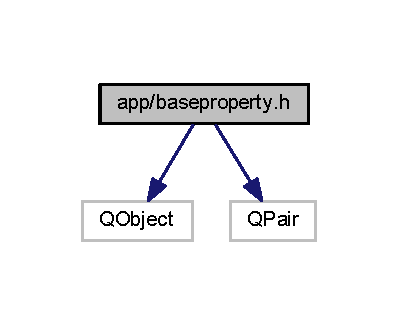
\includegraphics[width=191pt]{baseproperty_8h__incl}
\end{center}
\end{figure}
This graph shows which files directly or indirectly include this file\-:
\nopagebreak
\begin{figure}[H]
\begin{center}
\leavevmode
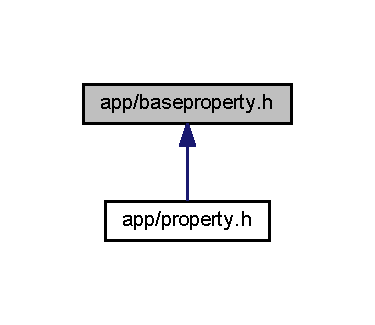
\includegraphics[width=180pt]{baseproperty_8h__dep__incl}
\end{center}
\end{figure}
\subsection*{Classes}
\begin{DoxyCompactItemize}
\item 
class \hyperlink{class_i_base_property}{I\-Base\-Property}
\begin{DoxyCompactList}\small\item\em Base property interface. \end{DoxyCompactList}\item 
class \hyperlink{class_w_base_property}{W\-Base\-Property}
\begin{DoxyCompactList}\small\item\em Base property interface wrapper. \end{DoxyCompactList}\item 
class \hyperlink{class_base_property}{Base\-Property}
\begin{DoxyCompactList}\small\item\em Base property class. \end{DoxyCompactList}\item 
class \hyperlink{class_i_property_variant}{I\-Property\-Variant}
\begin{DoxyCompactList}\small\item\em Interface implemented by \hyperlink{class_property_variant}{Property\-Variant}. \end{DoxyCompactList}\item 
class \hyperlink{class_w_property_variant}{W\-Property\-Variant}
\begin{DoxyCompactList}\small\item\em \hyperlink{class_property_variant}{Property\-Variant} interface wrapper. \end{DoxyCompactList}\item 
class \hyperlink{class_property_variant}{Property\-Variant}
\begin{DoxyCompactList}\small\item\em Allows fetching of subclassed properties from a list of \hyperlink{class_base_property}{Base\-Property} pointers. \end{DoxyCompactList}\end{DoxyCompactItemize}
\subsection*{Macros}
\begin{DoxyCompactItemize}
\item 
\hypertarget{group___property_classes_gade3d7799947a250392e929b65d46f1d8}{\#define \hyperlink{group___property_classes_gade3d7799947a250392e929b65d46f1d8}{I\-Base\-Property\-\_\-iid}~\char`\"{}Crowbar.\-Interfaces.\-I\-Base\-Property\char`\"{}}\label{group___property_classes_gade3d7799947a250392e929b65d46f1d8}

\begin{DoxyCompactList}\small\item\em Unique I\-D for \hyperlink{class_i_base_property}{I\-Base\-Property} interface. \end{DoxyCompactList}\item 
\hypertarget{group___property_classes_ga2f1443d00c2aa858e3321a7cdc6f5e4a}{\#define \hyperlink{group___property_classes_ga2f1443d00c2aa858e3321a7cdc6f5e4a}{I\-Property\-Variant\-\_\-iid}~\char`\"{}Crowbar.\-Interfaces.\-I\-Property\-Variant\char`\"{}}\label{group___property_classes_ga2f1443d00c2aa858e3321a7cdc6f5e4a}

\begin{DoxyCompactList}\small\item\em Unique I\-D for \hyperlink{class_i_property_variant}{I\-Property\-Variant} interface. \end{DoxyCompactList}\item 
\#define \hyperlink{group___property_classes_ga8621ccbce057779b93b54f2f06440126}{D\-E\-C\-L\-A\-R\-E\-\_\-\-V\-A\-R\-I\-A\-N\-T\-\_\-\-G\-E\-T\-M\-E\-T\-H\-O\-D}(\-\_\-methodname, \-\_\-type)~\-\_\-type \-\_\-methodname() const \{ return m\-\_\-\#\#\-\_\-type; \}
\begin{DoxyCompactList}\small\item\em M\-A\-C\-R\-O M\-E\-T\-H\-O\-D\-: Gets variant \-\_\-type value. \end{DoxyCompactList}\item 
\#define \hyperlink{group___property_classes_gab10c17d63104a3b2b6e8c26baeb1548b}{D\-E\-C\-L\-A\-R\-E\-\_\-\-V\-A\-R\-I\-A\-N\-T\-\_\-\-S\-E\-T\-M\-E\-T\-H\-O\-D}(\-\_\-methodname, \-\_\-type)~void \-\_\-methodname(\-\_\-type value) \{ m\-\_\-\#\#\-\_\-type = value; \}
\begin{DoxyCompactList}\small\item\em M\-A\-C\-R\-O M\-E\-T\-H\-O\-D\-: Sets variant \-\_\-type value. \end{DoxyCompactList}\item 
\#define \hyperlink{group___property_classes_ga6ceaa3b2a99aaa90a1ea66489d2bcc86}{D\-E\-C\-L\-A\-R\-E\-\_\-\-V\-A\-R\-I\-A\-N\-T\-\_\-\-T\-Y\-P\-E}(\-\_\-type)~\-\_\-type m\-\_\-\#\#\-\_\-type;
\begin{DoxyCompactList}\small\item\em M\-A\-C\-R\-O M\-E\-T\-H\-O\-D\-: Declares a member variable of the specified type, to be used with get and set methods. \end{DoxyCompactList}\item 
\#define \hyperlink{group___property_classes_ga336b645c5f84965e75abdf9213c0957e}{C\-L\-E\-A\-N\-\_\-\-V\-A\-R\-I\-A\-N\-T\-\_\-\-T\-Y\-P\-E}(\-\_\-type, \-\_\-value)~m\-\_\-\#\#\-\_\-type = \-\_\-value;
\begin{DoxyCompactList}\small\item\em M\-A\-C\-R\-O M\-E\-T\-H\-O\-D\-: Specifies the safe default value to set a data member to when the variant is cleaned. The type should have been declared with D\-E\-C\-L\-A\-R\-E\-\_\-\-V\-A\-R\-I\-A\-N\-T\-\_\-\-T\-Y\-P\-E. \end{DoxyCompactList}\end{DoxyCompactItemize}
\subsection*{Enumerations}
\begin{DoxyCompactItemize}
\item 
enum \hyperlink{group___property_classes_ga38f1ccddda12c7cb50b868c9f789ee37}{Property\-\_\-t} \{ \\*
\hyperlink{group___property_classes_gga38f1ccddda12c7cb50b868c9f789ee37a14429bef1f04b883474e765ca0c3ae29}{Prop\-\_\-\-None} = -\/1, 
\hyperlink{group___property_classes_gga38f1ccddda12c7cb50b868c9f789ee37a54096075ee9bf1c6f2e44ad7cea76260}{Prop\-\_\-\-String}, 
\hyperlink{group___property_classes_gga38f1ccddda12c7cb50b868c9f789ee37aebb523c385feb37fcde4c6d7073224b7}{Prop\-\_\-\-Int}, 
\hyperlink{group___property_classes_gga38f1ccddda12c7cb50b868c9f789ee37ac42814aa5ea34e3b019db068494eed4d}{Prop\-\_\-\-U\-Int}, 
\\*
\hyperlink{group___property_classes_gga38f1ccddda12c7cb50b868c9f789ee37a48c7c9a2c7bf7b44ae8d4493b5122925}{Prop\-\_\-\-Long}, 
\hyperlink{group___property_classes_gga38f1ccddda12c7cb50b868c9f789ee37a19c6a4ad42555fcc0e2fac1d50fd2035}{Prop\-\_\-\-U\-Long}, 
\hyperlink{group___property_classes_gga38f1ccddda12c7cb50b868c9f789ee37a002f0049641d4e6f52901f023ef44f0c}{Prop\-\_\-\-Float}, 
\hyperlink{group___property_classes_gga38f1ccddda12c7cb50b868c9f789ee37a63a9d61b306c5306a47c5126ebd7200e}{Prop\-\_\-\-Double}, 
\\*
\hyperlink{group___property_classes_gga38f1ccddda12c7cb50b868c9f789ee37a1a1448256ec42f662e39fe120b92073a}{Prop\-\_\-\-Long\-Long}, 
\hyperlink{group___property_classes_gga38f1ccddda12c7cb50b868c9f789ee37aeb9cf79aeea684f28a149fdcd0f593aa}{Prop\-\_\-\-U\-Long\-Long}
 \}
\begin{DoxyCompactList}\small\item\em Property type identifiers. \end{DoxyCompactList}\end{DoxyCompactItemize}


\subsection{Detailed Description}
Defines the property base class and interfaces. The property classes hold a key and a value -\/ these are underlyingly represented as strings and \hyperlink{class_base_property}{Base\-Property} subclasses (defined in \hyperlink{property_8h}{property.\-h}) deal with binding these solidly to interfaces for a specific type. A property's key should endeavour to be unique (it is not defined which property will be selected if two properties have the same key). \par
 \par
 A technical note\-: due to the Qt limitation that only one inheritance of the Q\-Object class is allowed for any derived class (slots requiring an interface inherit from Q\-Object), slots on \hyperlink{class_base_property}{Base\-Property} classes are exposed through a wrapper returned by \hyperlink{class_base_property_a032130dea4bd72ee8dd80dcfa7d5f37a}{Base\-Property\-::slots\-Base()}. Connecting a signal to a slot on this wrapper will call the relevant non-\/slot function on the \hyperlink{class_base_property}{Base\-Property} class. 
\hypertarget{commandlineparser_8h}{\section{app/commandlineparser.h File Reference}
\label{commandlineparser_8h}\index{app/commandlineparser.\-h@{app/commandlineparser.\-h}}
}


Defines the class responsible for parsing command-\/line arguments and setting the relevant settings in response.  


{\ttfamily \#include $<$Q\-Object$>$}\\*
Include dependency graph for commandlineparser.\-h\-:
\nopagebreak
\begin{figure}[H]
\begin{center}
\leavevmode
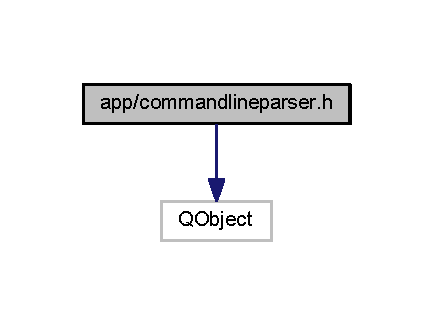
\includegraphics[width=208pt]{commandlineparser_8h__incl}
\end{center}
\end{figure}
\subsection*{Classes}
\begin{DoxyCompactItemize}
\item 
class \hyperlink{class_command_line_parser}{Command\-Line\-Parser}
\begin{DoxyCompactList}\small\item\em Deals with arguments passed to the application on the command-\/line. \end{DoxyCompactList}\end{DoxyCompactItemize}
\subsection*{Macros}
\begin{DoxyCompactItemize}
\item 
\hypertarget{commandlineparser_8h_a28d598b46f4ac21d6aef06c46089f3cb}{\#define \hyperlink{commandlineparser_8h_a28d598b46f4ac21d6aef06c46089f3cb}{C\-L\-A\-\_\-\-D\-E\-B\-U\-G\-G\-I\-N\-G}~\char`\"{}-\/debug\char`\"{}}\label{commandlineparser_8h_a28d598b46f4ac21d6aef06c46089f3cb}

\begin{DoxyCompactList}\small\item\em Command-\/line option string to enable debugging. \end{DoxyCompactList}\item 
\hypertarget{commandlineparser_8h_a886e3ba324ee7244ccb5c79dd2d1cddb}{\#define \hyperlink{commandlineparser_8h_a886e3ba324ee7244ccb5c79dd2d1cddb}{C\-L\-A\-\_\-\-L\-O\-G\-G\-I\-N\-G}~\char`\"{}-\/log\char`\"{}}\label{commandlineparser_8h_a886e3ba324ee7244ccb5c79dd2d1cddb}

\begin{DoxyCompactList}\small\item\em Command-\/line option string to enable logging. \end{DoxyCompactList}\end{DoxyCompactItemize}


\subsection{Detailed Description}
Defines the class responsible for parsing command-\/line arguments and setting the relevant settings in response. 
\hypertarget{edge_8h}{\section{app/edge.h File Reference}
\label{edge_8h}\index{app/edge.\-h@{app/edge.\-h}}
}


Defines an edge which links two vertices.  


{\ttfamily \#include \char`\"{}vertex.\-h\char`\"{}}\\*
Include dependency graph for edge.\-h\-:\nopagebreak
\begin{figure}[H]
\begin{center}
\leavevmode
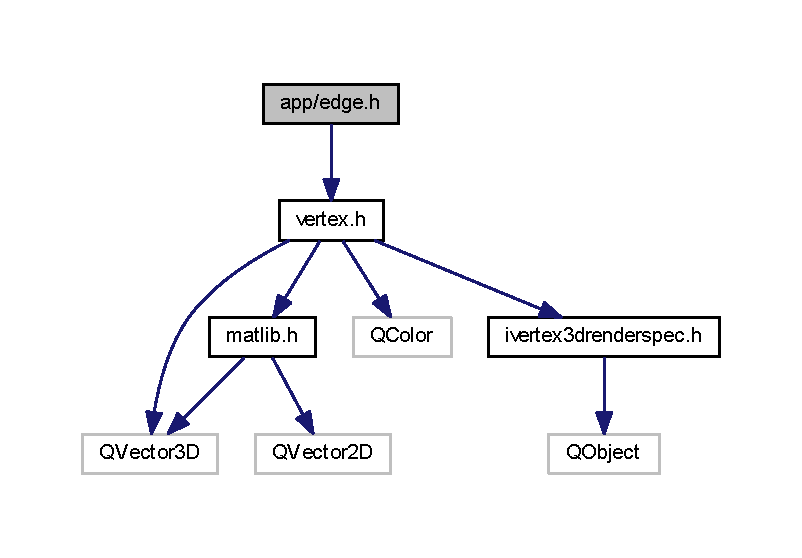
\includegraphics[width=350pt]{edge_8h__incl}
\end{center}
\end{figure}
This graph shows which files directly or indirectly include this file\-:\nopagebreak
\begin{figure}[H]
\begin{center}
\leavevmode
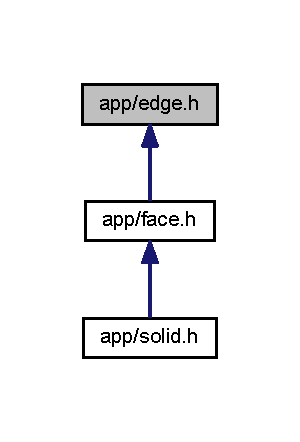
\includegraphics[width=144pt]{edge_8h__dep__incl}
\end{center}
\end{figure}
\subsection*{Classes}
\begin{DoxyCompactItemize}
\item 
class \hyperlink{class_edge3_d}{Edge3\-D}
\begin{DoxyCompactList}\small\item\em An edge links two vertices and two faces, referenced by their geometry handles.\par
 When considering travelling along the edge from the beginning to end vertex, the normals of the faces either side of the edge can be considered to point clockwise or anticlockwise around the edge. The face with an anticlockwise-\/pointing normal is denoted the \char`\"{}right\char`\"{} face (if the normal were pointing upwards the face would be positioned to the right of the edge) and the face with the clockwise-\/pointing normal is denoted the \char`\"{}left\char`\"{} face. If both normals are pointing in the same direction (either clockwise or anticlockwise) it is not defined which face is denoted left and which right. \end{DoxyCompactList}\end{DoxyCompactItemize}


\subsection{Detailed Description}
Defines an edge which links two vertices. 
\hypertarget{face_8h}{\section{app/face.h File Reference}
\label{face_8h}\index{app/face.\-h@{app/face.\-h}}
}


Defines a 3\-D face. Solids are built up of these faces. Faces reference edges, which in turn reference vertices.  


{\ttfamily \#include \char`\"{}edge.\-h\char`\"{}}\\*
{\ttfamily \#include $<$Q\-List$>$}\\*
{\ttfamily \#include \char`\"{}plane.\-h\char`\"{}}\\*
Include dependency graph for face.\-h\-:\nopagebreak
\begin{figure}[H]
\begin{center}
\leavevmode
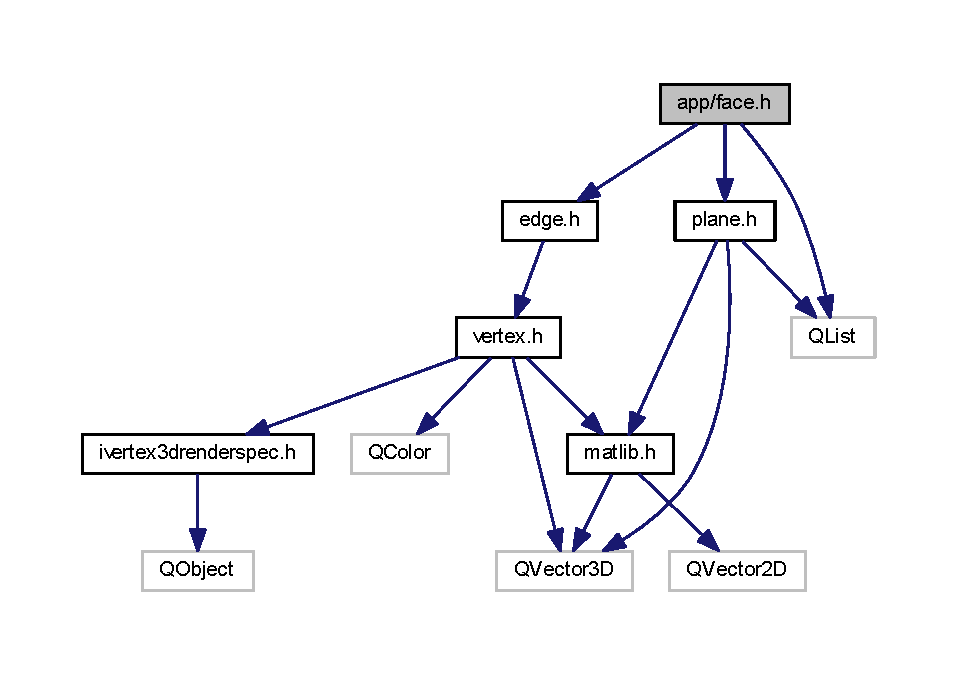
\includegraphics[width=350pt]{face_8h__incl}
\end{center}
\end{figure}
This graph shows which files directly or indirectly include this file\-:\nopagebreak
\begin{figure}[H]
\begin{center}
\leavevmode
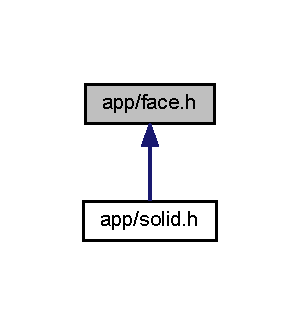
\includegraphics[width=144pt]{face_8h__dep__incl}
\end{center}
\end{figure}
\subsection*{Classes}
\begin{DoxyCompactItemize}
\item 
class \hyperlink{class_face3_d}{Face3\-D}
\begin{DoxyCompactList}\small\item\em Class representing a 3\-D face. \end{DoxyCompactList}\end{DoxyCompactItemize}


\subsection{Detailed Description}
Defines a 3\-D face. Solids are built up of these faces. Faces reference edges, which in turn reference vertices. 
\hypertarget{globals_8h}{\section{app/globals.h File Reference}
\label{globals_8h}\index{app/globals.\-h@{app/globals.\-h}}
}


Defines global variables and classes.  


{\ttfamily \#include $<$Q\-List$>$}\\*
{\ttfamily \#include \char`\"{}commandsenderinfo.\-h\char`\"{}}\\*
Include dependency graph for globals.\-h\-:\nopagebreak
\begin{figure}[H]
\begin{center}
\leavevmode
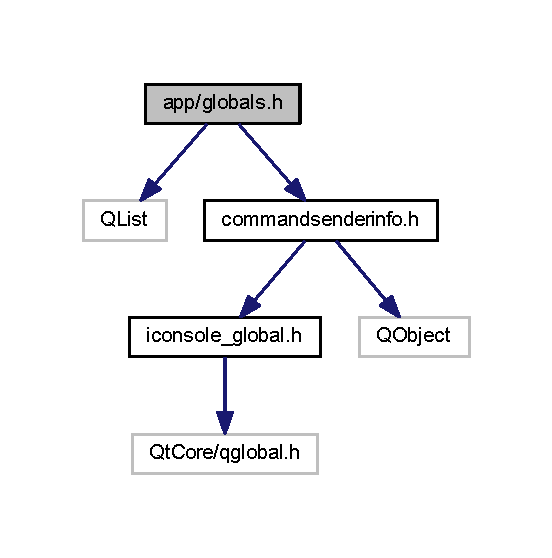
\includegraphics[width=265pt]{globals_8h__incl}
\end{center}
\end{figure}
\subsection*{Macros}
\begin{DoxyCompactItemize}
\item 
\#define \hyperlink{group___global_variables_gaf9c6d8de2e7b3d11f070bb500d62edce}{D\-E\-F\-I\-N\-E\-\_\-\-C\-O\-N\-V\-A\-R}(sz\-Name\-\_\-\-No\-Quote, sz\-Def\-Val, p\-Callback, sz\-Desc, i\-Flags, b\-Min, fl\-Min, b\-Max, fl\-Max)~\hyperlink{class_con_var}{Con\-Var} sz\-Name\-\_\-\-No\-Quote(\#sz\-Name\-\_\-\-No\-Quote, sz\-Def\-Val, \hyperlink{group___global_variables_ga4d39defaa5d22f29bde4c75d590bd0fe}{g\-\_\-p\-Command\-Manager}, \&\hyperlink{group___global_variables_ga8389c826239a1bc627ae3b7f97a79fe4}{g\-\_\-p\-Command\-List}, p\-Callback, sz\-Desc, i\-Flags, b\-Min, fl\-Min, b\-Max, fl\-Max);
\begin{DoxyCompactList}\small\item\em Macro for defining a \hyperlink{class_con_var}{Con\-Var} with the default command manager and list. \end{DoxyCompactList}\item 
\#define \hyperlink{group___global_variables_ga5c65583f94cc62a481b1846c0e6e3344}{D\-E\-F\-I\-N\-E\-\_\-\-C\-O\-N\-C\-O\-M\-M\-A\-N\-D}(sz\-Name\-\_\-\-No\-Quote, p\-Callback, sz\-Desc, i\-Flags)~\hyperlink{class_con_command}{Con\-Command} sz\-Name\-\_\-\-No\-Quote(\#sz\-Name\-\_\-\-No\-Quote, p\-Callback, \hyperlink{group___global_variables_ga4d39defaa5d22f29bde4c75d590bd0fe}{g\-\_\-p\-Command\-Manager}, \&\hyperlink{group___global_variables_ga8389c826239a1bc627ae3b7f97a79fe4}{g\-\_\-p\-Command\-List}, sz\-Desc, i\-Flags);
\begin{DoxyCompactList}\small\item\em Macro for defining a \hyperlink{class_con_command}{Con\-Command} with the default command manager and list. \end{DoxyCompactList}\end{DoxyCompactItemize}
\subsection*{Functions}
\begin{DoxyCompactItemize}
\item 
void \hyperlink{group___global_variables_ga9551f73a6927861d0b6f5d7901c90888}{Show\-Message\-Box} (Q\-String message)
\begin{DoxyCompactList}\small\item\em Creates a basic one-\/time modal message box with simple message and an \char`\"{}\-O\-K\char`\"{} button. \end{DoxyCompactList}\item 
void \hyperlink{group___global_variables_gadf8a13f3d23660f424828d7f559addd3}{Show\-Error\-Box} (Q\-String message)
\begin{DoxyCompactList}\small\item\em Creates a basic one-\/time modal error box with simple message and an \char`\"{}\-O\-K\char`\"{} button. \end{DoxyCompactList}\item 
void \hyperlink{group___global_variables_ga1788dc69b89b298a038015cbb83f8183}{Log\-Message} (const Q\-String \&message, bool newline=true)
\begin{DoxyCompactList}\small\item\em Logs a message to the log window. \end{DoxyCompactList}\item 
void \hyperlink{group___global_variables_gacb9fa8876388ad9319c61d9ae4d21510}{Log\-Tagged\-Message} (const Q\-String \&tag, const Q\-String \&message, bool newline=true)
\begin{DoxyCompactList}\small\item\em Logs a tagged message. \end{DoxyCompactList}\item 
void \hyperlink{group___global_variables_ga4b2863ab23932e06f2b5f292c66e7ef6}{Log\-Warning} (const Q\-String \&message, bool newline=true)
\begin{DoxyCompactList}\small\item\em Logs a warning to the log window. Log text is printed red and in bold. \end{DoxyCompactList}\item 
void \hyperlink{group___global_variables_ga49e471be032d9340fe6b4c251d1aef21}{Log\-Tagged\-Warning} (const Q\-String \&tag, const Q\-String \&message, bool newline=true)
\begin{DoxyCompactList}\small\item\em Logs a tagged warning to the log window. Log text is printed red and in bold. \end{DoxyCompactList}\item 
void \hyperlink{group___global_variables_gab9e5c16962c3cdcd7220de6dfa5a70b5}{Log\-Output} (\hyperlink{class_command_sender_info_a3a5e6a2ef1772f6557f351652c2e3b60}{Command\-Sender\-Info\-::\-Output\-Type} type, const Q\-String \&message, bool newline=true)
\begin{DoxyCompactList}\small\item\em Logs output of the specified type to the log window. \end{DoxyCompactList}\item 
void \hyperlink{group___global_variables_ga63348a368c397865f05d9a17c94752c6}{Log\-Tagged\-Output} (\hyperlink{class_command_sender_info_a3a5e6a2ef1772f6557f351652c2e3b60}{Command\-Sender\-Info\-::\-Output\-Type} type, const Q\-String \&tag, const Q\-String \&message, bool newline=true)
\begin{DoxyCompactList}\small\item\em Logs tagged output of the specified type to the log window. \end{DoxyCompactList}\end{DoxyCompactItemize}
\subsection*{Variables}
\begin{DoxyCompactItemize}
\item 
\hyperlink{class_command_line_parser}{Command\-Line\-Parser} $\ast$ \hyperlink{group___global_variables_ga270fc6d9322b018e011978d6376f43ba}{g\-\_\-p\-Cmd\-Line}
\begin{DoxyCompactList}\small\item\em Global command-\/line parser object. \end{DoxyCompactList}\item 
\hyperlink{class_console_window}{Console\-Window} $\ast$ \hyperlink{group___global_variables_gae2d76408535137add345d6e4258c5a07}{g\-\_\-p\-Log}
\begin{DoxyCompactList}\small\item\em Global console window object. \end{DoxyCompactList}\item 
Q\-List$<$ \hyperlink{class_main_win}{Main\-Win} $\ast$ $>$ $\ast$ \hyperlink{group___global_variables_gab5d481b5087f9956e533067ad8001d78}{g\-\_\-p\-Window\-Tracker}
\begin{DoxyCompactList}\small\item\em Global window tracker object. \end{DoxyCompactList}\item 
\hyperlink{class_listed_command_manager}{Listed\-Command\-Manager} $\ast$ \hyperlink{group___global_variables_ga4d39defaa5d22f29bde4c75d590bd0fe}{g\-\_\-p\-Command\-Manager}
\begin{DoxyCompactList}\small\item\em Global console command manager, created in main.\-cpp. \end{DoxyCompactList}\item 
\hypertarget{group___global_variables_ga347a4723fad5c3711958f787dfc93fa4}{\hyperlink{class_command_interpreter}{Command\-Interpreter} $\ast$ \hyperlink{group___global_variables_ga347a4723fad5c3711958f787dfc93fa4}{g\-\_\-p\-Command\-Interpreter}}\label{group___global_variables_ga347a4723fad5c3711958f787dfc93fa4}

\begin{DoxyCompactList}\small\item\em Global console command interpreter, created in main.\-cpp. \end{DoxyCompactList}\item 
\hyperlink{class_listed_console_command}{Listed\-Console\-Command} $\ast$ \hyperlink{group___global_variables_ga8389c826239a1bc627ae3b7f97a79fe4}{g\-\_\-p\-Command\-List}
\begin{DoxyCompactList}\small\item\em Global console command list pointer. \end{DoxyCompactList}\end{DoxyCompactItemize}


\subsection{Detailed Description}
Defines global variables and classes. This file defines certain classes and variables which should be visible from anywhere in the application. Examples include the command-\/line parser, the log window and the window tracker. Some classes or properties have convenience macros defined. 
\hypertarget{indexpool_8h}{\section{app/indexpool.h File Reference}
\label{indexpool_8h}\index{app/indexpool.\-h@{app/indexpool.\-h}}
}


Defines the \hyperlink{class_index_pool}{Index\-Pool} class which manages non-\/consecutive array indices.  


{\ttfamily \#include $<$Q\-Object$>$}\\*
{\ttfamily \#include $<$Q\-Map$>$}\\*
{\ttfamily \#include \char`\"{}vertex.\-h\char`\"{}}\\*
Include dependency graph for indexpool.\-h\-:\nopagebreak
\begin{figure}[H]
\begin{center}
\leavevmode
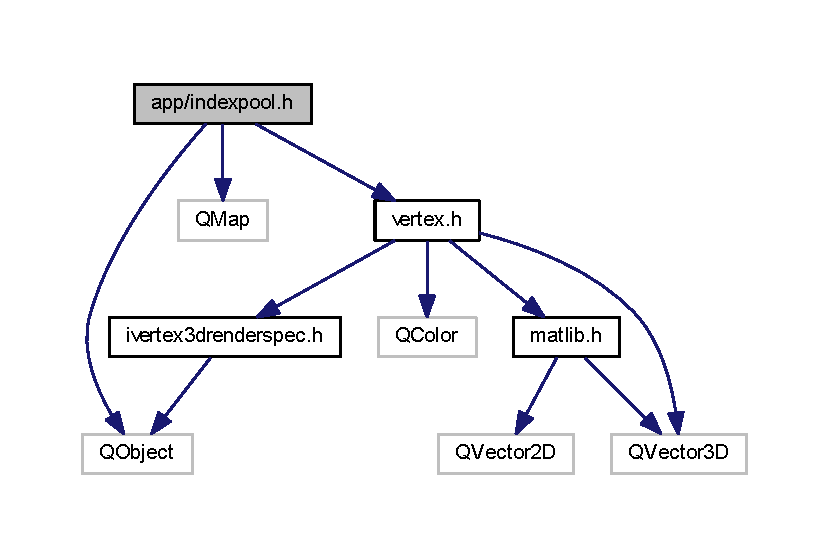
\includegraphics[width=350pt]{indexpool_8h__incl}
\end{center}
\end{figure}
This graph shows which files directly or indirectly include this file\-:\nopagebreak
\begin{figure}[H]
\begin{center}
\leavevmode
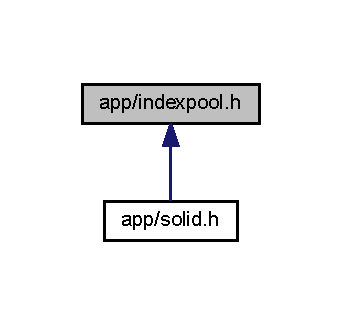
\includegraphics[width=164pt]{indexpool_8h__dep__incl}
\end{center}
\end{figure}
\subsection*{Classes}
\begin{DoxyCompactItemize}
\item 
class \hyperlink{class_index_pool}{Index\-Pool}
\begin{DoxyCompactList}\small\item\em The \hyperlink{class_index_pool}{Index\-Pool} class manages non-\/consecutive array indices. \end{DoxyCompactList}\end{DoxyCompactItemize}


\subsection{Detailed Description}
Defines the \hyperlink{class_index_pool}{Index\-Pool} class which manages non-\/consecutive array indices. 
\hypertarget{ivertex3drenderspec_8h}{\section{app/ivertex3drenderspec.h File Reference}
\label{ivertex3drenderspec_8h}\index{app/ivertex3drenderspec.\-h@{app/ivertex3drenderspec.\-h}}
}


Defines the interface between map vertices and the vertices used for rendering.  


{\ttfamily \#include $<$Q\-Object$>$}\\*
Include dependency graph for ivertex3drenderspec.\-h\-:\nopagebreak
\begin{figure}[H]
\begin{center}
\leavevmode
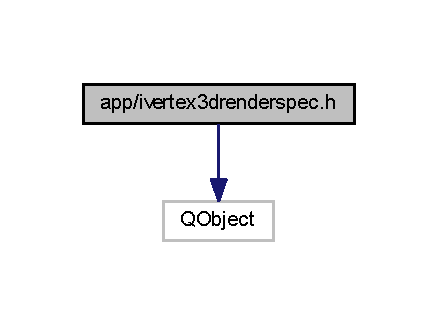
\includegraphics[width=210pt]{ivertex3drenderspec_8h__incl}
\end{center}
\end{figure}
This graph shows which files directly or indirectly include this file\-:\nopagebreak
\begin{figure}[H]
\begin{center}
\leavevmode
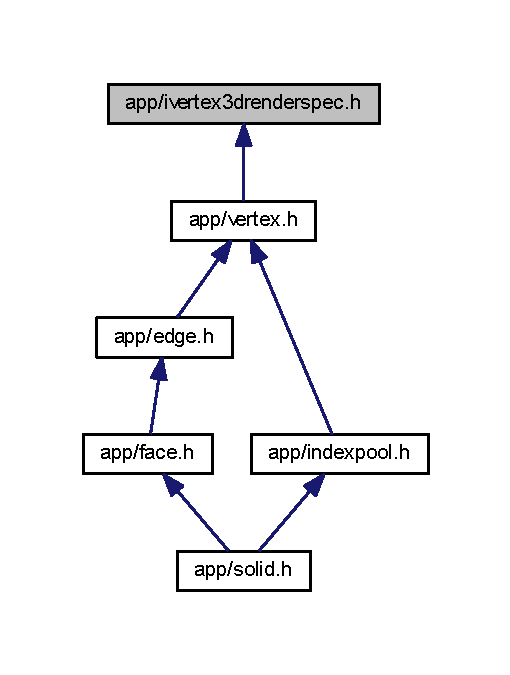
\includegraphics[width=245pt]{ivertex3drenderspec_8h__dep__incl}
\end{center}
\end{figure}
\subsection*{Classes}
\begin{DoxyCompactItemize}
\item 
class \hyperlink{class_i_vertex3_d_render_spec}{I\-Vertex3\-D\-Render\-Spec}
\begin{DoxyCompactList}\small\item\em Defines the properties required to be exposed by renderable vertices. \end{DoxyCompactList}\end{DoxyCompactItemize}
\subsection*{Macros}
\begin{DoxyCompactItemize}
\item 
\hypertarget{ivertex3drenderspec_8h_afd14dd1ec641943da1c3cd81a0037c0d}{\#define \hyperlink{ivertex3drenderspec_8h_afd14dd1ec641943da1c3cd81a0037c0d}{I\-Vertex3\-D\-Render\-Spec\-\_\-iid}~\char`\"{}Crowbar.\-Interfaces.\-I\-Vertex3\-D\-Render\-Spec\char`\"{}}\label{ivertex3drenderspec_8h_afd14dd1ec641943da1c3cd81a0037c0d}

\begin{DoxyCompactList}\small\item\em Unique I\-D for \hyperlink{class_i_vertex3_d_render_spec}{I\-Vertex3\-D\-Render\-Spec} interface. \end{DoxyCompactList}\end{DoxyCompactItemize}


\subsection{Detailed Description}
Defines the interface between map vertices and the vertices used for rendering. This file describes the requirements for a map vertex in terms of what information is required by the rendering engine. In order for a vertex to be rendered, it must implement these functions. 
\hypertarget{logwindow_8h}{\section{app/logwindow.h File Reference}
\label{logwindow_8h}\index{app/logwindow.\-h@{app/logwindow.\-h}}
}


Defines the logging window used when the application is in debug mode.  


{\ttfamily \#include $<$Q\-Widget$>$}\\*
Include dependency graph for logwindow.\-h\-:
\nopagebreak
\begin{figure}[H]
\begin{center}
\leavevmode
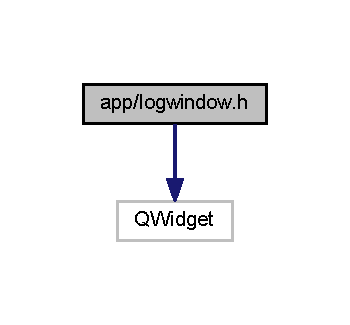
\includegraphics[width=168pt]{logwindow_8h__incl}
\end{center}
\end{figure}
\subsection*{Classes}
\begin{DoxyCompactItemize}
\item 
class \hyperlink{class_log_window}{Log\-Window}
\begin{DoxyCompactList}\small\item\em Logging window. \end{DoxyCompactList}\end{DoxyCompactItemize}
\subsection*{Macros}
\begin{DoxyCompactItemize}
\item 
\hypertarget{logwindow_8h_a25966c8a7f786f100610fc01ac4b434b}{\#define \hyperlink{logwindow_8h_a25966c8a7f786f100610fc01ac4b434b}{L\-O\-G\-\_\-\-Z\-O\-O\-M\-\_\-\-I\-N\-C\-R\-E\-M\-E\-N\-T}~2}\label{logwindow_8h_a25966c8a7f786f100610fc01ac4b434b}

\begin{DoxyCompactList}\small\item\em Increment with which to zoom in or out on \hyperlink{class_log_window_af2db9c420af21e1c07b416a6a3a7e5a2}{Log\-Window\-::zoom\-In()} or \hyperlink{class_log_window_ae534c7a6486b7223427dc2ad65316b09}{Log\-Window\-::zoom\-Out()}. \end{DoxyCompactList}\item 
\hypertarget{logwindow_8h_aa59f3c05c5e9a804278af23116d430b6}{\#define \hyperlink{logwindow_8h_aa59f3c05c5e9a804278af23116d430b6}{L\-O\-G\-\_\-\-W\-A\-R\-N\-I\-N\-G\-\_\-\-W\-E\-I\-G\-H\-T}~75}\label{logwindow_8h_aa59f3c05c5e9a804278af23116d430b6}

\begin{DoxyCompactList}\small\item\em Text weight of warning messages printed to the log window. \end{DoxyCompactList}\end{DoxyCompactItemize}


\subsection{Detailed Description}
Defines the logging window used when the application is in debug mode. 
\hypertarget{mainwin_8h}{\section{app/mainwin.h File Reference}
\label{mainwin_8h}\index{app/mainwin.\-h@{app/mainwin.\-h}}
}


Defines a main application window corresponding to one currently open map document.  


{\ttfamily \#include $<$Q\-Main\-Window$>$}\\*
{\ttfamily \#include $<$Q\-Application$>$}\\*
{\ttfamily \#include $<$Q\-Close\-Event$>$}\\*
Include dependency graph for mainwin.\-h\-:\nopagebreak
\begin{figure}[H]
\begin{center}
\leavevmode
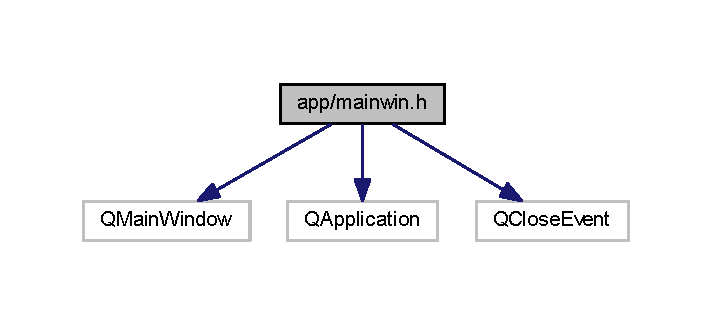
\includegraphics[width=341pt]{mainwin_8h__incl}
\end{center}
\end{figure}
\subsection*{Classes}
\begin{DoxyCompactItemize}
\item 
class \hyperlink{class_main_win}{Main\-Win}
\begin{DoxyCompactList}\small\item\em Application window class. \end{DoxyCompactList}\end{DoxyCompactItemize}


\subsection{Detailed Description}
Defines a main application window corresponding to one currently open map document. 
\hypertarget{mapdoc_8h}{\section{app/mapdoc.h File Reference}
\label{mapdoc_8h}\index{app/mapdoc.\-h@{app/mapdoc.\-h}}
}


The main map document class.  


{\ttfamily \#include $<$Q\-Object$>$}\\*
{\ttfamily \#include \char`\"{}octree/octree.\-h\char`\"{}}\\*
Include dependency graph for mapdoc.\-h\-:
\nopagebreak
\begin{figure}[H]
\begin{center}
\leavevmode
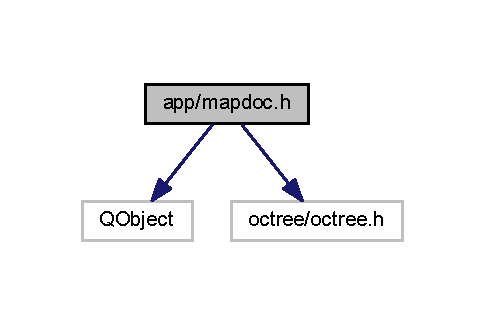
\includegraphics[width=233pt]{mapdoc_8h__incl}
\end{center}
\end{figure}
\subsection*{Classes}
\begin{DoxyCompactItemize}
\item 
class \hyperlink{class_map_doc}{Map\-Doc}
\begin{DoxyCompactList}\small\item\em The \hyperlink{class_map_doc}{Map\-Doc} class. \end{DoxyCompactList}\end{DoxyCompactItemize}
\subsection*{Macros}
\begin{DoxyCompactItemize}
\item 
\hypertarget{mapdoc_8h_af6699d6ffa298734e45b6a64604eb0ab}{\#define \hyperlink{mapdoc_8h_af6699d6ffa298734e45b6a64604eb0ab}{M\-A\-P\-D\-O\-C\-\_\-\-V\-E\-R\-S\-I\-O\-N}~10}\label{mapdoc_8h_af6699d6ffa298734e45b6a64604eb0ab}

\begin{DoxyCompactList}\small\item\em Current version of the mapdoc\-: \mbox{[}major\mbox{]}\mbox{[}minor\mbox{]}. \end{DoxyCompactList}\end{DoxyCompactItemize}


\subsection{Detailed Description}
The main map document class. The \hyperlink{class_map_doc}{Map\-Doc} class details any information that will be serialised when a map source file is saved. This includes geometry and entities but also settings such as camera positions, grid size, snapping, etc. Geometry and entities are kept inside an octree that represents the entire 3\-D space in the level.

\begin{DoxyNote}{Note}
Simon Perreault's octree's documentation can be found at \href{http://nomis80.org/code/doc/classOctree.html}{\tt http\-://nomis80.\-org/code/doc/class\-Octree.\-html} 
\end{DoxyNote}

\hypertarget{matlib_8h}{\section{app/matlib.h File Reference}
\label{matlib_8h}\index{app/matlib.\-h@{app/matlib.\-h}}
}


Contains convenient custom maths functions.  


{\ttfamily \#include $<$Q\-Vector3\-D$>$}\\*
{\ttfamily \#include $<$Q\-Vector2\-D$>$}\\*
Include dependency graph for matlib.\-h\-:
\nopagebreak
\begin{figure}[H]
\begin{center}
\leavevmode
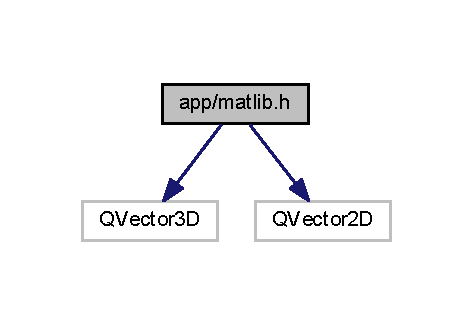
\includegraphics[width=227pt]{matlib_8h__incl}
\end{center}
\end{figure}
This graph shows which files directly or indirectly include this file\-:
\nopagebreak
\begin{figure}[H]
\begin{center}
\leavevmode
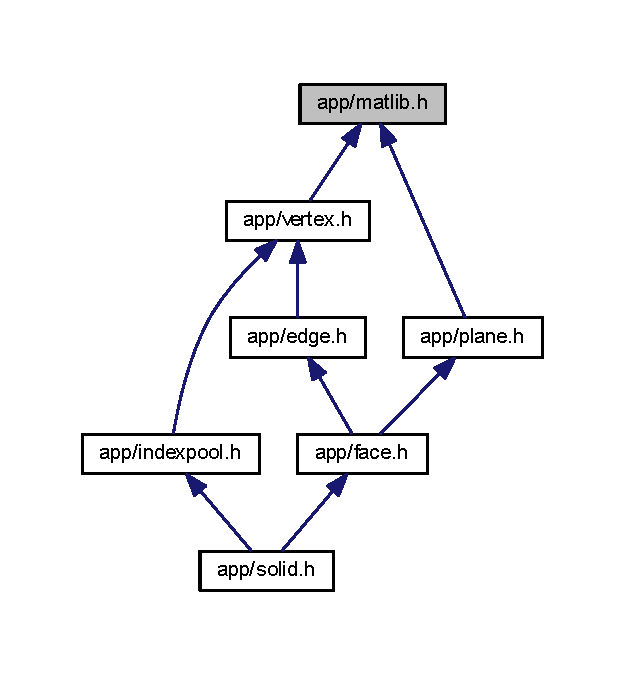
\includegraphics[width=300pt]{matlib_8h__dep__incl}
\end{center}
\end{figure}
\subsection*{Functions}
\begin{DoxyCompactItemize}
\item 
\hypertarget{matlib_8h_abbca97a4f576c9ea1a52b3ab4fe9a483}{static const Q\-Vector2\-D \hyperlink{matlib_8h_abbca97a4f576c9ea1a52b3ab4fe9a483}{V\-E\-C2\-\_\-\-O\-R\-I\-G\-I\-N} (0.\-0, 0.\-0)}\label{matlib_8h_abbca97a4f576c9ea1a52b3ab4fe9a483}

\begin{DoxyCompactList}\small\item\em Null 2\-D vector\-: (0.\-0, 0.\-0). \end{DoxyCompactList}\item 
\hypertarget{matlib_8h_ac2de4dab97258eff87e0a1253a2d1a29}{static const Q\-Vector3\-D \hyperlink{matlib_8h_ac2de4dab97258eff87e0a1253a2d1a29}{V\-E\-C3\-\_\-\-O\-R\-I\-G\-I\-N} (0.\-0, 0.\-0, 0.\-0)}\label{matlib_8h_ac2de4dab97258eff87e0a1253a2d1a29}

\begin{DoxyCompactList}\small\item\em Null 3\-D vector\-: (0.\-0, 0.\-0, 0.\-0). \end{DoxyCompactList}\end{DoxyCompactItemize}


\subsection{Detailed Description}
Contains convenient custom maths functions. 
\hypertarget{plane_8h}{\section{app/plane.h File Reference}
\label{plane_8h}\index{app/plane.\-h@{app/plane.\-h}}
}


Defines a plane class to hold the co-\/ordinates of a plane in 3\-D space.  


{\ttfamily \#include \char`\"{}matlib.\-h\char`\"{}}\\*
{\ttfamily \#include $<$Q\-Vector3\-D$>$}\\*
{\ttfamily \#include $<$Q\-List$>$}\\*
Include dependency graph for plane.\-h\-:
\nopagebreak
\begin{figure}[H]
\begin{center}
\leavevmode
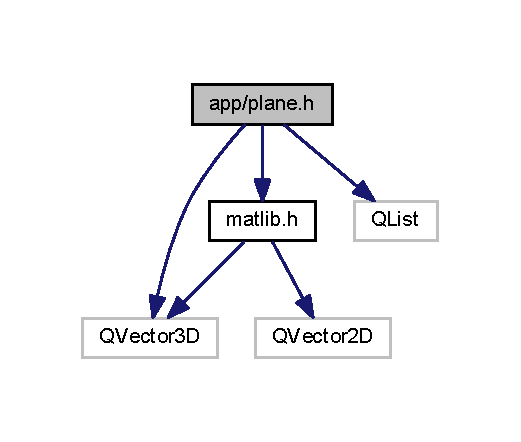
\includegraphics[width=250pt]{plane_8h__incl}
\end{center}
\end{figure}
This graph shows which files directly or indirectly include this file\-:
\nopagebreak
\begin{figure}[H]
\begin{center}
\leavevmode
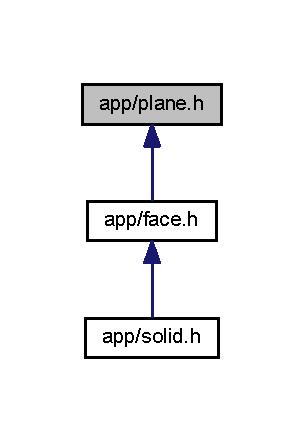
\includegraphics[width=146pt]{plane_8h__dep__incl}
\end{center}
\end{figure}
\subsection*{Classes}
\begin{DoxyCompactItemize}
\item 
class \hyperlink{class_plane}{Plane}
\begin{DoxyCompactList}\small\item\em Defines a plane in 3\-D space. \end{DoxyCompactList}\end{DoxyCompactItemize}


\subsection{Detailed Description}
Defines a plane class to hold the co-\/ordinates of a plane in 3\-D space. The plane class contains three points that define the plane and a normal that defines its front. Planes can be invalid, which means that two or more of their defining points are identical. 
\hypertarget{plugin_8h}{\section{app/plugin.h File Reference}
\label{plugin_8h}\index{app/plugin.\-h@{app/plugin.\-h}}
}


Defines interfaces for Crowbar extension plugins.  


{\ttfamily \#include $<$Qt\-Plugin$>$}\\*
Include dependency graph for plugin.\-h\-:
\nopagebreak
\begin{figure}[H]
\begin{center}
\leavevmode
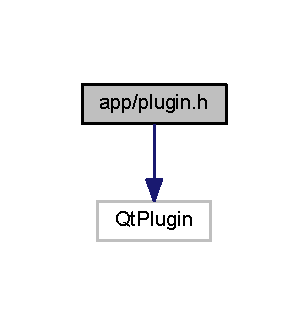
\includegraphics[width=148pt]{plugin_8h__incl}
\end{center}
\end{figure}
\subsection*{Classes}
\begin{DoxyCompactItemize}
\item 
class \hyperlink{class_i_plugin}{I\-Plugin}
\begin{DoxyCompactList}\small\item\em Required core interface for a Crowbar plugin. \end{DoxyCompactList}\end{DoxyCompactItemize}
\subsection*{Macros}
\begin{DoxyCompactItemize}
\item 
\hypertarget{plugin_8h_a9ab87d7ee5d55bff8a3c63aa85ed3862}{\#define \hyperlink{plugin_8h_a9ab87d7ee5d55bff8a3c63aa85ed3862}{I\-Plugin\-\_\-iid}~\char`\"{}Crowbar.\-Interfaces.\-I\-Plugin\char`\"{}}\label{plugin_8h_a9ab87d7ee5d55bff8a3c63aa85ed3862}

\begin{DoxyCompactList}\small\item\em Unique I\-D for \hyperlink{class_i_plugin}{I\-Plugin} interface. \end{DoxyCompactList}\end{DoxyCompactItemize}
\subsection*{Typedefs}
\begin{DoxyCompactItemize}
\item 
\hypertarget{plugin_8h_a725de6c68b62463ee6792bb48710febe}{typedef int \hyperlink{plugin_8h_a725de6c68b62463ee6792bb48710febe}{Plugin\-Version} \mbox{[}4\mbox{]}}\label{plugin_8h_a725de6c68b62463ee6792bb48710febe}

\begin{DoxyCompactList}\small\item\em Typedef for int\mbox{[}4\mbox{]} -\/ holds the plugin's major, minor, revision and build numbers. \end{DoxyCompactList}\end{DoxyCompactItemize}


\subsection{Detailed Description}
Defines interfaces for Crowbar extension plugins. At its core, every Crowbar plugin must implement the \hyperlink{class_i_plugin}{I\-Plugin} interface to be loaded by the application. 
\hypertarget{pluginmanager_8h}{\section{app/pluginmanager.h File Reference}
\label{pluginmanager_8h}\index{app/pluginmanager.\-h@{app/pluginmanager.\-h}}
}


Defines the manager for Crowbar plugins.  


{\ttfamily \#include $<$Q\-Object$>$}\\*
{\ttfamily \#include $<$Q\-String$>$}\\*
{\ttfamily \#include $<$Q\-Hash$>$}\\*
{\ttfamily \#include $<$Q\-Dir$>$}\\*
{\ttfamily \#include $<$Q\-List$>$}\\*
Include dependency graph for pluginmanager.\-h\-:
\nopagebreak
\begin{figure}[H]
\begin{center}
\leavevmode
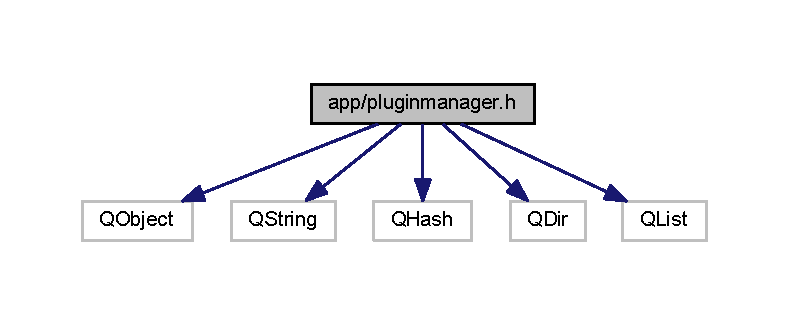
\includegraphics[width=350pt]{pluginmanager_8h__incl}
\end{center}
\end{figure}
\subsection*{Classes}
\begin{DoxyCompactItemize}
\item 
class \hyperlink{class_plugin_manager}{Plugin\-Manager}
\begin{DoxyCompactList}\small\item\em Manages loading of plugins. \end{DoxyCompactList}\end{DoxyCompactItemize}


\subsection{Detailed Description}
Defines the manager for Crowbar plugins. 
\hypertarget{property_8h}{\section{app/property.h File Reference}
\label{property_8h}\index{app/property.\-h@{app/property.\-h}}
}


Defines more specific typed properties that inherit from \hyperlink{class_base_property}{Base\-Property}.  


{\ttfamily \#include \char`\"{}baseproperty.\-h\char`\"{}}\\*
Include dependency graph for property.\-h\-:
\nopagebreak
\begin{figure}[H]
\begin{center}
\leavevmode
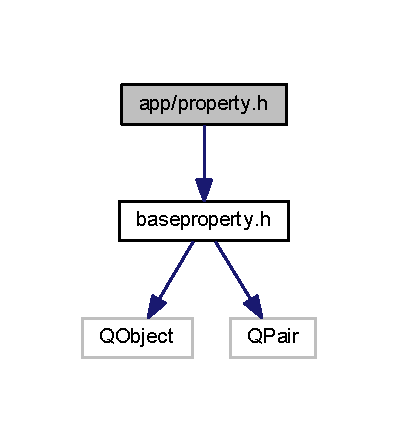
\includegraphics[width=191pt]{property_8h__incl}
\end{center}
\end{figure}
\subsection*{Classes}
\begin{DoxyCompactItemize}
\item 
class \hyperlink{class_i_string_property}{I\-String\-Property}
\begin{DoxyCompactList}\small\item\em M\-A\-C\-R\-O P\-R\-O\-P\-E\-R\-T\-Y I\-N\-T\-E\-R\-F\-A\-C\-E F\-O\-R Q\-String . \end{DoxyCompactList}\item 
class \hyperlink{class_w_string_property}{W\-String\-Property}
\begin{DoxyCompactList}\small\item\em M\-A\-C\-R\-O P\-R\-O\-P\-E\-R\-T\-Y I\-N\-T\-E\-R\-F\-A\-C\-E W\-R\-A\-P\-P\-E\-R F\-O\-R \hyperlink{class_i_string_property}{I\-String\-Property} . \end{DoxyCompactList}\item 
class \hyperlink{class_i_int_property}{I\-Int\-Property}
\begin{DoxyCompactList}\small\item\em M\-A\-C\-R\-O P\-R\-O\-P\-E\-R\-T\-Y I\-N\-T\-E\-R\-F\-A\-C\-E F\-O\-R int . \end{DoxyCompactList}\item 
class \hyperlink{class_w_int_property}{W\-Int\-Property}
\begin{DoxyCompactList}\small\item\em M\-A\-C\-R\-O P\-R\-O\-P\-E\-R\-T\-Y I\-N\-T\-E\-R\-F\-A\-C\-E W\-R\-A\-P\-P\-E\-R F\-O\-R \hyperlink{class_i_int_property}{I\-Int\-Property} . \end{DoxyCompactList}\item 
class \hyperlink{class_i_u_int_property}{I\-U\-Int\-Property}
\begin{DoxyCompactList}\small\item\em M\-A\-C\-R\-O P\-R\-O\-P\-E\-R\-T\-Y I\-N\-T\-E\-R\-F\-A\-C\-E F\-O\-R uint . \end{DoxyCompactList}\item 
class \hyperlink{class_w_u_int_property}{W\-U\-Int\-Property}
\begin{DoxyCompactList}\small\item\em M\-A\-C\-R\-O P\-R\-O\-P\-E\-R\-T\-Y I\-N\-T\-E\-R\-F\-A\-C\-E W\-R\-A\-P\-P\-E\-R F\-O\-R \hyperlink{class_i_u_int_property}{I\-U\-Int\-Property} . \end{DoxyCompactList}\item 
class \hyperlink{class_i_long_property}{I\-Long\-Property}
\begin{DoxyCompactList}\small\item\em M\-A\-C\-R\-O P\-R\-O\-P\-E\-R\-T\-Y I\-N\-T\-E\-R\-F\-A\-C\-E F\-O\-R long . \end{DoxyCompactList}\item 
class \hyperlink{class_w_long_property}{W\-Long\-Property}
\begin{DoxyCompactList}\small\item\em M\-A\-C\-R\-O P\-R\-O\-P\-E\-R\-T\-Y I\-N\-T\-E\-R\-F\-A\-C\-E W\-R\-A\-P\-P\-E\-R F\-O\-R \hyperlink{class_i_long_property}{I\-Long\-Property} . \end{DoxyCompactList}\item 
class \hyperlink{class_i_u_long_property}{I\-U\-Long\-Property}
\begin{DoxyCompactList}\small\item\em M\-A\-C\-R\-O P\-R\-O\-P\-E\-R\-T\-Y I\-N\-T\-E\-R\-F\-A\-C\-E F\-O\-R ulong . \end{DoxyCompactList}\item 
class \hyperlink{class_w_u_long_property}{W\-U\-Long\-Property}
\begin{DoxyCompactList}\small\item\em M\-A\-C\-R\-O P\-R\-O\-P\-E\-R\-T\-Y I\-N\-T\-E\-R\-F\-A\-C\-E W\-R\-A\-P\-P\-E\-R F\-O\-R \hyperlink{class_i_u_long_property}{I\-U\-Long\-Property} . \end{DoxyCompactList}\item 
class \hyperlink{class_i_float_property}{I\-Float\-Property}
\begin{DoxyCompactList}\small\item\em M\-A\-C\-R\-O P\-R\-O\-P\-E\-R\-T\-Y I\-N\-T\-E\-R\-F\-A\-C\-E F\-O\-R float . \end{DoxyCompactList}\item 
class \hyperlink{class_w_float_property}{W\-Float\-Property}
\begin{DoxyCompactList}\small\item\em M\-A\-C\-R\-O P\-R\-O\-P\-E\-R\-T\-Y I\-N\-T\-E\-R\-F\-A\-C\-E W\-R\-A\-P\-P\-E\-R F\-O\-R \hyperlink{class_i_float_property}{I\-Float\-Property} . \end{DoxyCompactList}\item 
class \hyperlink{class_i_double_property}{I\-Double\-Property}
\begin{DoxyCompactList}\small\item\em M\-A\-C\-R\-O P\-R\-O\-P\-E\-R\-T\-Y I\-N\-T\-E\-R\-F\-A\-C\-E F\-O\-R double . \end{DoxyCompactList}\item 
class \hyperlink{class_w_double_property}{W\-Double\-Property}
\begin{DoxyCompactList}\small\item\em M\-A\-C\-R\-O P\-R\-O\-P\-E\-R\-T\-Y I\-N\-T\-E\-R\-F\-A\-C\-E W\-R\-A\-P\-P\-E\-R F\-O\-R \hyperlink{class_i_double_property}{I\-Double\-Property} . \end{DoxyCompactList}\item 
class \hyperlink{class_i_long_long_property}{I\-Long\-Long\-Property}
\begin{DoxyCompactList}\small\item\em M\-A\-C\-R\-O P\-R\-O\-P\-E\-R\-T\-Y I\-N\-T\-E\-R\-F\-A\-C\-E F\-O\-R qlonglong . \end{DoxyCompactList}\item 
class \hyperlink{class_w_long_long_property}{W\-Long\-Long\-Property}
\begin{DoxyCompactList}\small\item\em M\-A\-C\-R\-O P\-R\-O\-P\-E\-R\-T\-Y I\-N\-T\-E\-R\-F\-A\-C\-E W\-R\-A\-P\-P\-E\-R F\-O\-R \hyperlink{class_i_long_long_property}{I\-Long\-Long\-Property} . \end{DoxyCompactList}\item 
class \hyperlink{class_i_u_long_long_property}{I\-U\-Long\-Long\-Property}
\begin{DoxyCompactList}\small\item\em M\-A\-C\-R\-O P\-R\-O\-P\-E\-R\-T\-Y I\-N\-T\-E\-R\-F\-A\-C\-E F\-O\-R qulonglong . \end{DoxyCompactList}\item 
class \hyperlink{class_w_u_long_long_property}{W\-U\-Long\-Long\-Property}
\begin{DoxyCompactList}\small\item\em M\-A\-C\-R\-O P\-R\-O\-P\-E\-R\-T\-Y I\-N\-T\-E\-R\-F\-A\-C\-E W\-R\-A\-P\-P\-E\-R F\-O\-R \hyperlink{class_i_u_long_long_property}{I\-U\-Long\-Long\-Property} . \end{DoxyCompactList}\item 
class \hyperlink{class_string_property}{String\-Property}
\begin{DoxyCompactList}\small\item\em The \hyperlink{class_string_property}{String\-Property} class Class that handles string properties. \end{DoxyCompactList}\item 
class \hyperlink{class_int_property}{Int\-Property}
\begin{DoxyCompactList}\small\item\em M\-A\-C\-R\-O P\-R\-O\-P\-E\-R\-T\-Y F\-O\-R int . \end{DoxyCompactList}\item 
class \hyperlink{class_u_int_property}{U\-Int\-Property}
\begin{DoxyCompactList}\small\item\em M\-A\-C\-R\-O P\-R\-O\-P\-E\-R\-T\-Y F\-O\-R uint . \end{DoxyCompactList}\item 
class \hyperlink{class_long_property}{Long\-Property}
\begin{DoxyCompactList}\small\item\em M\-A\-C\-R\-O P\-R\-O\-P\-E\-R\-T\-Y F\-O\-R long . \end{DoxyCompactList}\item 
class \hyperlink{class_u_long_property}{U\-Long\-Property}
\begin{DoxyCompactList}\small\item\em M\-A\-C\-R\-O P\-R\-O\-P\-E\-R\-T\-Y F\-O\-R ulong . \end{DoxyCompactList}\item 
class \hyperlink{class_float_property}{Float\-Property}
\begin{DoxyCompactList}\small\item\em M\-A\-C\-R\-O P\-R\-O\-P\-E\-R\-T\-Y F\-O\-R float . \end{DoxyCompactList}\item 
class \hyperlink{class_double_property}{Double\-Property}
\begin{DoxyCompactList}\small\item\em M\-A\-C\-R\-O P\-R\-O\-P\-E\-R\-T\-Y F\-O\-R double . \end{DoxyCompactList}\item 
class \hyperlink{class_long_long_property}{Long\-Long\-Property}
\begin{DoxyCompactList}\small\item\em M\-A\-C\-R\-O P\-R\-O\-P\-E\-R\-T\-Y F\-O\-R qlonglong . \end{DoxyCompactList}\item 
class \hyperlink{class_u_long_long_property}{U\-Long\-Long\-Property}
\begin{DoxyCompactList}\small\item\em M\-A\-C\-R\-O P\-R\-O\-P\-E\-R\-T\-Y F\-O\-R qulonglong . \end{DoxyCompactList}\end{DoxyCompactItemize}
\subsection*{Macros}
\begin{DoxyCompactItemize}
\item 
\#define \hyperlink{group___property_classes_gaac09fb32e07282e79330aeb7cfc9e5eb}{D\-E\-C\-L\-A\-R\-E\-\_\-\-P\-R\-O\-P\-E\-R\-T\-Y\-\_\-\-I\-N\-T\-E\-R\-F\-A\-C\-E}(\-\_\-classname, \-\_\-wrapper, \-\_\-type)
\begin{DoxyCompactList}\small\item\em Declares a property interface with an interface classname, wrapper classname and data type (such as int). \end{DoxyCompactList}\item 
\#define \hyperlink{group___property_classes_ga9b75216621cf38585610f12ce907d01c}{D\-E\-C\-L\-A\-R\-E\-\_\-\-N\-U\-M\-P\-R\-O\-P}(\-\_\-classname, \-\_\-interface, \-\_\-wrapper, \-\_\-type, \-\_\-proptype, \-\_\-vnull)
\begin{DoxyCompactList}\small\item\em Declares a number-\/type property which Q\-String has the capability to convert to and from, in macro form for convenience. \end{DoxyCompactList}\item 
\#define \hyperlink{group___property_classes_gae16b8183fbdf59c5bf8809835a2617e5}{I\-M\-P\-L\-E\-M\-E\-N\-T\-\_\-\-N\-U\-M\-P\-R\-O\-P}(\-\_\-classname, \-\_\-wrapper, \-\_\-type, \-\_\-cvtfunc, \-\_\-variantfunc)
\begin{DoxyCompactList}\small\item\em Implements the functions for a property declared previously with D\-E\-C\-L\-A\-R\-E\-\_\-\-N\-U\-M\-P\-R\-O\-P. \end{DoxyCompactList}\end{DoxyCompactItemize}


\subsection{Detailed Description}
Defines more specific typed properties that inherit from \hyperlink{class_base_property}{Base\-Property}. The property classes hold a key and a value -\/ these are underlyingly represented as strings and \hyperlink{class_base_property}{Base\-Property} subclasses deal with binding these solidly to interfaces for a specific type. A property's key should endeavour to be unique (it is not defined which property will be selected if two properties have the same key). \par
 \par
 A technical note\-: due to the Qt limitation that only one inheritance of the Q\-Object class is allowed for any derived class (slots requiring an interface inherit from Q\-Object), slots on property classes are exposed through a wrapper returned by calling slots\-For() on the property. Connecting a signal to a slot on this wrapper will call the relevant non-\/slot function on the property class. 
\hypertarget{solid_8h}{\section{app/solid.h File Reference}
\label{solid_8h}\index{app/solid.\-h@{app/solid.\-h}}
}


Defines a solid class.  


{\ttfamily \#include $<$Q\-Vector$>$}\\*
{\ttfamily \#include \char`\"{}face.\-h\char`\"{}}\\*
{\ttfamily \#include \char`\"{}indexpool.\-h\char`\"{}}\\*
Include dependency graph for solid.\-h\-:
\nopagebreak
\begin{figure}[H]
\begin{center}
\leavevmode
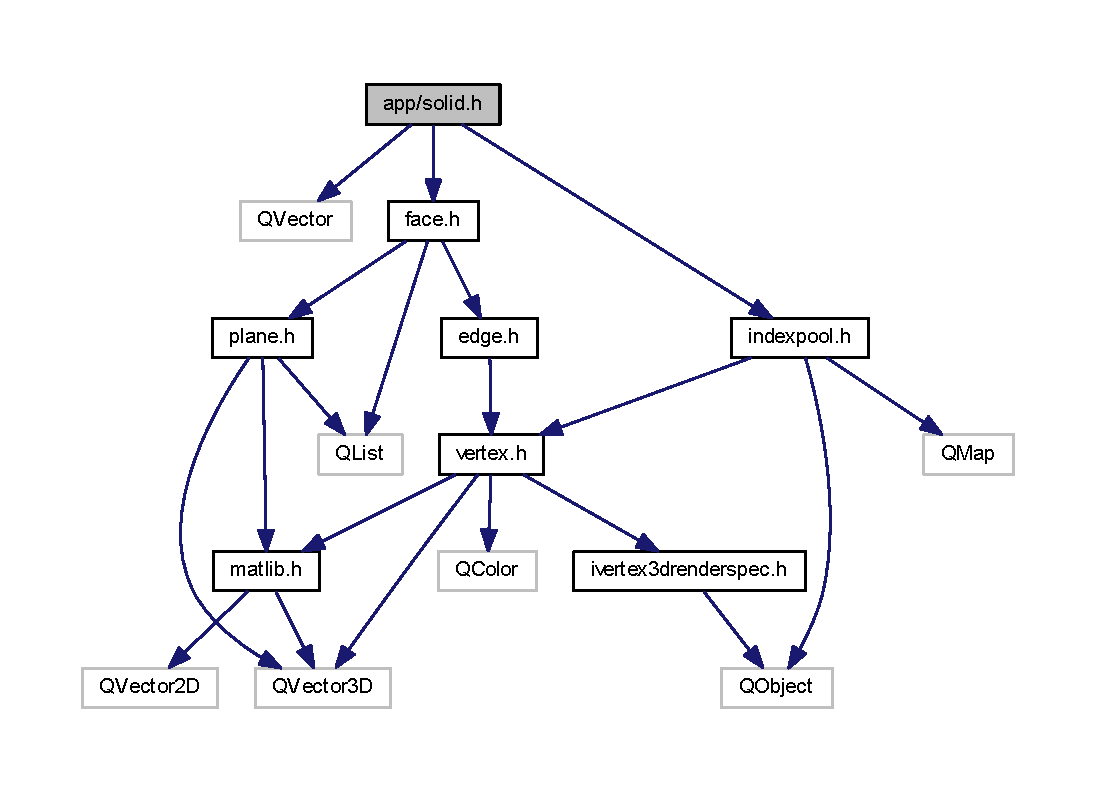
\includegraphics[width=350pt]{solid_8h__incl}
\end{center}
\end{figure}
\subsection*{Classes}
\begin{DoxyCompactItemize}
\item 
struct \hyperlink{struct_geom_info}{Geom\-Info}
\begin{DoxyCompactList}\small\item\em Struct to hold and pass information about geometry objects. \end{DoxyCompactList}\item 
class \hyperlink{class_solid3_d}{Solid3\-D}
\begin{DoxyCompactList}\small\item\em Class representing a 3\-D solid. \end{DoxyCompactList}\end{DoxyCompactItemize}


\subsection{Detailed Description}
Defines a solid class. Solids are the programmatical implementation of brushes and are made up of sets of vertices, edges and faces. Each edge references the vertices it links, and each face is built from multiple edges. As opposed to Hammer's implementation, solids are mesh-\/based (ie. they are defined by vertex positions and links rather than planes and intersections) to allow for easier manipulation, and are exported as plane-\/based objects when serialised as a V\-M\-F.\par
 It is recommended to work {\bfseries bottom-\/up} (ie. add any required vertices before edges, and edges before faces) rather than {\bfseries top-\/down} (creating all of a face's edges and vertices as the face itself is created) as the former method is less prone to errors. 
\hypertarget{vertex_8h}{\section{app/vertex.h File Reference}
\label{vertex_8h}\index{app/vertex.\-h@{app/vertex.\-h}}
}


T\-O\-D\-O.  


{\ttfamily \#include \char`\"{}matlib.\-h\char`\"{}}\\*
{\ttfamily \#include $<$Q\-Vector3\-D$>$}\\*
{\ttfamily \#include $<$Q\-Color$>$}\\*
{\ttfamily \#include \char`\"{}ivertex3drenderspec.\-h\char`\"{}}\\*
Include dependency graph for vertex.\-h\-:
\nopagebreak
\begin{figure}[H]
\begin{center}
\leavevmode
\includegraphics[width=350pt]{vertex_8h__incl}
\end{center}
\end{figure}
This graph shows which files directly or indirectly include this file\-:
\nopagebreak
\begin{figure}[H]
\begin{center}
\leavevmode
\includegraphics[width=245pt]{vertex_8h__dep__incl}
\end{center}
\end{figure}
\subsection*{Classes}
\begin{DoxyCompactItemize}
\item 
class \hyperlink{class_geom_meta_handle}{Geom\-Meta\-Handle}
\begin{DoxyCompactList}\small\item\em Metaclass which all geometry components subclass from. Contains useful metadata relevant to geometry components. \end{DoxyCompactList}\item 
class \hyperlink{class_vertex3_d}{Vertex3\-D}
\begin{DoxyCompactList}\small\item\em Defines a vertex in 3\-D space. \end{DoxyCompactList}\end{DoxyCompactItemize}
\subsection*{Macros}
\begin{DoxyCompactItemize}
\item 
\hypertarget{vertex_8h_a58600f71cdacd3fb41515de8749fe861}{\#define \hyperlink{vertex_8h_a58600f71cdacd3fb41515de8749fe861}{N\-U\-L\-L\-H\-N\-D}~0}\label{vertex_8h_a58600f71cdacd3fb41515de8749fe861}

\begin{DoxyCompactList}\small\item\em Value of a null G\-E\-O\-M\-H\-A\-N\-D\-L\-E. \end{DoxyCompactList}\end{DoxyCompactItemize}
\subsection*{Typedefs}
\begin{DoxyCompactItemize}
\item 
\hypertarget{vertex_8h_a72202e57358ed73cd212e9a2eaf39aeb}{typedef unsigned long \hyperlink{vertex_8h_a72202e57358ed73cd212e9a2eaf39aeb}{G\-E\-O\-M\-H\-A\-N\-D\-L\-E}}\label{vertex_8h_a72202e57358ed73cd212e9a2eaf39aeb}

\begin{DoxyCompactList}\small\item\em Handle for a geometry component. \end{DoxyCompactList}\item 
\hypertarget{vertex_8h_a2e2e1374aac5842116c8683f3b06e99f}{typedef unsigned long \hyperlink{vertex_8h_a2e2e1374aac5842116c8683f3b06e99f}{V\-B\-O\-\_\-\-O\-F\-F\-S\-E\-T}}\label{vertex_8h_a2e2e1374aac5842116c8683f3b06e99f}

\begin{DoxyCompactList}\small\item\em Value for specifying an offset in the graphics V\-B\-O. \end{DoxyCompactList}\end{DoxyCompactItemize}


\subsection{Detailed Description}
T\-O\-D\-O. 
\hypertarget{icommandbox_8h}{\section{I\-Console/interfaces/icommandbox.h File Reference}
\label{icommandbox_8h}\index{I\-Console/interfaces/icommandbox.\-h@{I\-Console/interfaces/icommandbox.\-h}}
}


Interface for command box (where commands are typed).  


{\ttfamily \#include \char`\"{}iconsole\-\_\-global.\-h\char`\"{}}\\*
Include dependency graph for icommandbox.\-h\-:
\nopagebreak
\begin{figure}[H]
\begin{center}
\leavevmode
\includegraphics[width=178pt]{icommandbox_8h__incl}
\end{center}
\end{figure}
\subsection*{Classes}
\begin{DoxyCompactItemize}
\item 
class \hyperlink{class_i_command_box}{I\-Command\-Box}
\end{DoxyCompactItemize}
\subsection*{Macros}
\begin{DoxyCompactItemize}
\item 
\hypertarget{icommandbox_8h_a1bcdc417fec2fc4b28edabfb2bb06c25}{\#define \hyperlink{icommandbox_8h_a1bcdc417fec2fc4b28edabfb2bb06c25}{I\-Command\-Box\-\_\-iid}~\char`\"{}Crowbar.\-Interfaces.\-I\-Console.\-I\-Command\-Box\char`\"{}}\label{icommandbox_8h_a1bcdc417fec2fc4b28edabfb2bb06c25}

\begin{DoxyCompactList}\small\item\em Unique I\-D for \hyperlink{class_i_command_box}{I\-Command\-Box} interface. \end{DoxyCompactList}\end{DoxyCompactItemize}


\subsection{Detailed Description}
Interface for command box (where commands are typed). 
\hypertarget{icommandmanager_8h}{\section{I\-Console/interfaces/icommandmanager.h File Reference}
\label{icommandmanager_8h}\index{I\-Console/interfaces/icommandmanager.\-h@{I\-Console/interfaces/icommandmanager.\-h}}
}


Defines the command manager interface.  


{\ttfamily \#include \char`\"{}iconsole\-\_\-global.\-h\char`\"{}}\\*
Include dependency graph for icommandmanager.\-h\-:
\nopagebreak
\begin{figure}[H]
\begin{center}
\leavevmode
\includegraphics[width=190pt]{icommandmanager_8h__incl}
\end{center}
\end{figure}
\subsection*{Classes}
\begin{DoxyCompactItemize}
\item 
class \hyperlink{class_i_command_manager}{I\-Command\-Manager}
\end{DoxyCompactItemize}
\subsection*{Macros}
\begin{DoxyCompactItemize}
\item 
\hypertarget{icommandmanager_8h_af0732cfb4c99c335dd3f6913dd3ce213}{\#define \hyperlink{icommandmanager_8h_af0732cfb4c99c335dd3f6913dd3ce213}{I\-Command\-Manager\-\_\-iid}~\char`\"{}Crowbar.\-Interfaces.\-I\-Console.\-I\-Command\-Manager\char`\"{}}\label{icommandmanager_8h_af0732cfb4c99c335dd3f6913dd3ce213}

\begin{DoxyCompactList}\small\item\em Unique I\-D for \hyperlink{class_i_command_manager}{I\-Command\-Manager} interface. \end{DoxyCompactList}\end{DoxyCompactItemize}


\subsection{Detailed Description}
Defines the command manager interface. 
\hypertarget{iconsolewindow_8h}{\section{I\-Console/interfaces/iconsolewindow.h File Reference}
\label{iconsolewindow_8h}\index{I\-Console/interfaces/iconsolewindow.\-h@{I\-Console/interfaces/iconsolewindow.\-h}}
}


Interface for console window.  


{\ttfamily \#include \char`\"{}iconsole\-\_\-global.\-h\char`\"{}}\\*
Include dependency graph for iconsolewindow.\-h\-:
\nopagebreak
\begin{figure}[H]
\begin{center}
\leavevmode
\includegraphics[width=178pt]{iconsolewindow_8h__incl}
\end{center}
\end{figure}
This graph shows which files directly or indirectly include this file\-:
\nopagebreak
\begin{figure}[H]
\begin{center}
\leavevmode
\includegraphics[width=210pt]{iconsolewindow_8h__dep__incl}
\end{center}
\end{figure}
\subsection*{Classes}
\begin{DoxyCompactItemize}
\item 
class \hyperlink{class_i_console_window}{I\-Console\-Window}
\end{DoxyCompactItemize}
\subsection*{Macros}
\begin{DoxyCompactItemize}
\item 
\hypertarget{iconsolewindow_8h_af6f0bb613cbcad5dc57d0deb74a770e8}{\#define \hyperlink{iconsolewindow_8h_af6f0bb613cbcad5dc57d0deb74a770e8}{I\-Console\-Window\-\_\-iid}~\char`\"{}Crowbar.\-Interfaces.\-I\-Console.\-I\-Console\-Window\char`\"{}}\label{iconsolewindow_8h_af6f0bb613cbcad5dc57d0deb74a770e8}

\begin{DoxyCompactList}\small\item\em Unique I\-D for \hyperlink{class_i_console_window}{I\-Console\-Window} interface. \end{DoxyCompactList}\end{DoxyCompactItemize}


\subsection{Detailed Description}
Interface for console window. 
%--- End generated contents ---

% Index
\newpage
\phantomsection
\addcontentsline{toc}{part}{Index}
\printindex

\end{document}
